%!TEX  root=./LIVRO.tex

\chapter{9. \emph{Karawara}}\label{karawara}

\begin{figure}[H]
\centering
  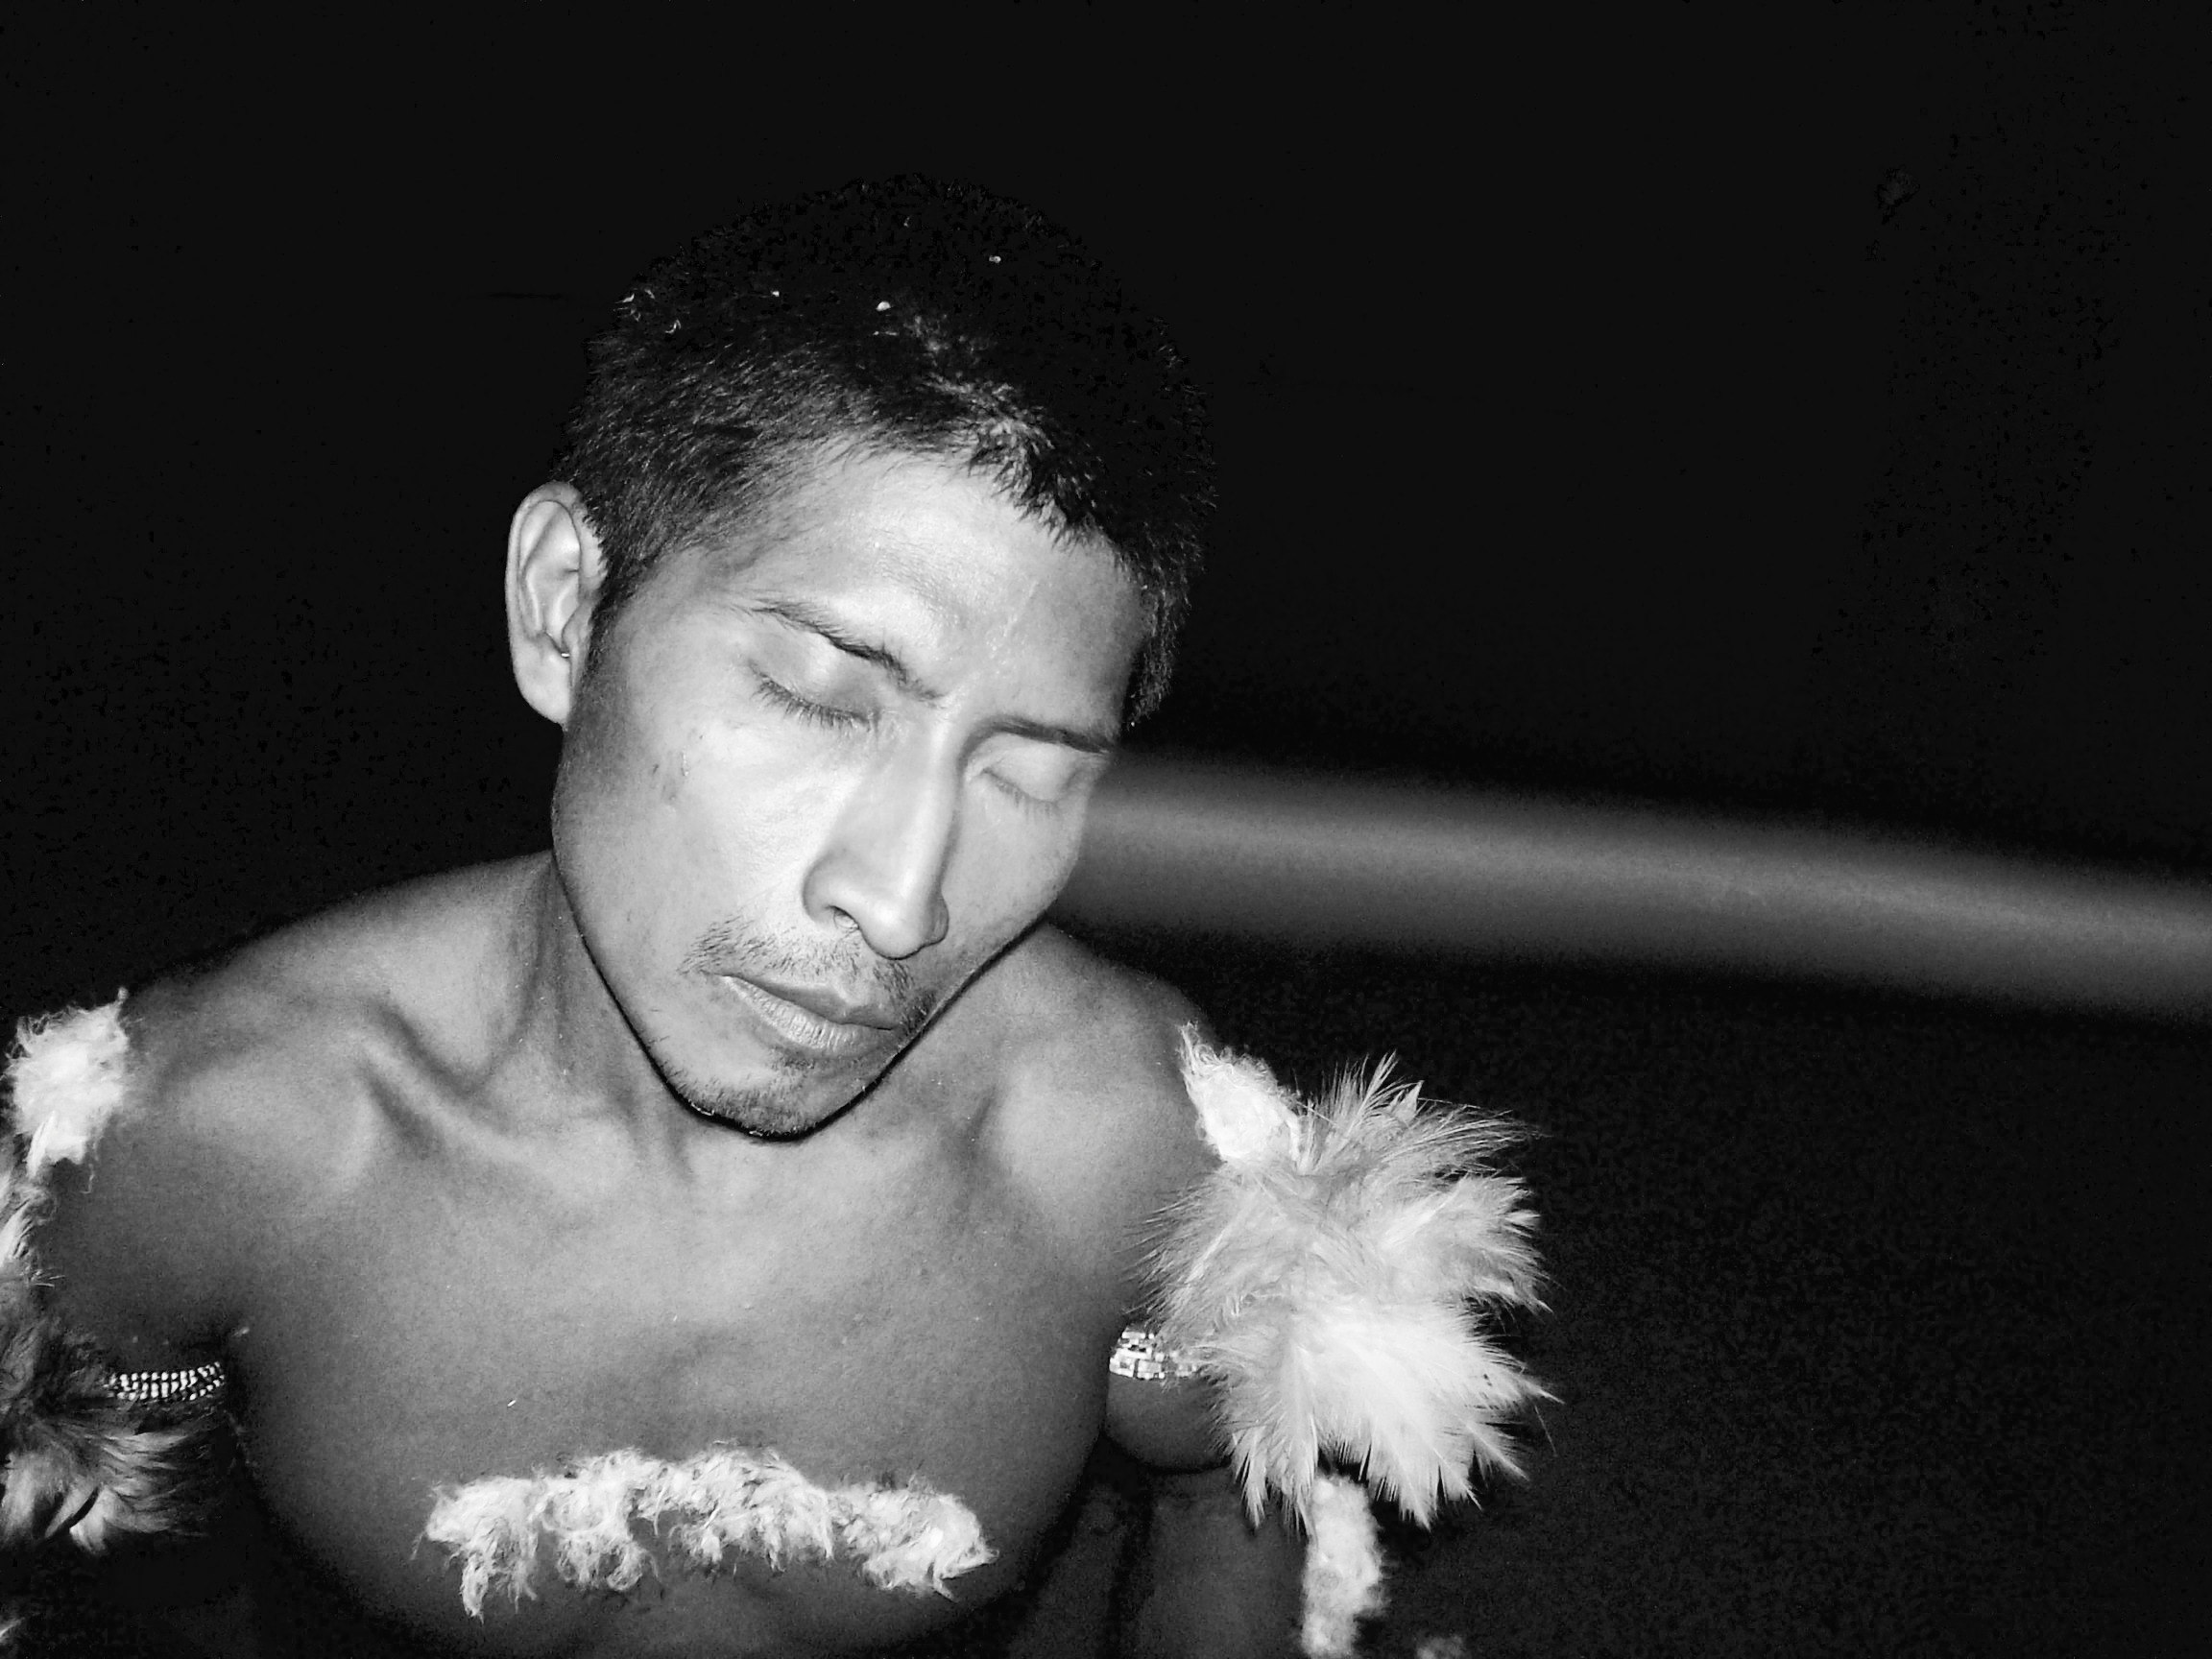
\includegraphics[width=\textwidth]{./imgs/100_1752}
\caption{Um karawara trazido pelo irmão de Wiraho e Hemokoma’a durante a cantoria na takaja. Juriti, 2008.}
\end{figure}

\begin{quote}
\emph{Se eu morrer, minha pele fica na Terra, as pegadas do meu pé
ficam na Terra}.

\noindent
\emph{Minha pele torna"-se ajỹ. Meu coração, minha alma e minha carne vão
para o céu.}

\noindent
\emph{Ficam vivas. Ficam no céu, tornam"-se karawara. Ficam cantando,
dançando, transformados em karawara.}

\noindent
\emph{As penas brancas e as vermelhas (que adornam os karawara) ficam no
céu}.

\begin{flushright}
\emph{(Irakatakoa, aldeia Awá, 2006)}\footnotemark
\end{flushright}

\footnotetext{\emph{Amanõ xi, ikwẽ ha pirera
  wype, ha pyporera wype.}

  \emph{Ha pirera iko ajỹ neme. Ha ja'ajna, ha ritekera, ha'okera oho
  iwape.}

  \emph{Ikwẽ. Iku iwape, iku karawa neme.}

  \emph{Jã ika, panỹ ika, oho karawa neme.}

  \emph{Hawiju, japakwa iku iwape}.

  Coletado e traduzido por Marina Magalhães, 2006.}
\end{quote}

\noindent Os \emph{karawara}, como mencionado em outras partes do livro, são uma
complexa classe de seres que povoam os patamares celestes e atuam na
Terra de diversas maneiras. São caçadores infalíveis, ao mesmo tempo que
espíritos auxiliares no xamanismo; são o destino de todo ser humano
(\emph{awatea}) após a morte, porém têm uma existência independente,
desvinculada da morte terrena. Os \emph{karawara} são ``gente''
(\emph{awa}), dizem os meus amigos, humanos de verdade (\emph{awatea}),
porém uma gente que vive no céu; são relacionados a pequenos mamíferos,
sapos, insetos de todo tipo, plantas, fenômenos naturais, objetos,
plantas cultivadas (como a macaxeira), mas sobretudo a aves. Pombas,
gaviões, rolinhas, beija"-flores, pica"-paus, socós, juritis, dentre
outros, são gente no céu, e cada \emph{karawara} ganha na Terra um
``correspondente'', que são como suas extensões terrenas. Nos patamares
celestes (\emph{iwa}) se conformam como diferentes tipos de gente como
uma gente pica"-pau, gente juriti, gente tucano, papagaio, siricora,
sabiá, várias borboletas, marimbondo, gente"-taquara, dentre outras
plantas e bichos, também referidos como \emph{jara}. Por serem exímios
caçadores e embora vivam no céu (\emph{iwa}), mantêm um trânsito
constante com a Terra, para onde descem a fim de buscar, basicamente,
caça, água, mel e, por vezes, fogo, produtos essenciais ao desenrolar da
vida celeste. Têm uma imagem humana celestial definida: bem adornados
com cocares e braceletes, habitantes de um lugar limpo e agradável,
caçadores infalíveis, cantores magníficos e falantes de uma outra
língua, uma fala celeste (\emph{iwa ma'iha} ``fala do céu'') cuja
prosódia é o canto (\emph{jãnaha}). Uma gente celeste cujas carcaças
animais (as ``pegadas'', \emph{ipopokera}) seriam suas formas terrenas.
Em poucas palavras, seriam \emph{eles}, ao mesmo tempo, caçadores e
xamãs magníficos.

Ao descerem à Terra (para caçar, extrair mel ou buscar água), os humanos
não os encontram, pois, além de serem rápidos em suas caçadas (como
veremos adiante), as realizam em locais e matas distantes, onde os Guajá
não alcançam. Se perguntarmos a uma pessoa das aldeias Jurití, Awá ou
Tiracambu sobre ``o que é'' um \emph{karawara}, provavelmente teremos
respostas como: \emph{awa} \emph{parãhy} (``são humanos belos''); ou
\emph{awaete} (``são gente de verdade''); ou \emph{awa} \emph{katy} (``são
pessoas boas''); ou ainda, \emph{karawara} \emph{wate} (``os
\emph{karawara} estão lá em cima''). E mesmo em português, quando queriam
me fazer entender, falavam ``\emph{mesminho eu, mesminho eu!}'', algo como
``são exatamente como nós somos!'' Além disso, os \emph{karawara} são
sempre referidos como ``\emph{parentes}'' (quando falam em português), uma
ideia que englobaria todas as acima. Ao mesmo tempo, como veremos, os
\emph{karawara}, mais do que ``entidades celestes'', são princípios de
ação (xamânica e cinegética) que desafiam a lógica de nosso entendimento
metafísico, não podendo ser enquadrados apenas como seres (ou
substâncias) ou apenas como fazeres (ou procedimentos). No decorrer do
livro já mencionei os \emph{karawara} algumas vezes, porém neste
capítulo gostaria de apresentá"-los mais detalhadamente e buscar algumas
conexões com o que já escrevi até aqui, principalmente no que se refere
às ideias de \emph{jara}, \emph{nima} e \emph{riku}.

Termos correlatos a \emph{karawara} aparecem na bibliografia etnológica;
vejamos rapidamente alguns casos.

\section{Variacões Tupi}\label{variacuxf5es-tupi}

A ideia do \emph{karowara} é recorrente entre os povos Tupi da Amazônia,
algo como uma ``imagem"-espírito antropofágica onipresente'' em diversas
dessas cosmologias (Calheiros 2014, p.265), encontradas tanto em
trabalhos clássicos, como Wagley e Galvão (1961), Nimuendajú (1915),
Ribeiro (1996), passando por Laraia (1986), Viveiros de Castro (1992),
Andrade (1992), Fausto (2001) até trabalhos recentes, como Garcia (2010)
e Calheiros (2014). Por exemplo, entre os Parakanã, \emph{karowara}
aparece como ``uma categoria de espíritos com características canibais,
ligados à produção da doença e associados amiúde ao anhanga, ser
antropofágico das cosmologias tupis''. Entre este povo, o \emph{karowara}
atua como um princípio canibal que deve ser domesticado pelos curadores
(Fausto, 2001, p. 338--339). Esses agentes"-objetos são passados a um
homem por meio de um sonho com o ``senhor dos \emph{karowara}'' ou
``arrancador de \emph{karowara}'', e quando isso ocorre é sinal de que o
sonhador tem grande propensão para a feitiçaria. Aos feiticeiros, os
\emph{karowara} são ``transmitidos'' em sonho e absorvidos pela boca, que
os faz ter ``o gosto"-odor de sangue na boca''. Ao lado dos
\emph{topiwara}, os \emph{karowara}, formam um grupo de espíritos
(\emph{karowara}) e objetos (\emph{topiwara}) patogênicos que introduzem
doenças no corpo de alguém; e só os homens que os controlam os podem
retirar. A diferença entre \emph{karowara} e \emph{topiwara} é
estabelecida pelo nível de domesticação de cada um, embora ambos sejam
controlados pelos xamãs e utilizados em suas curas; somente os
\emph{topiwara} são ``xerimbabos bem domesticados'', quase ``filhos
adotivos'' daquelas pessoas que têm poder xamânico (Fausto, 2001, p.
339--340).

Para os Akuáwa Asurini (os Asurini do Tocantins), Andrade define os
\emph{karowara} como ``substâncias"-forças'' cujo controle constitui a
principal característica do xamanismo desse povo, já que os
\emph{karowara} são a ``fonte do poder do pajé'' (Andrade, 1992, p. 84).
De maneira geral, são forças potentes que podem atacar os humanos
lançando"-lhes doenças e que devem ser controladas pelo pajé ou ainda por
outros homens que o saibam fazer. O \emph{karowara} dos Akuáwa Asurini
também pode penetrar no corpo dos humanos, quando atirado por um
espírito chamado \emph{takwitimasa}, dessa vez, provocando"-lhes doenças.
Tais seres (que podem assumir a forma de uma abelha ou a forma humana),
quando lançam \emph{karowara} nos humanos, se aparentam como homens
baixos, da estatura de uma criança de nove, 10 anos (Andrade, op. cit.
p. 128.) --- exatamente como os Guajá definem os \emph{ajỹ} (tal como
vimos no capítulo 3).

Tanto os \emph{karowara} atirados na mata pelos \emph{takwitimasa} dos
Akuáwa Asurini quanto os ``agentes patogênicos'' notados por Fausto entre
os Parakanã estariam próximos àquilo que os Guajá denominam
\emph{ha'aera}, a ``raiva'' (um agente patogênico), lançada por animais ou
\emph{ajỹ} aos humanos que caminhem na floresta, e outras situações,
como já vimos. Originalmente, os Guajá afirmam que o \emph{ha'aera} é o
\emph{karawara} desses animais e dos \emph{ajỹ}. Enquanto os homens,
esses fazem suas curas com a ajuda dos \emph{karawara}, manipulando o
``ar celeste'' a partir desse princípio (como veremos a seguir); as
doenças lançadas aos humanos por esses inimigos da floresta, na forma de
\emph{ha'aera}, são vistas (do ponto de vista desses animais inimigos)
de maneira semelhante à qual os homens enxergam os \emph{karawara}, isto
é, um fundamento de cura. Os Guajá, ao adoentarem devido a ataques de
fantasmas ou por vingança animal, diferentemente do que ocorre com os
Asurini, não afirmam ser esse um ataque de \emph{karawara}, mas sim,
como já vimos, do \emph{ha'aera} de determinado ser. Um ``\emph{karawara}
reverso'', pois só o é da perspectiva de quem o lançou (seja um animal ou
um \emph{ajỹ}).

Segundo Müller, para os Asuriní do Xingú \emph{karovara} são xamãs
míticos que outrora viveram na Terra e que, desde a separação dos
mundos, habitam o patamar celeste. Eles descem à Terra durante o ritual
do \emph{maraká} e se instalam na casa onde ocorre a cerimônia. Os
Asurini mencionam três tipos deles: os \emph{karovara} do céu,
\emph{karovara} da água e \emph{karovara} de \emph{tivá} (que vivem nos
rios e florestas). Além de participarem dos rituais, os \emph{karovara}
também podem lançar doenças nos humanos, caso esses últimos ignorem
certos cuidados, como por exemplo ``pronunciar o nome de \emph{karovara},
próximo à água: o \emph{karovara} entra no corpo da pessoa, corta"-o por
dentro, provocando vômito e defecção de sangue'' (\ldots{}) (Müller, 1993:
169). A doença por \emph{karovara} é uma das muitas que pode acometer um
humano e é extraída por um procedimento chamado \emph{petymbô},
instituído durante o ritual do \emph{maraká} (ver Müller, 1993, p.
168--174). Por outro lado, os \emph{karovara}, por serem xamãs
primordiais, auxiliam os xamãs Asurini em suas curas, fornecendo"-lhes
\emph{ynga} (princípio vital) que será transmitido aos pacientes na cura
de doenças (Müller, 1993, p. 169--170). Os \emph{karovara} dos Asurini
vivem no patamar celeste e de alguma maneira (ao lado dos seres chamados
\emph{tivá} e os \emph{apykwara}) reproduzem a humanidade nesse outro
mundo.

Em um trabalho recente, Calheiros discute etnograficamente o tema
trazendo novos elementos a partir dos Aikewara, em que sofistica
proposições como a de Laraia, que defendia, como uma de suas duas
hipóteses, os \emph{karovara} como seres que vivem nas grutas, entidades
ligadas diretamente ao xamanismo (Laraia 1986, p. 239). No caso
Aikewara, a partir da etimologia da palavra, Calheiros propõe uma
definição mínima para \emph{karuwara} como ``aquele que come'', tal o
verbo \emph{karu} (``comer''), amplamente difundido em línguas
Tupi"-Guarani (Dooley 1982) e que no caso Guajá aparece como \emph{'u}
(\emph{u'u} na forma lexicalizada). De acordo com o autor, trata"-se de
``um povo de seres"-espíritos, caçadores magníficos que, hoje, vivem em
uma aldeia encravada nas rochas do alto da Serra das Andorinhas''
(Calheiros 2014, p.266), um povo de gigantes que ostentam corpos nus e
pintados, adornados por um estojo peniano e diademas com penas de gavião
real (idem):

\begin{quote}
\emph{O ponto é importante para os Aikewara, eles (os \emph{karuwara}) não
são ``aqueles que se foram'', eles não são seus mortos, seus ancestrais,
eles são outros, são seus inimigos, falam, inclusive, uma outra língua,
incompreensível aos ouvidos de um Aikewara médio, uma língua que somente
os \emph{se'engara'e} dominam. E mesmo que pudessem despi"-los de suas
pinturas, mesmo que falassem sua língua, os Aikewara não os
reconheceriam como semelhantes (\ldots{}). (Calheiros, op.cit, p.266)}.
\end{quote}

Dentre as formas aqui apresentadas, encontramos um ar de família entre
os \emph{karuwara} Aikewara e \emph{karovara} Asurini em relação aos
\emph{karawara} Guajá, como continuaremos vendo, com a ressalva de que,
no caso dos Guajá e diferentemente dos Aikewara, virar esses ``outros''
é o destino de todo ser vivente.

De certa maneira, a partir desses breves exemplos podemos afirmar que a
literatura etnológica, a depender do contexto etnográfico, sempre
apresentou a ideia do \emph{karowara} (para utilizarmos a notação de
Laraia) a partir de duas definições. Ora, associados ao \emph{feitiço} e
\emph{agentes patogênicos} nocivos à saúde humana, causadores de doença;
ora, associados a entidades do tipo ``xamãs míticos'', especialista em
cura e de uma vida celeste magnífica, tal como o caso Asurini do Xingu,
ou ainda como seres necrófagos que enxergam a humanidade como animais
dos quais costumam se alimentar, tal o caso Aikewara. Entre os Guajá,
como veremos agora, tal ideia aparece bastante transformada, pois os
\emph{karawara} são, sim, seres"-espíritos, muitos dos quais perigosos à
humanidade, ao passo que outros tantos são auxiliares dos humanos em
ações de cura, o mesmo tempo que possuem uma existência como entidades
do tipo ``xamãs míticos'', definindo o que de mais próximo seria algo como
o ``xamanismo'' nesse lugar, uma vez que aqui também estamos diante de
mais um desses povos com \emph{xamanismo} e sem \emph{xamãs}, se assim é
possível colocar (Lima 1995, p.151; Pedersen 2011). Esses seres
\emph{são} \emph{karawara} e \emph{fazem} \emph{karawara}, como veremos
agora.

\section{Pegadas no caminho}\label{pegadas-no-caminho}

Os \emph{karawara} são caçadores (\emph{watama'a} ``caminhadores'')!
Como me lembrou, certa vez, Tatuxa'a: ``são caçadores bons mesmo''! Cada
um desses seres"-espíritos é especializado em um tipo de caça ou
atividade, como o \emph{karawara} \emph{Pu'uwa jara} (gente
pássaro"-carretão), que é um caçador de macacos"-pregos; o \emph{Makaroa}
(gente pomba"-galega), um grande caçador de porcos, cujo canto de caça é
bastante apreciado pelos humanos; o \emph{Xakara jara} (gente
gavião"-caracoleiro e gente"-gavião"-peneira), um caçador de capelães; o
\emph{Taky jara} (gente tucano"-de"-bico"-preto), que se alimenta de
bacabas; o \emph{Wahaa jara} (gente caranguejo"-do"-rio), um caçador de
veados; e o \emph{Hajra} \emph{jara} (gente irara ou papa"-mel), que
desce à Terra para coletar grande quantidade de mel. Quando as pessoas
encontram uma colmeia seca na floresta, foi \emph{Hajra jara} que desceu
à Terra e coletou o mel, não deixando nada para eles. Cada
\emph{karawara} é ``comedor'' (\emph{i'uhara}) de determinado tipo de
alimento: caçam e comem especificamente um único tipo de caça. Como
discutirei aqui, eles têm uma dieta exclusiva, como, por exemplo, as
entidades comedoras \emph{'ã}, encontradas entre os Araweté (Viveiros de
Castro 1986:233), que também comem alimentos específicos. Algumas
plantas, como a bacaba e o inajá, também têm uma forma humana celeste,
\emph{karawara}. Por exemplo, \emph{Inaja jara} (gente inajá) é um
grande caçador de capelães, e \emph{jawo'ĩ jara} (gente palmeira ubim) é
um caçador de saguis (\emph{atamari'iia}).

Em relação aos \emph{karawara} há uma correlação entre a ideia de
\emph{jara} e a de ``humanidade celeste'', por assim dizer, por isso opto
por chamá"-los de ``gente'' acrescido do tipo correspondente (animal ou
outro) que compõe seu \emph{rastro} na Terra. Mais do que nomes
próprios, os \emph{karawara} são uma multiplicidade --- sempre estaremos
falando em ``\emph{karawaras}'', no plural. Por exemplo \emph{Axu jara},
os \emph{karawara} cujo duplo terreno é uma ave do tipo cuco, conhecida
como ``alma"-de"-gato'' (\emph{Piaya} \emph{cayana}{]}); são portanto um
tipo de ``gente"-pássaro"-alma"-de"-gato'', que provavelmente terá como
chefe (\emph{tamỹ}) um \emph{Axu jara} ``principal'', mas sua família,
sua mulher, seus parentes são todos dessa mesma ``gente'' \emph{Axu
jara}. Basicamente uma gente do céu (\emph{awa iwapahara}), como afirmam
os Guajá, em contraste com eles mesmos, que são \emph{awa wypahara}
(gente da Terra), ou mesmo, como foram durante muito tempo, \emph{awa
ka'apahara} (``gente da floresta'').

Também estamos vendo aqui que os \emph{karawara} são pensados como
\emph{jara}. Por exemplo, \emph{inaja jara}, para o qual uma tradução
possível seria ``dono dos inajás'', é concebido não em razão do que
supostamente ``criaria'' (frutos de inajá), mas sim quanto ao que
efetivamente caça: capelães, no caso. \emph{Inaja jara}, diferentemente
de um ``dono dos inajás'', aparece como um tipo de gente que habita o céu
(uma multiplicidade: homens, mulheres, crianças), a gente \emph{inaja
jara}, cujo alimento são capelães; e assim será com todos os outros
\emph{karawara}. A ideia de \emph{jara,} nessas circunstâncias, se
aproximaria de outras ameríndias, tal como a noção marubo de
\emph{vaká}, algo como duplos ``cuidadores'' ou ``protetores'' (Cesarino
2010, p.152). Aqui, os correspondentes terrenos (plantas e animais, por
exemplo) não seriam seres de criação de donos celestes, mas verdadeiras
encarnações dessas potências ou, nas palavras Guajá, \emph{ipopokera},
isto é, ``pegadas'' (\emph{ipopo} ``rastro/pegada'' + -\emph{kera}
sufixo de atualização nominal retrospectiva). Na Terra habitada pelos
humanos (\emph{wya}), a maioria dos pássaros, insetos, peixes, alguns
mamíferos, plantas, minerais e mesmo fenômenos naturais (como o vento ou
o trovão) são definidos pela cosmologia \emph{awa} como \emph{pegadas},
\emph{rastros} dos \emph{karawara} no mundo dos humanos. Em outras
palavras, a ecologia aqui é diretamente informada por esses
seres"-espíritos; a floresta e os animais são, de diversas formas, os
\emph{karawara} e suas pegadas. O mundo natural se conecta a outro
espaço"-tempo (uma vez que os \emph{karawara} são viventes em um tempo e
um mundo algo do passado e algo do porvir) com seres"-espíritos atuando
no mundo sob a forma de uma paisagem habitada que, como sugerem diversos
autores, sempre integrará tempo e espaço (Ingold 2000, p.208), e neste
caso específico sugere diversas temporalidades. Uma das hipóteses aqui
sustentada é a de que os \emph{karawara} informam (e traduzem) a própria
ideia de \emph{ecologia}, para evocar a definição de Davi Kopenawa para
o termo\footnote{``Desde o início dos tempos, \emph{Omama} (o herói
  criador) tem sido o centro do que os brancos chamam de
  \emph{ecologia}. Isso é verdade! Muito tempo antes destas palavras
  existirem e eles falarem tanto sobre isso, elas já estavam em nós,
  embora não as nomeássemos da mesma maneira. Para os xamãs, estas têm
  sido palavras provenientes dos espíritos para defender a floresta. Se
  nós tivéssemos livros como eles têm, os brancos poderiam ver quão
  antigas estas palavras são! Na floresta, nós, seres humanos, somos a
  ecologia. (\ldots{}) As palavras da ecologia são nossas palavras antigas,
  dada por \emph{Omama} aos nossos ancestrais no início dos tempos''
  (Kopenawa \& Albert 2013 p.393, livre tradução).}. A paisagem como
algo inacabado e em eterna construção, um ``\emph{going on}'', nas
palavras de Ingold (2000, p.172), é aqui determinada por uma
\emph{ecologia} que só será entendida se pensarmos em conjunto com o
conceito de \emph{karawara}. Parafraseando Kopenawa, na floresta, os
\emph{karawara} seriam a própria ecologia.

Os pássaros na Terra não seriam animais de criação, mas partes terrenas
de uma versão celeste. ``Rastros terrenos'' dos \emph{karawara,} dizem os
Guajá; a palavra é \emph{ipopokera}, algo como as ``pegadas'' dos
\emph{karawara}. São um tipo de ``gente'' (\emph{awa}), antes de tudo,
``parecido comigo'' (\emph{a'e rawỹ jahaa}), afirmam os Awá. Além disso os
Guajá estão muito mais preocupados com o que os \emph{karawara} caçam e
comem do que com o que eles supostamente ``criam'', por isso, como
veremos aqui, não os associo a ``donos dos animais''. Por isso o
\emph{karawara} \emph{Tapa'ya} (gente formiga"-correição) é um grande
caçador de antas, cuja eficiência na captura do animal é muito superior
à humana. Ele também pode ser chamado de ``comedor de antas''
(\emph{tapi'ii 'uhara}), e seu canto é chamado ``canto do comedor de
antas'' (\emph{tapi'ii 'uha janaha}) e não ``canto de Tapa'ya''. A sua
extensão terrena, o seu \emph{nimaa} (``ser/duplo de criação''), é uma
frágil formiga chamada \emph{tapa'ya}, (formiga"-correição), ao passo que
a versão \emph{karawara} no patamar celeste (\emph{iwa}) não seria o
``dono das antas'', mas sim um tipo de ``dono'' que caça antas.

Vimos no capítulo 6 que a relação \emph{riku} é aquela estabelecida de
forma assimétrica entre um \emph{jara} e um \emph{nima}. Porém, nem
sempre a ideia relacionada a esse verbo deve ser de ``controle'' ou
``domínio'', e a própria tradução que os Guajá dão para o termo, ``criar'',
embora envolva assimetria, não denota necessariamente ``controle'', mas
sim algo como uma proximidade cultural (em um sentido amplo). Da mesma
maneira, os polos dessa relação (\emph{jara} e \emph{nima}) podem sofrer
traduções que não sejam obrigatoriamente ``dono/mestre'' (de um lado) e
``criatura'' (de outro), embora tais acepções também estejam presentes com
os Guajá, mas não sempre. Seres terrenos que têm versões celestes ou, ao
contrário, seres celestes que tenham versões terrenas são ditos
\emph{jara} de suas versões (\emph{nima}) terrenas, suas ``pegadas'',
porém nessa relação não há controle, apenas uma associação (chamemos)
consubstancial. Os \emph{karawara}, como consubstanciais humanos
(celestes) de diversos seres que conhecemos na Terra e que aqui podem
ser considerados ``duplos'', são concebidos, portanto, como \emph{jara}
desses \emph{nima} terrenos, suas ``pegadas''. Se por um lado podemos
simplificar e afirmar com isso que, para os Guajá, os \emph{donos} estão
no céu, as pessoas não pensam esses sujeitos"-espíritos como seres do
tipo ``donos'' (controladores). Eles estariam mais próximos a parentes
distantes (\emph{harapihianã}), ``são \emph{parentes}!'', como sempre me
falavam em português.

É importante relembrar que a relação entre um duplo celeste
(\emph{jara}) e seu \emph{nima} terreno não implica necessariamente uma
relação de controle. Lembremos também que a relação entre um \emph{jara}
e um \emph{nima} é aquela tida por ``parentes próximos''
(\emph{harapihiara}): é assim entre as mulheres e seus animais de
criação (ver Cormier, 2003); entre os diversos seres no mundo que se
enxergam como \emph{jara} e criam seus \emph{nima} (por exemplo, a
relação entre um capelão e a formiga tucandeira); e é assim também entre
um \emph{karawara} e seu correlato terreno. Mais do que ``super"-donos''
(por viverem no céu em uma espécie de ``plenitude cultural''), os
\emph{karawara} seriam correlatos celestes de seres terrenos. São
\emph{potências animais} de uma fauna e flora muito particulares; seus
\emph{nima} são as criaturas mais improváveis que, no céu, alcançam um
estatuto de magnificência humana. Trata"-se de uma \emph{fauna} menor,
composta por insetos, borboletas, plantinhas, passarinhos e pequenos
animais, além de palhas de palmeira, folhas e mesmo sementes, que em
suas versões celestes são caçadores infalíveis e guerreiros bravos. Os
principais \emph{karawara} não seriam grandes animais ou animais de
caça, mas, ao contrário, pequenos insetos e passarinhos que na Terra são
aparentemente insignificantes, enquanto que no \emph{iwa} tomam forma e
vivem como grandes caçadores e chefes. Os animais de caça, por sua vez ---
todos os que vimos até o momento, dos macacos aos porcos, dos veados aos
tatus ---, continuam sendo presas (\emph{ma'a}) tanto para os humanos
quanto para os \emph{karawara}.

Assim como os Guajá não fazem uma associação direta entre os nomes
(\emph{hawirokaha}) e os animais e plantas que os nominam (\emph{nima}),
também não correlacionam diretamente os \emph{karawara} e seus animais
correspondentes. Por exemplo, certa vez estávamos ouvindo o canto do
\emph{Makaroa} (pomba"-galega) e eu já sabia que no \emph{iwa} (céu) essa
gente \emph{Makaroa} (além de próxima aos \emph{karaia} --- brancos --- do
céu) é formada por magníficos caçadores de porcos. Porém, quando
questionei a um homem se a pomba"-galega que ouvíamos cantar era o
\emph{nima} do \emph{Makaroa} que vivia \emph{wate} (``no alto'', ``no
ceú''), ele fez questão de enfatizar que se tratava de coisas diferentes,
\emph{amõa} \emph{makaroa} (``outro \emph{makaroa}'')\emph{!} É como se
dissesse: ``esse aqui é um \emph{makaroa} diferente do \emph{makaroa}
celeste!'' Eles estariam associados (\emph{riku}), mas não são a mesma
coisa, tampouco exercem controle um sobre o outro, tal como nas relações
``donos'' e ``criaturas''. Em outras palavras, o interesse pelos
\emph{karawara} está no que eles \emph{caçam}, e não no que
\emph{criam}, por isso a ideia de \emph{riku} (como ``criar'') parece
passar longe desta classificação. Embora o \emph{riku} seja uma relação
fundamental e os \emph{karawara} sejam ditos \emph{jara} de seus
correspondentes terrenos, os Guajá não têm nenhuma teoria especial sobre
a relação \emph{riku} (no sentido de ``criar'') para os \emph{karawara} e
seus \emph{nima} terrenos --- diferentemente do que defendem para a
relação conjugal ou para as flechas, como vimos. O mais importante dos
\emph{karawara} são seus cantos, curas e capacidades cinegéticas.

Mesmo sendo todos os \emph{karawara} pensados como \emph{jara} (duplos),
muitos contam com nomes idênticos aos de seus \emph{nima} terrenos;
outros contam com o designador \emph{jara}, enquanto outros ainda são
referidos por nominadores como \emph{xa'a} (parente próximos). Alguns
são mais ``falados'' pelos Guajá do que outros, como o \emph{karawara}
chamado \emph{Makaroa}, que é um dos celestes mais lembrados por ser um
exímio caçador de queixadas e falar bem a língua dos brancos.
Fisicamente eles se parecem com os humanos, porém são adornados com
braceletes (\emph{jamakwa}) e pequenos cocares (\emph{jakỹ ita})
confeccionados com as penas de araçari e tucano (\emph{takỹna}),
enquanto as mulheres vestem saias trançadas com as mesmas penas. Um
detalhe interessante é que, ao longo dos últimos anos, eu ouvi de
diferentes amigos e interlocutores que os \emph{karawara} têm os cabelos
encaracolados (\emph{jakỹra papanihũ}), como muitos humanos
(\emph{awa}) também os têm. Os homens \emph{karawara} ainda têm
aplicadas as penugens brancas da harpia e/ou urubu"-rei, em rosto,
pernas, braços, tórax e abdômen. Enquanto os Guajá da Terra se adornam
dessa forma somente para as cantorias na \emph{takaja}, os
\emph{karawara} mantêm"-se assim constantemente. Os humanos se consideram
netos (\emph{hamiarua}) dos \emph{karawara}, da mesma forma que são
também netos de \emph{Maira}. Os \emph{karawara} dormem em redes
(\emph{kaha}) trançadas a partir de uma fibra clara, quase branca --- de
que os Guajá da Terra não sabem o nome e que só existiria no \emph{iwa}
(``céu''). E vivem em tapiris (\emph{tapãja}) construídos a partir de
uma estrutura de madeiras muito clara chamada \emph{ira} \emph{nynỹ},
que também só existem nos patamares celestes (como apresentado no
capítulo 1). Como já mencionei em algumas passagens, os \emph{karawara}
são grandes caçadores e coletores de mel e frutos na Terra, enquanto
outros têm funções específicas, como produzir arcos ou casas/tapiris.

Esses seres gostam de cantar tanto quanto de caçar, e caçam tão bem
quanto cantam. São caçadores pois, antes, são ``comedores''
(\emph{i'uhara}), a caça (\emph{ma'a} ``bicho/ presa'') é sua comida. E
os \emph{karawara} são lembrados (pelo menos pelos Guajá) sobretudo
pelos animais de que se alimentam; o tipo de gente celeste que são
parece menos importante. São especialistas na caça (ou coleta) de
determinado tipo de alimento justamente por adotarem uma dieta
exclusiva. Os \emph{karawara} não são caçadores genéricos, pois não são
consumidores genéricos; seu paladar tolera somente um ou outro alimento.
Por exemplo, os \emph{karawara} chamados \emph{Makaratỹ jara} --- cujos
duplos terrenos seriam pica"-paus dos gênero \emph{Dryocopus e
Campephilus} (como o pica"-pau"-de"-banda"-branca e o
pica"-pau"-de"-topete"-vermelho) e que por isso podem ser descritos como
``gente pica"-pau'' (ou um \emph{Dryocopus /Campephilus} similar) --- são
antes referidos como \emph{tatu 'uhara,} ``comedores de tatu"-canastra'',
sua dieta exclusiva. A canção desse \emph{karawara} fala justamente
sobre seu gosto por caçar e comer esses mamíferos.

Para eles, a Terra é um local sujo, repleto de podridão, doenças e
perecimento, habitado por criaturas desprezíveis a seus olhos, como os
animais de criação dos brancos, principalmente os cachorros --- cuja
palavra na língua \emph{karawara} é \emph{karory'ỹma}, sinônimo para
``lixo'' ---, além de galinhas, bovinos e porcos domésticos, que fazem da
camada terrestre (\emph{wya}) um local onde não se deve pisar. Por isso
mesmo, toda a atividade de caça terrena dos \emph{karawara} é realizada
sem que pisem em solo terreno (\emph{wype} ``na Terra''); caçam de cima
das árvores (\emph{wate ira rehe}), da copa e dos galhos, e de lá matam
suas presas (\emph{ma'a}) para retornarem ao céu. Sempre fizeram assim,
desde a época em que viviam junto aos humanos (\emph{awa}). Os
\emph{karawara} sentem tanta fobia pela sujeira terrena que quando
voltam para sua morada passam um tempo cuspindo no chão (\emph{jaru},
``cuspir''); liberam a sujeira pela saliva a fim de se purificarem, da
mesma maneira que os Guajá fazem na Terra ao limpar vísceras, lidar com
sangue, carne podre ou qualquer outro odor fétido que impregne seus
corpos. Há inclusive alguns \emph{karawara}, como \emph{Inamẽxa'a}
(gente"-pássaro"-saurá {[}\emph{Phoenicircus carnifex}{]}) e
\emph{Inamẽtyxa'a} (gente"-pássaro"-anambé"-azul {[}\emph{Cotinga
cayana}{]}), que, apesar de serem comedores de tucano, sequer descem à
Terra, pois a consideram extremamente suja\footnote{De acordo com os
  Aikewara estudado por Calheiros, os espíritos lá chamados
  \emph{karuwara} também não pisam na Terra: ``Os \emph{karuwara} não
  vivem no mesmo mundo que os \emph{awaeté} segundo os cantores
  aikewara, seus pés sequer tocam o solo da Ywyeté (a Terra) --- por isso
  eles não deixam pegadas (Calheiros 2014, p.267--268).}. Kopenawa também
lembra que os \emph{xapiri}, que povoam o universo Yanomami e andam por
caminhos de luz, também consideram a Terra suja e nunca pisam no solo,
que é repleto de folhas podres (Kopenawa \& Albert 2013, p.56--63).

Como caçadores, alguns poucos utilizam espingardas; a maioria emprega
arcos e flechas. Tanto a munição das armas quanto as flechas são
constituídas por \emph{tata} (energia/fogo), o que faz com que seus
disparos sejam certeiros, pois um brilho é lançado e o animal morre sem
qualquer ferimento e, principalmente, sem derramar sangue. Os
\emph{karawara} têm pavor de sangue. Depois que a presa é abatida,
amarram suas pernas com embira (\emph{iwira}), levam"-na para o
\emph{iwa}, e todo o processo de limpeza (\emph{hape}) e cozimento
(\emph{miihĩ}) da carne é realizado lá no céu. Algumas pessoas também me
disseram que o que é levado aqui da Terra é ``só um pouquinho''
(\emph{mixika'ĩ}) da carne do animal, e já sem sangue. Como os
\emph{karawara} conseguem carne na quantidade que desejam, nunca a
estocam (\emph{wapy} \emph{manã}, ``guardar'') moqueada em suas casas, tal
como fazem os humanos. Ao contrário, eles comem tudo até que se acabe, e
a cada refeição carregam para suas moradas novas carradas de carne da
Terra e do céu. E da mesma madeira branca (\emph{ira} \emph{nynỹ}), que
só existe nos patamares celestes, constroem os moquéns onde assam suas
comidas (\emph{karawa nimi'ua} ``comida de \emph{karawara}'').

No passado, muitos \emph{karawara} subiram ao céu como que desapontados
com a humanidade, ao mesmo tempo que legaram muitas coisas aos humanos:
deram"-lhes, por exemplo, o fogo, como fez \emph{Majhu} \emph{Jara}
(gente"-jiboia), ensinaram"-lhes a comer carne de queixada, como fez o
\emph{karawara} \emph{Panỹxa'á} (gente"-borboleta"-azul); e mesmo o jacu
que, no mito, alerta \emph{Majira} e seu irmão \emph{Mukuxa'á}
(gente"-gambá/mucura) sobre que eles estavam sendo enganados pelas onças,
era um \emph{karawara}, \emph{Jaku} \emph{Jara} (gente"-jacupemba
{[}\emph{Penelope superciliaris}{]}). Nesse tempo o céu era mais baixo,
e lá não havia caça, todos caçavam na Terra. Quando os animais abatidos
chegavam no céu, o sangue que escorria deles, ao cair no chão, virava
caça. Por exemplo, o sangue que escorria dos pedaços de queixada, ao
cair no chão do céu era transformado em queixadas, por um processo em
que os \emph{karawara} cantavam, e os animais saíam correndo pelo
\emph{iwa} (os patamares celestes). Assim ocorreu com todos os animais
de caça, e hoje os \emph{karawara} também têm animais no céu, muitos
caçam no céu. Nos dias atuais, quando descem para caçar esses espíritos
preferem o alto das serras do Tiracambu e da Desordem, pois lá não serão
vistos pelos Guajá.

Uma das principais marcas da relação entre os \emph{karawara} e os
humanos talvez esteja encontrada na onomástica, como já discuti. Todos
os nomes de humanos são nomes do céu (\emph{iwa rawirokaha} ``nomes do
céu'', literalmente), e os \emph{karawara} emprestam seus nomes para os
humanos. Um rapaz chamado Takwaripinihĩ ganhou, portanto, o nome de uma
``gente taquara'' celeste, também chamada \emph{Takwaripinihĩ}. Por
serem tão próximos e tão distantes, podemos dizer que se mantém uma
ambígua relação cooperação e desprezo. Cooperam ao ajudar na caça,
escolher nomes, ensinar cantos, trazer curas e se relacionar mesmo como
parentes --- e muitos Guajá têm cognatos, parentes muito próximos (tal
como irmãos) entre os \emph{karawara}. Ao mesmo tempo, sobretudo pelos
costumes atuais, os homens Guajá que vão ao céu dizem receber muitas
reprimendas dos \emph{karawara}, seja porque estão saindo muito da
aldeia, porque estão comendo comida de branco, ou porque têm ido menos
ao céu durante as cantorias na \emph{takaja}.

Lembrando esse tempo antigo, sempre referido como \emph{imỹna}
(``antigo''), diversas são as histórias que colocam os \emph{karawara}
como os primeiros humanos que habitavam a Terra, antes mesmo da
existência dos brancos e dos Guajá, tal como são hoje; e os animais e
toda a sorte de seres povoavam como humanos na floresta. Nessa época
viviam esses seus ``avós'' que, por motivos diferentes, a depender da
história, subiram ao céu e não voltaram mais. \emph{Takwa jara}
(gente"-taquara), por exemplo, é um exímio caçador de antas que há muito
tempo vivia entre o céu e a Terra e tinha muitos amigos humanos. Certa
vez desceu a fim de caçar para uma mulher; sua intenção era mesmo se
casar com ela. Caçou tanto capelães quanto antas, pois é um notável
caçador. O pai da jovem, no entanto, não quis que ela se casasse com
\emph{Takwa jara}, e ele, extremamente aborrecido, virou as costas para
a vida terrena e nunca mais voltou. No caso do \emph{karawara}
\emph{xakara} (gente"-gavião"-peneira, e gente"-gavião"-caracoleiro), um
desentendimento com seu irmão ciumento (que tinha medo que este lhe
roubasse a esposa) fez com que se transformasse em gavião e fosse viver
como gente"-gavião"-caracoleiro no céu. Muitas foram as situações que
fizeram com que os \emph{karawara} se aborrecessem com os humanos e
desistissem da vida terrena. Vejamos um desses mitos.


\subsection{A traição dos xerimbabos}

\begin{quote}
\emph{Antes \emph{Tapa'ya} (gente"-formiga"-correição) vivia aqui, na mata.
Nessa época os brancos não existiam. \emph{Tapa'ya} morava no chão, na
Terra. Vivia aqui na mata com os \emph{kamara} (outros indígenas
não"-guajá). Os \emph{kamara} nunca gostaram de gente \emph{awa} (os
próprios Guajá recordam o quanto morreram na mão de diversos
\emph{kamara)}. Ainda assim, \emph{Tapa'ya} era um \emph{awa} que os
\emph{kamara} temiam. \emph{Tapa'ya} vivia com eles, ``andava no mesmo
caminho deles'' e tinha"-os como seus seres de criação. Os Guajá dizem
que, \emph{Tapa'ya} é o ``dono dos \emph{kamara}'' (\emph{kamara jara}).
Esses \emph{kamara} eram seus cativos, seus seres de criação}.

\noindent
\emph{\emph{Tapa'y} estava em busca de uma mulher para casar. Ao sair de sua
casa --- onde criava os \emph{kamara} --- andando pela floresta, escutou
vozes que pareciam ser de uma pequena aldeia, um grupo de pessoas que
também vivia na mata e era \emph{awa}, como ele. Nessa aldeia viviam
muitas mulheres ``novinhas'' com quem ele poderia se casar. Ao se
aproximar deles, propôs caçar para um homem cuja filha era solteira.
Junto com o irmão de sua pretendente, \emph{Tapa'ya} foi caçar e
trouxeram para casa duas antas, partidas e alocadas em grandes
\emph{marakũa} (cestos de carregar nas costas trançados com folhas
frescas). As antas eram bem grandes. Ao chegar em casa dispuseram os
enormes \emph{marakũa}, repletos com pedaços de carne, encostados pela
casa, nas vigas que sustentavam o tapiri (a casa), para que todos vissem
tamanha quantidade de carne de anta tinham conseguido. O caçador dividiu
a carne de modo a satisfazer a família da jovem; ela achou muito bom e
foi se aproximando de \emph{Tapa'ya}. Depois disso, \emph{Tapa'ya}
retornou a sua aldeia onde também moravam seus cativos \emph{kamara},
mas prometeu à mulher e às outras pessoas que voltaria para caçar mais
para eles, afinal, ele queria se casar}.

\noindent
\emph{Ao voltar para casa, \emph{Tapa'ya} preferiu não dizer aos \emph{kamara}
onde estivera, afinal eles não gostavam de gente \emph{awa} e poderiam
fazer alguma coisa. Logo o gaviãozinho \emph{tawatoa} (falcão"-relógio
{[}Micrastur semitorquatus{]}) começou a chamar pelos \emph{kamara}:
--- Tóóóói, tóóóói, tóóóói. É importante lembrar que o canto do gavião
\emph{tawatoa} avisa aos caçadores Guajá quando há porcos do mato,
queixadas, por perto. As pessoas quando ouvem seu piar, ``tóóóói,
tóóóói, tóóóói'', sempre esperam encontrar uma vara de queixadas. Os
\emph{kamara} (índios diferentes dos \emph{awa}) criados por
\emph{Tapa'ya} (assim como ocorria com todos os \emph{kamara} da época),
detestavam a gente do tipo \emph{awa}, e quando ouviram o canto do
falcão"-relógio, foram informados não sobre queixadas, mas sobre a
presença de gente \emph{awa} por perto. Sua caça seria a gente
\emph{awa}, e não porcos. E o \emph{tawato} chamava pelos \emph{kamara}:
--- tóóóói, tóóóói, tóóóói, ``tem índio aqui!'', dizia \emph{tawató}! E os
\emph{kamará} pensaram: --- Tem índio por aqui mesmo! Eles estão lá no
babaçual, vamos até lá. Enquanto caminhavam, sem avisar a seu dono,
\emph{Tapa'ya} pensou que estivessem indo atrás de queixadas pois também
ouvira o piar do falcão"-relógio; porém, ao ver a direção que tomavam os
\emph{kamara}, percebeu que estes iriam encontrar o grupo \emph{awa},
seus amigos e, agora, afins. Então disse: --- O falcão"-relógio está dizendo
que os porcos não estão para esse lado, estão para o outro lado, vocês
estão pegando a direção errada. Vocês devem ir por lá, e não por aí.
Voltem e mudem a direção, a caça está para lá! Por temerem
\emph{Tapa'ya}, os \emph{kamara} o enganaram, dizendo: --- Tá bom, eu vou
por aqui mesmo!}

\noindent
\emph{Ao se afastarem da casa de \emph{Tapa'ya}, se perguntaram: --- Para onde
nosso dono foi ontem? O que será que tem para lá? Encontraram então o
caminho, a trilha desses \emph{awa} na mata, e seguiram em direção à
pequena aldeia onde viviam. Lá chegando, a cercaram em uma emboscada e
mataram todas as pessoas da aldeia. Na manhã seguinte \emph{Tapa'ya} se
dirigia à aldeia de seus amigos e, no caminho, encontrou um grande
rastro de sangue: É muito sangue!, \emph{Tapa'ya} pensou. --- Será que
minha mulher morreu? Quando chegou à aldeia estavam todos mortos,
furados pelas flechas, e os \emph{kamara} ainda estavam lá.
\emph{Tapa'ya} viu a cena, chorou, chorou, chorou. Chorou muito. E viu
os \emph{kamara} lá sentados. Um \emph{kamara} falou com ele: --- Vamos
voltar juntos para nossa aldeia! \emph{Tapa'ya} já estava muito bravo e
não quis falar com os \emph{kamara}. Apenas perguntou: --- Por que vocês
mataram minha mulher? Essa era a minha mulher! \emph{Tapa'ya} logo parou
de chorar, pegou sua taboca e começou a flechar os \emph{kamara}, seus
seres de criação que, visivelmente, haviam escapado a seu controle. Os
\emph{kamara} morreram junto com aqueles \emph{awa}. Foi uma vingança
imediata de \emph{Tapa'ya}. No meio da carnificina, \emph{Tapa'ya}
encontrou uma menina, ainda no fim da infância, bem novinha, que estava
escondida em uma rede e pensou: --- Essa não morreu não! Nosso herói
pegou"-a e levou"-a para o céu, onde passaram a viver. Depois desse
episódio \emph{Tapa'ya} ficou no céu (\emph{iwa}) e não voltou mais}.
\begin{flushright}
\emph{(narrado por Tatuxa'a, 2013)}
\end{flushright}
\end{quote}

\emph{Tapa'ya} (gente formiga"-correição) vive no céu e continua criando
os \emph{kamara} por lá. Esse \emph{karawara} é temido pelos
\emph{kamara}, e a canção de \emph{tapa'ya} tem versos como: \emph{awata
kamara rapepe}, ``eu ando no caminho dos \emph{kamara}''. A principal
característica desse \emph{karawara}, além do fato de ser um exímio
caçador/comedor de antas (\emph{tapi'i 'uhara} ``comedor de antas''), é
o controle que exerce sobre os \emph{kamara} (outros indígenas não
\emph{awa}) que vivem nos patamares superiores. Para \emph{Tapa'ya}, os
\emph{kamara} são como suas ``galinhas'' (\emph{xamakaja}), tamanha a
quantidade desses cativos criados.

\subsection{Um falar diferente}

\forceindent
Se os \emph{karawara} são a epítome do caçar (\emph{watama'a}), sua
expressão e modo de comunicação é o canto. Uma das diferenças entre os
\emph{karawara} e os \emph{awa} é o fato de os primeiros falarem uma
língua diferente (\emph{amõa} \emph{i'ĩha}, ``outra fala'') e, em linhas
gerais, enquanto ``humanos'' na língua Guajá é \emph{awa}, na língua
celeste (\emph{iwa} \emph{'ĩha} ``falar do céu) será \emph{karawara}. De
acordo com os Guajá, a tradução para \emph{karawara} é simplesmente
``humano'', porém em outra língua, uma língua falada pelos \emph{awa}
que estão no céu, e lá, no falar deles, sua autodenominação é
\emph{karawara}. A língua dos \emph{karawara}, uma vez operada pelos
humanos, é um meio de cura de doentes, além de ser ela que conecta os
diferentes mundos, tão enfatizados pela cosmologia Guajá. Podemos
simplificar que, apenas da perspectiva humana, o falar dos
\emph{karawara} é a linguagem do xamanismo Guajá, pensando"-o como um
conjunto de procedimentos de cura e conexões de mundos sensíveis: vivos
e mortos, céu e Terra. Ao mesmo tempo deve ser mais do que isso, ao
menos para os \emph{karawara}, é a sua própria língua.

Assim, o que na língua Guajá é chamado \emph{jawaruhua} (onça"-pintada),
na língua dos \emph{karawara} se chama \emph{ma'amija rawỹpini}, ou,
como já vimos, enquanto na língua dos humanos da Terra a palavra para
``cachorro'' é \emph{jawara}, a mesma para ``onça'', na língua
\emph{karawara} a palavra é \emph{karory'ỹma}, que pode ser traduzida
por ``lixo'', tamanho o desprezo que os \emph{karawara} têm pelos
animais de criação dos brancos. E aquilo que na língua dos humanos é
chamado \emph{karaia} (``não indígenas'', ``brancos'') os
\emph{karawara} chamam \emph{jawarymỹ}. Por exemplo, os \emph{karawara}
chamados \emph{Makaro Jawyxa'a} (gente"-pomba"-galega), ou simplesmente
\emph{Makaroa}, são lembrados por falar a língua dos brancos e, como
vimos, no céu os brancos são chamados \emph{jawarymỹ}, em vez de
\emph{karaia}. Em outras palavras, esses \emph{karawara} sabem falar
português, e os Guajá das aldeias se identificam com eles, dizendo:
``nós somos parecidos com \emph{Makaroa} (\emph{a'e rawỹ Makaroa}), pois
nós também vivemos com os brancos e sabemos o jeito deles!''. Tatuxa'a e
Irakatakoa, da aldeia \emph{Awa}, me disseram certa vez: --- \emph{Makaroa}
é um grande caçador de porcos e amigo dos \emph{karaia} (brancos).
\emph{Makaroa} fala a língua dos \emph{karaia} e sabe como funciona o
jeito deles (dos brancos). Da mesma forma que \emph{Makaroa}, os humanos
conhecem bem a língua dos brancos e sabem, por exemplo, como falar com a
Funai, comer arroz e farinha. O fato de eles morarem em aldeias, e não
mais no mato, faz com que sejam também bem próximos dos \emph{karaia} e
encontram no \emph{karawara} \emph{Makaroa} uma metáfora interessante do
que seriam suas próprias vidas. Por isso, os Guajá até hoje não entendem
e ficam furiosos, pois os brancos não percebem como eles estão
modificados e não são mais gente da floresta (\emph{awa ka'apahara}).
Não à toa, \emph{makaroa} é o \emph{karawara} mais falado e mais
cantado, não por ser o mais importante ou algo assim, mas porque os
Guajá que vão ao céu se identificam com ele. O canto desse
\emph{karawara} tem frases como ``nós ficamos perto dos brancos''.
Abaixo, a mesma frase nas variantes linguísticas dos Awá e dos
\emph{karawara} e também em português:.

\begin{quote}
\versal{KARAWARA}: \emph{Oho \emph{jawaramỹna} pyry!}

\noindent
\emph{\versal{GUAJÁ}: Oho \emph{karai} pyry!}

\noindent
\emph{\versal{PORTUGUÊS}: Foram para perto dos \emph{brancos}!}
\end{quote}

Os \emph{karawara} têm ``outra boca'' (\emph{amõa irua}), como dizem os
Guajá. Em outro exemplo, o canto dos \emph{karawara}, chamado
\emph{Juxa'a} (gente espinho"-da"-palmeira"-marajá) diz:

\begin{quote}
iraropy tawamỹna me'ehara jaha 

\noindent
me'ehara jaha

\noindent
\emph{\versal{TRADUÇÃO}}

\noindent
\emph{Eu sou um comedor de capelães da floresta}

\noindent
\emph{eu sou um comedor}
\end{quote}

A partir desse exemplo podemos ver que (1) na língua Guajá a palavra
para ``capelão'' é \emph{waria}, enquanto os \emph{karawara} chamam os
mesmos animais de \emph{tawamỹna}. Além disso, a floresta, que
é \emph{ka'a} na língua Guajá, é chamada \emph{iraropy} no
falar dos \emph{karawara}. O mesmo para o verbo comer e a palavra
``comedor'': enquanto na língua Guajá se diz \emph{i'uhara} ou
\emph{u'uhara} (``comedor'', \emph{u`u} é o verbo), no léxico dos
\emph{karawara} a mesma palavra aparece com \emph{me'ehara}
(\emph{me'e}, o verbo comer). O detalhe mais importante desse falar dos
\emph{karawara} reside no fato dessas palavras serem como ``descrições''
dos animais a partir de uma ou mais característica. Como exemplo, o que
os humanos chamam de ``paca'' (\emph{kararuhua}) os \emph{karawara}
chamam de ``caça listrada'', \emph{ma'amijaperemuhũa} (\emph{ma'amija}
``caça'' + \emph{peremuhũ} `listrada'). Ou enquanto os humanos se
referem ao veado"-mateiro por \emph{arapaha}, os \emph{karawara} chamam
esse animal de nomes como \emph{ma'amijarapymukua}, ``caça de pescoço
comprido'' (\emph{irapya} `pescoço', \emph{imuku} `comprido'), ou mesmo
\emph{ma'amijarapyjaharamãja} `caça de pescoço e do olho grande'
(\emph{irapya} `pescoço', \emph{hajaha} `olho', \emph{hamãj} `grande').
E de forma poética os mesmos \emph{karawara} chamam o capelão
(\emph{wari} para os Guajá) com nomes como \emph{tawamỹna,} ``o falecido
flecha reta'' ou \emph{irarawyxa'amỹna} ``sangue na flecha'' (\emph{ira}
`pau' + \emph{hawy} `sangue' + \emph{xa'a} `sufixo de nome próprio +
\emph{mỹna} `falecido'), ou mesmo \emph{irarawaxa'amỹna} ``o que mora na
árvore'', em livre associação entre os animais e a maneira que devem ser
caçados, primordialmente com flechas, ou por viverem no alto da
floresta. Quanto a nós, não indígenas, chamados \emph{karai} pelos
Guajá, os \emph{karawara} depositam --- assim me parece --- certa dose de
desprezo, chamando"-nos \emph{jawaramỹna}, ``cachorro morto''. Quanto aos
cães, que conhecidos como \emph{jawara} pelos humanos, os
\emph{karawara} simplesmente os chamam de kararo'ỹma, ``lixo'' ou ``o
que não presta'', tal tradução que me forneceram.

Vejamos abaixo um pequeno inventário com diferenças existentes entre
palavras nas variantes linguísticas \emph{awa} e \emph{karawara}, como
gostam de dizer os Guajá, \emph{awa'pahara hawiro kĩa}: ``as pessoas de
lá (do céu) denominam assim''. Esta relação me foi fornecida por
diversos interlocutores que vivem nas aldeias da \versal{TI} Caru (dentre eles
Tatuxa'a, Warixa'a, Irakataoa, Petua, Hajkaramakỹ, Maihuxa'a e Akamatỹ).
Seguem na tabela a forma descritiva de alguns nomes.

\begin{table}[H]
\centering
%\caption{My caption}
\label{my-label}
\begin{tabular}{|l|l|l|}
\hline
\multicolumn{3}{|l|}{\textbf{\begin{tabular}[c]{@{}l@{}}Diferenças lexicais entre as variantes terrena (\emph{awa})\\ e celeste (\emph{karawara}) da língua\end{tabular}}}                                                                                                                                                                                                                \\ \hline
\multicolumn{1}{|c|}{\textbf{Português}}                                                                            & \multicolumn{1}{c|}{\textbf{Guajá}} & \multicolumn{1}{c|}{\textbf{\emph{Karawara}}}                                                                                                                                                                          \\ \hline
cantar (eu canto)                                                                                                   & \textit{ajã}                        & \textit{aimyry}                                                                                                                                                                                                 \\ \hline
cantoria/canção                                                                                                     & \textit{janaha}                     & \textit{aimyryraha}                                                                                                                                                                                             \\ \hline
comer                                                                                                               & \textit{u'u}                        & \textit{me'e}                                                                                                                                                                                                   \\ \hline
comedor                                                                                                             & \textit{u'uhara/i'uhara}            & \textit{me'ehara}                                                                                                                                                                                               \\ \hline
queixada                                                                                                            & \textit{xohoa \emph{ou} xahua}             & \begin{tabular}[c]{@{}l@{}}\emph{ma'amijamõmuxiri} --- caça\\ que grunhe e bate o dente\end{tabular}                                                                                                                     \\ \hline
\begin{tabular}[c]{@{}l@{}}não-indígena\\ (brancos)\end{tabular}                                                    & \textit{karaia}                     & \textit{jawarymỹ}                                                                                                                                                                                               \\ \hline
anta                                                                                                                & \textit{tapi'ira}                   & \textit{ma'amija ramãj}                                                                                                                                                                                         \\ \hline
veado-mateiro                                                                                                       & \textit{arapaha}                    & \textit{ma'amija rapy}                                                                                                                                                                                          \\ \hline
papa-mel                                                                                                            & \textit{hairara}                    & \begin{tabular}[c]{@{}l@{}}\emph{ma’amijarawajrara} --- “caça\\ do rabo grande”\end{tabular}                                                                                                                             \\ \hline
tamanduá                                                                                                            & \textit{tamanawã}                   & \begin{tabular}[c]{@{}l@{}}\emph{ma’amijarawajrara} --- “caça\\ do rabo grande”\end{tabular}                                                                                                                             \\ \hline
tucano/araçari                                                                                                      & \textit{takỹna}                    & \begin{tabular}[c]{@{}l@{}}\emph{iratara} --- “o que fica na\\ árvore”\end{tabular}                                                                                                                                      \\ \hline
onça pintada                                                                                                        & \textit{jawaruhua}                  & \begin{tabular}[c]{@{}l@{}}\emph{ma'amijarawỹpinĩa} --- “caça\\ pintada”\end{tabular}                                                                                                                                  \\ \hline
gato maracajá                                                                                                       & \textit{jawaraca'ĩa}                & \begin{tabular}[c]{@{}l@{}}\emph{ma'amijarawỹpinĩa} --- “caça\\ pintada”\end{tabular}                                                                                                                                  \\ \hline
\begin{tabular}[c]{@{}l@{}}madeira/pau/\\ tronco de árvore\end{tabular}                                             & \textit{ira}                        & \emph{iraramãja} --- “árvore grande”                                                                                                                                                                                     \\ \hline
floresta                                                                                                            & \textit{ka'a}                       & \begin{tabular}[c]{@{}l@{}}\emph{iraropya} --- “dossel da\\ floresta”\end{tabular}                                                                                                                                       \\ \hline
cachorro                                                                                                            & \textit{jawara}                     & \begin{tabular}[c]{@{}l@{}}\emph{kararo'ỹma} --- “o que não\\ presta”\end{tabular}                                                                                                                                       \\ \hline
\begin{tabular}[c]{@{}l@{}}diversos pássaros\\ como jacamim,\\ jacu inhambu,\\ mutum, dentre\\ outros.\end{tabular} & \textit{\emph{Diversos}}                           & \emph{irapapoa} --- “pássaro de asa”                                                                                                                                                                                     \\ \hline
cotia                                                                                                               & \textit{akwixía}                    & \begin{tabular}[c]{@{}l@{}}\emph{ma'amijarikwarajua} ---\\ “caça da pelagem amarela”\end{tabular}                                                                                                                         \\ \hline
paca                                                                                                                & \textit{kararuhua}                  & \begin{tabular}[c]{@{}l@{}}\emph{ma'amijaperemuhũa} ---\\ “caça listrada”\end{tabular}                                                                                                                                  \\ \hline
macaco capelão                                                                                                      & \textit{waria}                      & \begin{tabular}[c]{@{}l@{}}\emph{tawamỹna} --- “o falecido\\ flecha reta”\\ \emph{irarawyxa’amỹna} ---\\ “sangue na flecha”\\ \emph{irarawaxa’amỹna} --- “o que\\ mora na árvore”\end{tabular}                                           \\ \hline
cuxiú"-preto                                                                                                         & \textit{kwixua}                     & \begin{tabular}[c]{@{}l@{}}\emph{ma’amijarawỹjamata} ---\\ “caça que parece barbuda”\\ \emph{ma’amijajamata} --- “caça\\ barbuda”\end{tabular}                                                                                    \\ \hline
meu território                                                                                                      & \textit{harakwaha}                  & \textit{hapunua}                                                                                                                                                                                                \\ \hline
tatu                                                                                                                & \textit{tatua}                      & \begin{tabular}[c]{@{}l@{}}\emph{ma'amijawykwahara} --- “caça\\ que é do buraco do chão” \\ \emph{ma'amijawykwajaxa’amỹna} ---\\ “caça que é dona do buraco\\ do chão” \\ \emph{ma'amijajamekera} --- “caça\\ que tem casco”\end{tabular} \\ \hline
mel                                                                                                                 & \textit{haira}                      & \begin{tabular}[c]{@{}l@{}}\emph{ira'i} --- “pauzinho”\\ \emph{ira'ixa’amỹna} --- “aquilo que\\ morreu no pau”\end{tabular}                                                                                                      \\ \hline
jaboti                                                                                                              & \textit{kamixa}                     & \begin{tabular}[c]{@{}l@{}}\emph{ma'amijajape} --- “caça com\\ casco”\end{tabular}                                                                                                                                       \\ \hline
minha esposa                                                                                                        & \textit{harimirikoa}                & \textit{haparowa}                                                                                                                                                                                               \\ \hline
meu filho/a                                                                                                         & \textit{hamymyra}                   & \textit{haparowa}                                                                                                                                                                                               \\ \hline
\end{tabular}
\end{table}

Alguns animais diferentes têm a mesma denominação na variante dos
\emph{karawara}, como as onças e os gatos maracajá; ou o papa"-mel e o
tamanduá, por exemplo. Isso provavelmente ocorre pelo fato dos
\emph{karawara} serem ``comedores exclusivos'', como já mencionado, e um
caçador, por exemplo tatus como \emph{Maniõxa'a} (``gente
pássaro"-\emph{makaripy}'') chama sua caça de ``caça do rabo grande'' do
mesmo jeito que um caçador celeste de papa"-mel como o \emph{karawara}
\emph{Merowỹ} (``gente"-mosca'') o faz. Há uma forma usada pelos
\emph{karawara} quando retornam de uma caçada (de porcos, por exemplo),
que costumam dizer \emph{ma'amijamõmuxiri ajka, haparowa}, ``eu matei
porcos, esposa!\footnote{Enquanto os Guajá chamam esposa de
  \emph{harimirikoa}, os \emph{karawara} falam \emph{haparowa}.}'', tal
uma sentença que usarão independente de estarem se referindo à esposa ou
não.

Além de lexicalmente distinto, a ``língua'' dos \emph{karawara} se
distingue pela forma dos enunciados, pois os humanos celestes só se
comunicam cantando. Trata"-se de um falar"-cantar. Enquanto os \emph{awa}
``falam'' (\emph{i'ĩha} ``fala'') os \emph{karawara} ``cantam''
(\emph{janaha}, ``canto''). Como me falou certa vez Irakatakoa:
\emph{Janaha pepe!}, literalmente, ``pelo canto'' ou ``por meio do
canto''. No céu ``não se fala'' (\emph{ni'ĩri}), só se canta
\emph{janaha pepe}; é ``por meio do canto'' que esses seres"-espíritos se
comunicam. É necessário ouvir os cantos para (com ajuda e explicações
dos Guajá) atentar para as diferenças lexicais entre a fala terrena e a
celeste. Muitas vezes meu trabalho de campo era entendido pelos meus
amigos como \emph{awa janaha pyhy}, ``pegar a cantoria humana''. Se a fala
dos \emph{karawara} é cantada, foi só ouvindo os cantos que consegui me
aproximar desse falar. E tais cantos são utilizados para curas e caça,
pois os \emph{karawara} ajudam os humanos nas caçadas também. Por
exemplo, um homem pode cantar o canto do \emph{karawara} \emph{Arapio}
durante a noite. Esse \emph{karawara} é um caçador de veados"-mateiros,
um \emph{arapaha} '\emph{uhara}, ``comedor de veados''. Sabendo disso (e
todos sabem), a esposa do cantor, e mais quem ouvir, saberá que no dia
seguinte seu marido irá caçar veados"-mateiros. Esse mesmo canto
``propiciatório'' pode ser entoado nas noites de verão quando fazem a
\emph{takaja}, ou ainda ser cantado à noite para uma criança doente,
quando o homem cantor traz o \emph{karawara} à Terra para ajudá"-lo em
suas curas. Caça, xamanismo e canto estão diretamente relacionados.

Para observarmos melhor a diferença nos falares \emph{awa} e
\emph{karawara}, vejamos a tradução do canto do \emph{karawara}
\emph{Takwarihuxa'a}, uma gente"-taquara, caçadores/comedores de
queixadas (\emph{Tayassu pecari}) e veados"-mateiros (\emph{Mazama
americana}).

\begin{table}[H]
\centering
%\caption{My caption}
\label{my-label}
\begin{tabular}{|l|l|l|}
\hline
\multicolumn{1}{|c|}{\textbf{\begin{tabular}[c]{@{}c@{}}Canto original ---\\ Variante dos\\ \emph{karawara}\end{tabular}}} & \multicolumn{1}{c|}{\textbf{\begin{tabular}[c]{@{}c@{}}Como\\ foi explicado ---\\ Variante dos \emph{awa}\end{tabular}}} & \multicolumn{1}{c|}{\textbf{\begin{tabular}[c]{@{}c@{}}Tradução\\ para o português\end{tabular}}}  \\ \hline
\textit{\begin{tabular}[c]{@{}l@{}}Hatakwaria ariku\\ jaha\end{tabular}}                                          & \textit{\begin{tabular}[c]{@{}l@{}}Hatakwaria ariku\\ jaha\end{tabular}}                                        & \begin{tabular}[c]{@{}l@{}}Eu estou com/crio a\\ minha taquara\end{tabular}                        \\ \hline
\textit{Hakĩa ariku jaha}                                                                                         & \textit{Hakĩa ariku jaha}                                                                                       & \begin{tabular}[c]{@{}l@{}}Eu estou com/crio a\\ minha flecha-taboca\end{tabular}                  \\ \hline
\textit{Hatakwaripe \textbf{amẽa}}                                                                                         & \textit{Hatakwaripe \textbf{ajka}}                                                                                       & \begin{tabular}[c]{@{}l@{}}Com a minha taquara\\ eu \textbf{mato}\end{tabular}                              \\ \hline
\textit{Hakipe \textbf{amẽa}}                                                                                              & \textit{Hakipe \textbf{ajka}}                                                                                            & \begin{tabular}[c]{@{}l@{}}Com a minha flecha\\ taboca eu \textbf{mato}\end{tabular}                        \\ \hline
\textit{\begin{tabular}[c]{@{}l@{}}\textbf{Ma'amijamõmuxiri}\\ \textbf{amẽa} hatakwaripe\end{tabular}}                              & \textit{\begin{tabular}[c]{@{}l@{}}\textbf{Xahua ajka}\\ hatakwaripe\end{tabular}}                                       & \begin{tabular}[c]{@{}l@{}}O \textbf{queixada} eu \textbf{mato}\\ com a minha taquara\end{tabular}                   \\ \hline
\textit{\begin{tabular}[c]{@{}l@{}}\textbf{Ma'amijarapy} anỹ \\ \textbf{amẽa} hatakwaripe\end{tabular}}                             & \textit{\begin{tabular}[c]{@{}l@{}}\textbf{Arapahaa} anỹ \\\textbf{ajka} hatakwaripe\end{tabular}}                                & \begin{tabular}[c]{@{}l@{}}O \textbf{veado-mateiro} tam-\\ bém, eu \textbf{mato} com a\\ minha taquara.\end{tabular} \\ \hline
\textit{\begin{tabular}[c]{@{}l@{}}\textbf{Ma'amijarapy amẽa}\\ hatakwaripe\end{tabular}}                                  & \textit{\begin{tabular}[c]{@{}l@{}}\textbf{Arapaha} ajka\\ hatakwaripe\end{tabular}}                                     & \begin{tabular}[c]{@{}l@{}}O \textbf{veado-mateiro} eu\\ mato com a minha\\ taquara\end{tabular}            \\ \hline
\textit{Hakipe \textbf{amẽa}}                                                                                              & \textit{Hakipe \textbf{ajka}}                                                                                            & \begin{tabular}[c]{@{}l@{}}Com a minha flecha\\ taboca eu \textbf{mato}\end{tabular}                        \\ \hline
\end{tabular}
\end{table}

\textbf{\emph{Takwarihuxa'a} (gente taquara)}

No que concerne à tradução deste canto, fiz uma aproximação para o
português, mas cumpre observar que (1º) curiosamente não me foram
fornecidas palavras para flechas, tabocas e taquaras no léxico
\emph{karawara}; (2º) embora a estrutura gramatical (morfologia e
sintaxe) das versões \emph{karawara} e \emph{awa} sejam as mesmas, as
palavras para ``queixada'', ``veado-mateiro'' e ``matar'' são diferentes.

\begin{table}[H]
\centering
%\caption{My caption}
\label{my-label}
\begin{tabular}{|l|l|l|}
\hline
\multicolumn{1}{|c|}{\textbf{Português}} & \multicolumn{1}{c|}{\textbf{Guajá}} & \multicolumn{1}{c|}{\textit{\textbf{Karawara}}} \\ \hline
Queixada                                 & \textit{xahua} (ou \textit{xoho})                     & \textit{ma'amijamõmuxiri}                       \\ \hline
Veado-mateiro                            & \textit{arapaha}                    & \textit{ma'amijarapy}                           \\ \hline
Matar                                    & \textit{ika} (\textit{ajka} “eu mato”)                & \textit{mẽa} (\textit{amẽa} “eu mato”)                            \\ \hline
\end{tabular}
\end{table}

Voltaremos a abordar os cantos mais à frente, quando for discutida a
\emph{takaja}. A melhor maneira de entendermos os \emph{karawara}, no
entanto, é apresentando"-os. A lista abaixo, que contém o nome de 111
destes seres, não é fechada --- como quase nada seria ``fechado'' nos mundos
amazônicos ---; reflete o momento histórico e interesses da população
atual. Os seres \emph{karawara} que apresento abaixo são os que mais
foram comentados comigo, e alguns pude conhecer ``pessoalmente'' durante
as noites que participei das cantorias na \emph{takaja}. A lista foi
montada de forma gradual e é resultado das conversas, observações e
principalmente da minha participação direta nas atividades rituais
durante a pesquisa de campo. Infelizmente não tenho como assegurar se a
listagem abaixo é extensa ou pequena, se comparada à diversidade dos
\emph{karawara} que existem nos patamares celestes. Quando me falavam
sobre os \emph{karawara}, gostavam de dizer: ``É muita gente!''; e
coisas como ``tem mais gente no céu do que em São Paulo'', para que eu
dimensionasse o tamanho do problema. Se os \emph{karawara} são muitos, é
porque a variedade de seres anda junto com uma grande quantidade de cada
um desses espíritos ou, como preferem os Guajá, essa ``gente'' celeste.
Kopenawa observa que há tantos marimbondos na Terra quanto imagens
(espíritos \emph{xapiri}) deles (Kopenawa \& Albert 2013, p.20). Tal
ideia também deve ajudar a dimensionar o caso Guajá, pois provavelmente
existam tantos beija"-flores balança"-rabo"-de"-bico"-torto (\emph{Glaucis
hirsutus}), chamados \emph{manimya}, quanto karawara desses
beija"-flores. Os \emph{karawara}, assim como os xapiri, parecem ser essa
``multiplicidade de imagens similares'' (Kopenawa \& Albert 2013, p.61),
incontáveis.

Se o \emph{iwa} é um local hiper povoado por uma multiplicidade de seres
\emph{karawara}, os que apresento abaixo se referem a uma pequena
amostragem desse todo; porém são esses os \emph{karawara} mais presentes
na vida dos humanos, como pude perceber e como os próprios Guajá
mencionam. Como os \emph{karawara} são muitos, e por isso passíveis de
diferentes recortes (por exemplo: caçadores ou não"-caçadores; descem à
Terra ou nunca descem; perigosos ou mansos; dentre outras), a maioria
dos que me foram mencionados são aqueles que frequentam a Terra
(\emph{wya}) e nela caçam, coletam ou descem para cantar e curar durante
o momento ritual da \emph{takaja}. Quanto à lista apresentada, ressalto
que: (1) transcrevo os nomes dos seres em letras maiúsculas, pois os
trato como nomes próprios; (2) doravante, quando me referir a
\emph{nima} na listagem que segue, a tradução que o leitor deve fazer é
``duplo'', ``pegadas'' (\emph{ipopokera}) e não, ``ser de
criação'', como sugeri em outras passagens; (3) embora trate cada espécie
de \emph{karawara} no singular, lembro que existem muitos de cada tipo;
(4) em negrito destaco o nome do \emph{karawara} e o seu correspondente
animal em português, possibilitando que se faça uma associação direta;
(5) quanto aos pássaros, eles foram identificados a partir do \emph{Guia
de Campo} \emph{de aves da Amazônia Brasileira}, de Tomas Sigrist
(Sigrist, 2008).

As informações foram coletadas com pessoas diferentes, em três aldeias,
ao longo de 9 anos de pesquisa; a listagem, portanto, não se pretende
definitiva, é uma apresentação apenas parcial.

Eis os \emph{karawara}:

\begin{itemize}
\item
  \emph{\versal{MAKARO JAWYXA'A}} (ou simplesmente
  \emph{\versal{MAKAROA}}) -- ``gente pomba"-galega''. Trata"-se de uma
  gente \emph{karawara} cujo canto é muito apreciado pelos humanos
  (\emph{awa}). Ele é um grande caçador de porcos e o faz com o auxílio
  de sua espingarda (\emph{maka}), cujos cartuchos são dotados de
  \emph{tata} (energia). Seu \emph{nima} terreno é o pássaro
  \emph{makaroa} (\emph{pomba-galega}, \emph{Patagioenas cayennesis}).
  \emph{Makaroa} é muito lembrado por ser amigo dos \emph{karaia} (não
  indígenas) do céu. Fala sua língua, e sua esposa é uma mulher branca.
\item
  \emph{\versal{TAKWA JARA}} -- ``gente taquara''. É um comedor de antas.
  Trata"-se de um dos \emph{karawara} mais lembrados, pois tentou viver
  como humano. Certa vez desceu à Terra para caçar. Sua intenção era se
  casar com uma mulher humana, caçar para ela. Em sua epopeia, caçava
  antas e capelães para uma moça solteira comer. O pai da moça não quis
  que ela se casasse, e o \emph{karawara} voltou para o céu ressentido
  com a humanidade.
\item
  \emph{\versal{PU'UWA JARA}} -- ``gente pássaro"-carretão''.
  \emph{Karawara} muito importante por ser praticamente um epíteto do
  caçador de capelães. Seu canto é o mais lembrado durante uma caçada de
  capelães, por exemplo. Sempre que o assunto são os bugios,
  \emph{Pu'uwa Jara} é lembrado de alguma forma. Sua flecha é
  pequenina, do tamanho de ``canetas'', e sua técnica de caça com tais
  ``flechinhas'' é única no mundo. Outro detalhe desse \emph{karawara} é
  que ele é inimigo dos \emph{kamara} (outros indígenas) celestes. Seu
  \emph{nima} terreno é o pássaro \emph{pu'uwaky}, \emph{carretão}
  (\emph{Compsothraupis loricata}).
\item
  \emph{\versal{TAKWARIROXA'A}} -- ``gente folha da taquara''. Além de
  caçar porcos e tamanduás com suas flechas de taquara (\emph{wy'ya}),
  ele abre caminhos (\emph{pea}) do céu à Terra para que outros
  \emph{karawara} venham buscar água. \emph{\emph{Takwariroxa'a}} sabe
  fazer um ``caminho firme'' (\emph{pe} \emph{hatỹ}), ``como cimento'', me
  disseram certa vez. \emph{\emph{Takwariroxa'a}} é o próprio
  crepúsculo. As marcas vermelhas que eventualmente aparecem no céu
  durante o pôr"-do"-sol são a trilha feita por
  \emph{Takwariroxa'a}, e é por ela que os \emph{karawara}
  passam levando água da Terra para os patamares celestes. O duplo
  terrestre desse \emph{karawara} são as folhas de uma taquara chamada
  \emph{takwari ruy}.
\item
  \versal{\emph{JAPU JARA}} -- ``gente japu''. Como vimos no mito
  que explica a criação/separação entre os mundos, os humanos pediram ao
  pássaro \emph{japua} (japu) --- humano naquela época --- que distanciasse
  o céu da Terra, o que deu origem à atual cosmografia. Até hoje
  \emph{Japu} \emph{Jara} controla os patamares
  celestes (\emph{iwa}), mantendo"-os em distâncias seguras uns dos
  outros para que não se afastem nem se aproximem muito da Terra. Além
  disso esse \emph{karawara} caça jabotis na Terra. No \emph{iwa}, sua
  esposa tem capelães como animais de criação. Ele é (junto como o
  \emph{karawara} chamado \emph{japini'i jara}) o responsável por fazer
  os tapiris do céu. Isso se explica em parte, pois seu \emph{nima} na
  Terra é o pássaro \emph{japua} (\emph{Japu}, \emph{Psarocolius
  decumanus}), famoso por construir nas árvores grandes ninhos pendentes
  que mais parecem grandes bolsas.
\item
  \emph{\versal{MAJHU JARA}} -- ``gente jiboia''. Trata"-se da
  \emph{jiboia} (\emph{majhua}) celeste. No céu, ele tem a aparência
  de um \emph{karawara}, mas ao descer para caçar se transforma em
  jiboia e come animais como o veado, cotia e até mesmo porcos. Quando
  ainda vivia na Terra (\emph{wya}) junto com os humanos,
  \emph{Maihu Jara} foi o responsável por roubar o fogo dos
  urubus e passá"-lo à humanidade (ver anexo de mitos). Sempre que os
  Guajá da Terra matam uma jiboia, sabem que não se trata de
  \emph{Maihu Jara}, pois esse \emph{karawara} caça em outras
  matas, distante dos humanos.
\item
  \emph{\versal{KAAPAPANYXA'A}} -- ``gente marimbondo"-caba''. Um grande
  caçador de queixadas e antas. Esse \emph{karawara} tem os
  \emph{kamara} (outros indígenas como os \emph{Tenetehara}) que vivem
  no \emph{iwa} como animais de criação, xerimbabos.
  \emph{Kaapapanyxa'a} mantém os \emph{kamara} presos pelo
  pescoço, em cordas, amarrados em árvores perto de sua casa. É um
  \emph{karawara} muito bravo. Seu duplo na Terra é também uma espécie
  de \emph{marimbondo"-caba} (\emph{kaa}).
\item
  \versal{\emph{JAMUKUNI JARA}} -- ``gente gavião"-de"-penacho''. É um
  caçador de nhambus, macacos"-pregos e mutuns. Seu duplo é o gavião
  \emph{jamukunia}, gavião"-de"-penacho (\emph{Spizaetus ornatos}).
\item
  \emph{\versal{PIRIRIXA'A}} -- ``gente pássaro"-suiriri''. No céu são
  como chefes, muito agressivos e controladores. Seu duplo na Terra é o
  passarinho \emph{piriria}, suiriri (Tyrannus Melancholicus).
\item
  \emph{\versal{WY'Y JARA}} -- ``gente flecha''. São caçadores de
  capelães. Como sabemos, \emph{Wy'ya} são as flechas feitas
  para matar capelães, e são também os duplos terrenos de
  \emph{Wy'y Jara}.
\item
  \emph{\versal{TAKỸ̃ JARA}} -- ``gente tucano"-de"-bico"-preto''.
  Alimentam"-se de bacabas. Extraem seus alimentos das bacabeiras
  celestes e também descem à Terra para as colher. Seu duplo na Terra é
  um tipo de tucano chamado \emph{takỹna}
  (\emph{tucano"-de"-bico"-preto}, \emph{Ramphastos} \emph{vitellinus}).
\item
  \versal{\emph{MANIÕXA'A}} -- ``gente pássaro"-\emph{makaripy}''. É um
  \emph{karawara} horticultor que carrega peso e no céu consome farinha
  de macaxeira (só céu só tem farinha branca de macaxeira). É capaz de
  carregar uma anta inteira nas costas, tal como os humanos fazem com os
  queixadas, o animal mais pesado que carregam. As pessoas costumam
  cantar a canção de \emph{Maniõxa'a} na noite anterior ao trabalho de
  roça para que fiquem fortes (\emph{hatỹ}, ``duros''). \emph{Maniõxa'a}
  se alimenta, além de farinha de macaxeira, de tatu canastra. É um
  caçador de tatu peba e tatu"-canastra (\emph{tatu ikahara} ``matador de
  tatus''). Seu duplo na Terra é um pássaro que não consegui
  identificar.
\item
  \versal{\emph{KAMARAJUXU'A}} -- ``gente \emph{kamara}''. São versões
  celestes dos \emph{Kamara} (outros povos indígenas). São
  grandes guerreiros e têm os \emph{karaia} (os não indígenas) como
  inimigos. \emph{Kamarajuxa'a} é um caçador de antas e veados. Caça com
  auxílio de lanterna no sistema de espera (\emph{matakwa}) e utiliza
  escopeta calibre 12.
\item
  \emph{\versal{MUKUXA'A}} -- ``gente gambá''. É um caçador de antas e
  caça com uma espingarda calibre 28. Seu \emph{nima} é a mucura/gambá
  (do gênero \emph{Didelphis}).
\item
  \emph{\versal{ITAXA'A}} -- ``gente pedra'' (também pode ser chamado de
  ``dono da pedra''). Caçadores de anta. Não à toa, a primeira anta,
  criada por \emph{Maira}, foi feita a partir de uma pedra.
\item
  \emph{\versal{WUTUXA'A ou WUTU JARA}} -- ``gente vento'' (ou ``dono do
  vento''). Um \emph{karawara} que é o próprio \emph{vento}
  (\emph{wutua}). No \emph{iwa} ele é humano e desce à Terra para
  quebrar galhos e mexer nas folhas. O vento que derruba as árvores é o
  canto de \emph{Wutuxa'a}. O que é visto pelos \emph{awa} como vento é
  percebido por \emph{Wutuxa'a} como canto.
\item
  \emph{\versal{AMARA'YXA'A}} -- ``gente chuva'' ou simplesmente ``dono da
  chuva''. Quando esse \emph{karawara} canta no céu, a chuva cai na
  Terra.
\item
  \emph{\versal{AXU JARA}} -- ``gente pássaro"-alma"-de"-gato''. É um
  daqueles \emph{karawara} que não gostam de humanos (\emph{awa}).
  \emph{Axu jara} são feiticeiros que jogam encantamentos
  (\emph{ma'akwa}) e dor (\emph{hahy kera}) nos humanos. O feitiço é
  realizado basicamente por enterrar objetos das pessoas, como roupas
  velhas e cabelos. Seu \emph{nima} na Terra é o pássaro \emph{axu},
  alma"-de"-gato (\emph{Piaya cayana}).
\item
  \emph{\versal{KAXA'Y}} -- ``gente pássaro"-estalador"-do"-norte'',
  ``gente pássaro"-abre"-asa"-da"-mata''. Também é um \emph{karawara}
  feiticeiro que não gosta dos humanos. Seu \emph{nima} terreno são os
  pássaros estalador"-do"-norte (\emph{Corytophis torquatus}) e
  abre"-asa"-da"-mata (\emph{Mionectes macconnelli}).
\item
  \emph{\versal{WARAJUXA'A}} -- ``gente borboleta''. Um \emph{karawara}
  muito importante, cujo canto é um dos mais apreciados pelos Guajá.
  Alimenta"-se de mel que aqui extrai. Seu duplo terrestre é uma espécie
  de \emph{borboleta} (\emph{panỹ}).
\item
  \emph{\versal{WARAJU}} -- ``gente borboleta''. Diferente de
  \emph{Warajuxa'a}, esse \emph{karawara} chamado \emph{Waraju} (um é
  variação do outro) é agressivo e mata os \emph{karaia} (os não
  indígenas dos patamares celestes).
\item
  \emph{\versal{PINAWÃXA'A}} -- ``gente bacaba''. São
  caçadores/comedores de capelães.
\item
  \emph{\versal{JAHAROXA'A}} -- ``gente jussara/açaí''. Caçam e se
  alimentam de saguis.
\item
  \emph{\versal{JAKARE JARA}} -- ``gente"-jacaré''. Caçadores/comedores
  de paca.
\item
  \emph{\versal{PUKU JARA}} -- ``gente pomba"-trocal''. É um
  coletor/comedor de jabotis. Esse \emph{karawara} sabe cantar canções
  dos brancos, \emph{karai janaha} (``canto dos brancos''). Seu duplo
  terreno é a ave \emph{pukua}, pomba"-trocal (\emph{Patagioenas
  speciosa}).
\item
  \emph{\versal{MARAJUXA'A}} -- ``gente fruto"-da"-palmeira"-marajá''. São
  caçadores de macacos"-pregos e macacos mão"-de"-ouro. Seu \emph{nima}
  terreno é o frutinho \emph{marajua} (marajá), próprio do marajazeiro
  (\emph{Bactris maraja}).
\item
  \emph{\versal{JUXA'A}} -- ``gente espinho"-da"-palmeira"-marajá''. São
  caçadores de capelão. Seu \emph{nima} na Terra são os espinhos do
  marajazeiro (\emph{Bactris maraja}).
\item
  \emph{\versal{INAMẼXA'A}} -- um caçador de tucanos. Esse \emph{karawara}
  vem à Terra para olhar (\emph{xa}) as esposas e as crianças. Quando um
  homem vai caçar, seu duplo celeste (\emph{nima}) envia
  \emph{Inamẽxa'a} à Terra para vigiar a esposa e os filhos de
  seu \emph{jara} que permaneceram em casa e se certificar de que
  estarão bem e que nenhum homem vá ficar com sua mulher. De certa
  forma, \emph{Inamẽxa'a} são os ``olhos dos marido''
  (\emph{imeena xakaha}, visão do marido, disseram) que, quando vai ao
  \emph{iwa} através da \emph{takaja}, conversa com
  \emph{Inamẽxa'a}. Seu \emph{nima} na Terra são os pássaros
  \emph{inamẽ} (dois tipos de \emph{anambé}:
  \emph{anambé"-branco"-de"-bochecha"-parda} \emph{Tityra inquisitor}; e
  \emph{anambé"-branco"-de"-rabo"-preto}, \emph{Tityra} \emph{cayana}).
\item
  \emph{\versal{INAMẼ PAPA'Ỹ̃}} -- ``gente"-pássaro"-caneleiro"-preto''. São
  \emph{karawara} que criam capelães no céu. Seu duplo na Terra é o
  pássaro \emph{Inamẽ papa'ỹ}, caneleiro"-preto (\emph{Pachyramphus
  polychopterus}).
\item
  \emph{\versal{TAPA'Y}} --``gente formiga"-correição''. São caçadores de
  anta. ``São como policiais no céu'', me disse certa vez um amigo, pois
  protegem os \emph{awa} \emph{karawara} (gente do céu) dos \emph{karawa
  mihua} (gente brava e selvagem do céu).
\item
  \versal{\emph{ARATURAXA'A}} --``gente corujinha"-do"-mato''. Seu duplo
  na Terra é a coruja \emph{arakwari'ia}, corujinha"-do"-mato
  (\emph{Megascops choliba}).
\item
  \emph{\versal{KAPITỸ JARA}} -- ``gente gavião"-de"-cauda"-curta''. É um
  caçador/comedor de nhambus (\emph{iramu} na língua Guajá e
  \emph{irapoxikamỹna}, na língua dos \emph{karawara}). Seu duplo na
  Terra é o gavião \emph{kapitỹ}, gavião"-de"-cauda"-curta (\emph{Buteo
  brachyurus}).
\item
  \emph{\versal{XAKARA JARA}} -- ``gente gavião"-caracoleiro'' e ``gente
  gavião"-peneira''. São caçadores de capelão. Seu \emph{nima} são os
  gaviões do tipo \emph{xakara,} caracoleiro (\emph{Chondrohierax
  uncinatus}) e gavião"-peneira (\emph{Elanus leucurus}).
\item
  \emph{\versal{PANỸXA'A}} -- ``gente"-borboleta"-azul''. É um caçador de
  queixadas.
\item
  \emph{\versal{JAWATARAXA'A}} -- ``gente"-lontra'' (``gente ariranha'').
  São caçadores/comedores de jacaré. Seu duplo terreno é o animal
  \emph{jawatara}, lontra ou ariranha (\emph{Pteronura brasiliensis}).
\item
  \emph{\versal{MAKARATỸ JARA}} --``gente pica"-pau'' (dos gênero
  \emph{Dryocopus e Campephilus}, como o pica"-pau"-de"-banda"-branca e o
  pica"-pau"-de"-topete"-vermelho). São comedores de tatu, mel e larvas que
  vêm buscar na Terra. Seu \emph{nimá} são essas espécies de
  \emph{pica"-pau}.
\item
  \versal{\emph{ARIRA JARA}} -- ``gente morcego''. Caçadores de
  caititus. Seus \emph{nima} terrenos são os \emph{morcegos}
  \emph{arira}.
\item
  \emph{\versal{MANAKY JARA}} -- ``gente poraquê''. É um \emph{karawara}
  que nunca desce à Terra. Ele é famoso por manter centenas de animais
  de criação celestes (macacos, mutuns, jacus, nhambus, dentre outros).
  Seu \emph{nima} terreno é o \emph{poraquê}, \emph{manakya}.
\item
  \emph{\versal{PIRA JARA}} -- ``gente araçari''. É um caçador de
  nhambus. No céu, esse \emph{karawara} cria muitos animais (quatis,
  pacas, macacos diversos), e seu \emph{nima} na Terra é um araçari (do
  gênero \emph{Pteroglossus}) chamado \emph{takynihĩ}.
\item
  \emph{\versal{KATEXA'A}} -- ``gente uru"-corcovado''. Seu duplo terreno
  é o uru"-corcovado (\emph{Odontophorus gujanensis}), chamado
  \emph{urua} na língua Guajá.
\item
  \emph{\versal{WATARAWYXA'A}} -- ``gente palha"-do"-babaçu''. São
  caçadores de porcos queixadas, e seus duplos terrenos são a
  palha/folha da palmeira babaçu (\emph{Orbignya phalerata}).
\item
  \versal{\emph{KAMIXA TUWIRA}} -- \emph{karawara} caçador de capelão.
  Seu \emph{nima} terreno é o \emph{jaboti}, \emph{kamixa}.
\item
  \emph{\versal{JAXAJHU JARA}} -- tal como o \emph{karawara} ``jaboti''
  acima, \emph{Jaxajhu Jara} também é um caçador de capelães.
  Seu \emph{nima} terreno é a tartaruga de água doce \emph{jaxajhua}
  (\emph{capininga}, \emph{Trachemys adiutrix}).
\item
  \versal{\emph{PAKWA'Ĩ JARA}} -- \emph{karawara} caçador de
  capelães. Seu duplo terreno é o pássaro \emph{Pakwa'ĩa} (um tipo de
  \emph{rolinha}).
\item
  \versal{\emph{JURIXU JARA}} -- um caçador de capelães. Seu duplo
  terreno são os pássaros \emph{jurixua} (três tipos de juriti:
  \emph{juriti"-pupu}, \emph{Leptotila verreauxi};
  \emph{juriti"-gemedeira}, \emph{Leptotila} \emph{rufaxila}; e
  \emph{juriti"-vermelha}, \emph{Geotrygon violacea}).
\item
  \emph{\versal{KIRIPIXA'A}} -- é um caçador de saguis
  (\emph{atamari'ia}), tido como o ``chefe do céu''. Seu \emph{nima} na
  Terra é a palmeira \emph{kiripia} (\emph{palmeira} \emph{ubim},
  \emph{Geonoma deversa}).
\item
  \emph{\versal{AMỸ KIRIPI}} -- literalmente \emph{mamãe kiripi}
  (o \emph{karawara} acima), ela se alimenta de jabotis que outros
  \emph{karawara} lhe fornecem.
\item
  \emph{\versal{WY'Y POKAXA'A}} -- um \emph{karawara} caçador de saguis
  (\emph{atamari'ia}). Seu \emph{nima} terreno é um tipo de
  \emph{taquara (wy'y)} mais fininha.
\item
  \emph{\versal{AMỸXA'A PINIHỸ̃}} -- trata"-se de uma mulher que tem
  macacos"-cuxius como animais de criação e se alimenta de capiningas.
  Seu \emph{nima} na Terra é um pássaro que não consegui identificar
  chamado \emph{wamaxĩa}.
\item
  \emph{\versal{KIRIMIXIXA'A}} -- um marimbondo que não pica. Esse
  \emph{karawara} caça tatus. O mais importante desse \emph{karawara} é
  o fato de ser ele o responsável por ressuscitar os humanos ao chegarem
  no céu após a morte terrena (veremos a relação entre a morte e os
  \emph{karawara} mais adiante).
\item
  \emph{\versal{HAJRA JARA}} -- trata"-se de uma versão celeste do animal
  chamado \emph{hajrara} (papa"-mel). Este \emph{karawara} desce à Terra
  para coletar grandes quantidades de mel.
\item
  \emph{\versal{JUA'I JARA}} -- um \emph{karawara} cujo duplo terreno é
  um sapo chamado \emph{jua'ia}.
\item
  \emph{\versal{WARA KAKYJỸ̃}} -- um \emph{karawara} cujo duplo também é
  um sapo.
\item
  \emph{\versal{KARA PYRANA'I}} -- ao lado da macaxeira, é o único
  \emph{karawara} cujo duplo é uma planta domesticada, o \emph{cará}
  (\emph{kara}). Este \emph{karawara} não caça e é próximo aos
  \emph{karaia} celestes.
\item
  \emph{\versal{MAKAXIXA'A}} -- um \emph{karawara} caçador de porcos. Seu
  \emph{nima} terreno é a \emph{macaxeira} (\emph{makaxia}).
\item
  \emph{\versal{JJRAHYXA'A}} -- é um caçador de capelães. Esse
  \emph{karawara} não tem nenhum correspondente terreno; só existe no
  \emph{iwa}.
\item
  \emph{\versal{TAKWARI PINUHŨXA'A}} -- um \emph{karawara} caçador de
  antas. Seu \emph{nima} terreno é um tipo de \emph{taquara} escura.
\item
  \emph{\versal{WY'YRARA}} -- um caçador de veados. Seu \emph{nima}
  terreno é um tipo de \emph{taquara} (\emph{wy'ya}).
\item
  \emph{\versal{TAKWARI}} -- um \emph{karawara} caçador de antas. Seu
  \emph{nima} terreno é um tipo de taboquinha (finos bambus).
\item
  \emph{\versal{JAWAJUXA'A}} -- ``gente"-raposa''. Um caçador de cotias e
  quatis. Seu \emph{nima} terreno é a
  \emph{raposa/cachorro"-do"-mato}(\emph{Cerdocyon
  thous}), chamada \emph{jawajua}.
\item
  \emph{\versal{WAHA JARA}} -- um \emph{karawara} caçador de veados. Seu
  \emph{nima} terreno é o \emph{carangueijo"-do"-rio} (\emph{waha}).
\item
  \emph{\versal{IRAPA JARA}} -- é uma espécie de ``dono do arco'' celeste.
  \emph{Irapa Jara} faz arcos de caça sem qualquer ferramenta:
  molda"-os com as mãos e em seguida distribui aos outros
  \emph{karawara}. Tem a árvore \emph{pau"-d'arco} como \emph{nima}
  terrestre.
\item
  \emph{\versal{AJRUHU JARA}} -- é um \emph{karawara} caçador de porcos.
  Seu duplo terreno é uma espécie de \emph{papagaio}.
\item
  \emph{\versal{MAKARAXA'ĨA}} -- ``gente picapauzinho"-anão''.
  Alimenta"-se de mel. Seu \emph{nima} terreno é a ave
  \emph{Makaraxa'ĩa}, picapauzinho"-anão (\emph{Veniliornis affinis}).
\item
  \emph{\versal{XXAPEJ JARA}} -- um \emph{karawara} caçador de
  macacos"-pregos. Seu \emph{nima} terreno é o pássaro \emph{txapej xoxo}
  (garrinchão"-pai"-avô, \emph{Pheugopedius genibarbis}).
\item
  \versal{\emph{HOA'Ĩ JARA}} -- é um caçador de macacos"-pregos.
  Seu \emph{nima} terreno é o coco do \emph{babaçu}.
\item
  \versal{\emph{INAJA JARA}} -- um \emph{karawara} caçador
  capelães. Seu \emph{nima} terreno é a palmeira \emph{inajá}
  (\emph{inajã}).
\item
  \emph{\versal{TALWARIHUXA'A}} -- um \emph{karawara} caçador de porcos e
  veados mateiros. Seu \emph{nima} terreno é também um tipo de taquara
  ou taboquinha (que não consegui identificar).
\item
  \emph{\versal{KAKỸ JARA}} -- é um \emph{karawara} muito bravo
  (\emph{imahy}) que vem à Terra matar os \emph{karaia}. Seu \emph{nima}
  terreno é o pássaro \emph{kakỹa} (\emph{gralhão}, \emph{Ibycter
  americanus}).
\item
  \emph{\versal{WIRAHO JARA}} -- um caçador de preguiças,
  diversos macacos e capelães. Seu \emph{nima} terreno é o gavião"-real
  (\emph{harpia harpyja}).
\item
  \emph{\versal{TAPEREMỸXA'A}} -- um \emph{karawara} cujo \emph{nima}
  terreno é um \emph{papagaio} chamado \emph{taperemỹ}.
\item
  \emph{\versal{JAPINI'I JARA}} -- Tal como \emph{japu jara}, esse
  \emph{karawara} constrói tapiris para a população celeste. Seu
  \emph{nima} na Terra é o pássaro \emph{japini'ia} (\emph{xexéu},
  \emph{Cacicus} \emph{cela}), famoso por construir seus grandes ninhos
  pendurados nas árvores.
\item
  \emph{\versal{PANY'ĨA}} -- um \emph{karawara} caçador de porcos. Seu
  \emph{nima} é uma \emph{borboleta} chamada \emph{paramuhua}.
\item
  \emph{\versal{KIRIPO JARA}} -- um caçador de jabutis. Não consegui
  identificar seu \emph{nima} terreno.
\item
  \versal{\emph{HAKO JARA}} -- um \emph{karawara} pescador, que só se
  alimenta de peixes. Seu \emph{nima} é o pássaro \emph{hakoa}, dois
  tipos de socó: \emph{socó"-boi"-baio} (\emph{Botaurus pinnatus}) e
  \emph{socoí"-vermelho} (\emph{Ixobrychus} \emph{exilis}).
\item
  \versal{\emph{AKYRY JARA}} -- um caçador de antas. Seu \emph{nima} na
  Terra é uma espécie de maçarico chamado \emph{akyry,}
  Batuíra"-de"-coleira (\emph{Charadrius collaris}).
\item
  \emph{\versal{IMYKYRIAMA JARA}} -- um \emph{karawara} que só vem à
  Terra beber e buscar água. Seu \emph{nima} é uma espécie de gaivota
  chamada \emph{imykyriama} (\emph{Gaivota"-alegre}, \emph{Larus}
  \emph{atricilla}). Tal gaivota é comum na bacia do Amazonas,
  principalmente na ilha de Marajó. Os Guajá, embora estejam
  relativamente distantes da região endêmica dessa ave, disseram que a
  conhecem.
\item
  \emph{\versal{URU JARA}} -- uma espécie de ``dono dos urubus''. De
  aparência humana, vive no céu dos urubus (\emph{uru iwa}), que fica
  próximo à Terra (wya). Esse \emph{karawara} desce até aqui para beber
  e buscar água.
\item
  \emph{\versal{Y'IRARA}} -- \emph{karawara} caçador de veados (não
  consegui identificar seu \emph{nima}).
\item
  \emph{\versal{WIWI JARA}} -- um caçador de saguis. Seu \emph{nima}
  terreno é o pássaro \emph{wiwia} (\emph{tiriba"-de"-hellmayr},
  \emph{Pyrrhura amazonum}).
\item
  \emph{\versal{MIXIRAKA'Ĩ̃}} -- um caçador de veados. Seu \emph{nima} na
  Terra é o pássaro \emph{mixiraka'ĩa} (\emph{inhambú"-preto},
  \emph{Crypturellus} \emph{cinereus}).
\item
  \emph{\versal{MANIMY JARA}} -- esse \emph{karawara} tem porcos como
  seus animais de criação no \emph{iwa}. Seu \emph{nima} terreno é um
  tipo de \emph{beija"-flor} chamado \emph{manimya}.
\item
  \emph{\versal{HAKURA JARA}} -- um \emph{karawara} caçador de porcos. Seu
  \emph{nima} é o pássaro \emph{hakura}, \emph{bacurau}
  (\emph{Nyctidromus albicollis}).
\item
  \emph{\versal{HAKAWỸ JARA}} -- um \emph{karawara} que caça cobras para
  se alimentar. Seu \emph{nima} na Terra é o pássaro \emph{hakawỹa},
  \emph{acauã} (\emph{Herpetotheres cachinnans}).
\item
  \emph{\versal{HAXIMIXA'A}} -- ``gente lagarto/calango''. São caçadores
  de onça pintada (\emph{jawaruhua}).
\item
  \emph{\versal{JARITEA URU}} -- um \emph{karawara} que nunca desce à
  Terra. Seu \emph{nima} é o \emph{urubu"-rei} (\emph{Sarcoramphus
  papa}).
\item
  \emph{\versal{MEROWỸ̃}} -- um caçador de macacos"-pregos, preguiças e
  papa"-mel. Seu \emph{nima} terreno são várias \emph{moscas},
  \emph{merua}.
\item
  \emph{\versal{TAKAWARI PINI}} -- um \emph{karawara} temido pelos
  \emph{tapỹna} do céu. Seu \emph{nima} é um tipo de taquara.
\item
  \emph{\versal{PANANỸNAWHY JARA}} -- um \emph{karawara} pescador.
  Alimenta"-se de peixes. Seu \emph{nimá} é o pássaro
  \emph{pananỹnawhya}, \emph{martinho} (\emph{Chloroceryle
  americana}).
\item
  \versal{\emph{ARAPIJỸ JARA}} -- um \emph{karawara} cujo
  \emph{nima} é o pássaro \emph{arapijỹa}
  (\emph{ariramba"-de"-cauda"-ruiva}, \emph{Galbula ruficauda}).
\item
  \versal{\emph{TAKANIHĨ JARA}} -- \emph{karawara} que desce à Terra para
  colher açaí e bacaba. Seu \emph{nima} é um tipo de araçari chamado
  \emph{takanihĩa} (provavelmente, trata"-se do
  \emph{araçari"-de"-bico"-branco}, \emph{Pteroglossus aracari}).
\item
  \versal{\emph{JAMUKUNI JARA}} -- um caçador de nhambus e
  macacos"-pregos. Seu \emph{nima} é um tipo de \emph{gavião} chamado
  \emph{jamukunia} (que não consegui identificar).
\item
  \emph{\versal{MAKARAI}} -- trata"-se de um \emph{karawara} próximo aos
  \emph{karaia}. Sua antiga esposa o trocou por seu irmão, fazendo com
  que ele se casasse novamente com uma mulher \emph{karaia} celeste,
  passando a ter, por isso, uma relação de afinidade muito próxima com
  os não indígenas do \emph{iwa}.
\item
  \emph{\versal{JURỸXA'A}}. Seu duplo terreno é uma \emph{madeira espinhosa}. É
  um caçador de capelães.
\end{itemize}

Alguns \emph{karawara} estão em patamares distantes e nunca descem à
Terra, enquanto outros, se a visitam, é apenas através da \emph{takaja}
ou em caçadas muito breves. Vejamos quais seres vivem muito distantes da
Terra (\emph{wya}):

\begin{itemize}
\item
  \emph{\versal{ARAKU JARA}} -- \emph{karawara} caçador de porcos. Vive
  em patamares longínquos. Esse \emph{karawara} habitava os patamares
  próximos à Terra, aqueles que os humanos conseguem alcançar. Porém,
  após ser desprezado por sua esposa, fugiu para longe, sozinho, a fim
  de procurar outra mulher. Sempre que esse \emph{karawara} desce à
  \emph{takaja} é com a intenção de olhar as mulheres humanas na
  tentativa de raptar alguma para o céu, por isso ele deve ser espantado
  assim que aparecer para cantar nas noites de \emph{takaja}. Seu
  \emph{nima} terreno é o pássaro \emph{arakua}
  (\emph{Saracura"-três"-potes} \emph{Aramides} \emph{cajanea}).
\item
  \versal{\emph{ARARAKỸ JARA}} -- um \emph{karawara} que se
  alimenta exclusivamente de pequi. Seu \emph{nima} é a arara
  \emph{ararakỹa}, araracanga (\emph{Ara macao}).
\item
  \emph{\versal{JAWA KA'APARA}} -- é um \emph{karawara} onça
  (\emph{jawara}). Ele desce à Terra para caçar humanos e porcos. Esse
  \emph{karawara} vem à noite, por isso é muito perigoso estar na mata.
  Também desce para cantar na \emph{takaja}, mas deve ser espantado
  quando isso ocorre e enviado de volta para o \emph{iwa}.
\item
  \emph{\versal{JAWARUHU JARA}} -- outro \emph{karawara"-onça}, cujo nome
  pode ser traduzido por ``onça pintada celeste''. No \emph{iwa} tem uma
  aparência humana, porém seu corpo é todo pintado como de uma onça, e
  seus dentes são grandes. Desce à Terra transformando"-se em onça para
  se alimentar de porcos. Diferentemente de \emph{Jawa
  Ka'apara}, não come humanos.
\item
  \emph{\versal{TAPI'I JARA}} -- ``gente anta''. Trata"-se de um dos
  poucos animais de caça que têm correspondente \emph{karawara} no céu.
  Seu duplo é a anta, são herbívoros e gostam muito de caju do mato.
\item
  \emph{\versal{TAMANAWÃ JARA}} -- um \emph{karawara} que nunca desce à
  Terra, habitante de patamares muito longínquos, nunca encontrado pelos
  homens que vão ao \emph{iwa}. Seu \emph{nima} na Terra é o
  tamanduá"-bandeira (\emph{tamanawã}).
\end{itemize}

Além destes, há um grupo de animais de caça que os humanos dizem ter
duplos celestes (\emph{nima}), porém não têm certeza quanto a isso;
apenas supõem que existam. Além dos que estariam em patamares muito mais
afastados e devido à quentura e à grande distância, são impossíveis de
ser alcançados. Os \emph{karawara} são: \emph{\versal{ARAPAHA JARA}
(veado)}, \emph{\versal{AKWIXI JARA} (cotia)}, \emph{\versal{WARI JARA}
(capelão)} e \emph{\versal{KA'I JARA} (macaco"-prego)}. Se esses seres
são mesmo \emph{karawara} (como algumas pessoas afirmaram), não fazem
parte do grupo com que os humanos se relacionam diretamente, e os Guajá
sabem muito pouco sobre eles. Esses \emph{jara} não descem à Terra (nem
na \emph{takaja}, nem para caçar) e se alimentam de frutos (como a
andiroba e a tatajuba), que colhem em árvores celestes.

Ainda existem dois \emph{karawara} que vivem no patamar subterrâneo e lá
caçam e fazem curas, tal como os que vimos aqui. Sobre esses consegui
muito pouca informação, só sei que não sobem à Terra, pois a
\emph{takaja} não permite tal procedimento, ela só transporta humanos e
\emph{karawara} entre os patamares superiores e a Terra:

\begin{itemize}
\item
  \emph{\versal{PIRA'IXA'Á}} -- ``gente peixe''. Caçadores de cotias,
  tucanos e inhambus. Têm macacos, cotias e quatis como animais de
  criação.

\item
  \emph{\versal{'Y JARA}} -- pode ser traduzido como ``dono das águas'' ou
  mesmo ``gente das águas''. Caça porcos com flechas de taboca e
  taquara, tal como os humanos, e, diferentemente dos \emph{karawara}
  celestes, suas flechas não são energizadas.
\end{itemize}

Poderia sugerir que esses dois seres \emph{jara} (\emph{Pira Jara} e
\emph{'Y Jara}) são do tipo ``donos'', controladores/provedores de suas
criaturas, ou ideias do tipo; no entanto os humanos não defendem isso e
os consideram tal como \emph{karawara}. São figuras conhecidas nas
cosmologias sul"-americanas, à diferença de não serem seres selvagens nem
canibais (como é o ``Senhor da Água'' Araweté, por exemplo). Além de
defini"-los como caçadores"-magníficos, tal como grande parte dos
\emph{karawara}, podemos os conceber como ``potências aquáticas''
(potência"-peixe e potência"-água), isto é, versões humanizadas desses
elementos, tal como o são os \emph{karawara} celestes.

Além dos 101 \emph{karawara} listados acima, há outros menos mencionados
e que não pude identificar com precisão, seja o \emph{nima} terreno
desses seres ou o lugar que ocupam na cosmologia:

\begin{itemize}
\item
  \emph{\versal{MAKAPIRAXA'A}} -- um \emph{karawara} caçador de porcos
  (os caça com tabocas). Não consegui identificar seu \emph{nima}
  terreno.
 \item
  \emph{\versal{MANIAPYXA'A}} -- tem como animais de criação no patamar
  celeste os macacos"-pregos.
  \item
  \emph{\versal{JAMUKUNE JARA}} -- não caça na Terra, mas se alimenta de
  macacos"-pregos e nhambus.
  \item
  \versal{\emph{XIWAKWAKWỸ JARA}} -- um \emph{karawara} caçador de
  capelães.
 \item
  \versal{\emph{TAWATOI' JARA}} -- um karawara cujo duplo terreno
  é o gavião \emph{Tawato'ia} chamado falcão"-caburé (\emph{Micrastur
  ruficollis}).
  \item
  \emph{\versal{MA'ARAWY}} -- caçador comedor de cuxius.
  \item
  \versal{\emph{MAREWA'YXA'A}} -- caçadores de macacos

  \item
  \versal{\emph{XAKOKÕJ JARA}} -- é um caçador/comedor de
  macacos"-pregos.
  \item
  \emph{\versal{HARARAMUKUXA'A}} -- um \emph{karawara} que pega penas de
  urubu.
  \item
  \emph{\versal{AWIHIXA'A}} -- as pessoas disseram desconhecer qual é o
  duplo terreno desse \emph{karawara}. Trata"-se de um caçador/comedor de
  papa"-mel, tamanduá, onça pintada e gato maracajá.
  \end{itemize}

Além dos nomes acima, há seres que não são propriamente \emph{karawara}:

\begin{itemize}
\item
\emph{\versal{MAIRA}} -- Dispensa maiores comentários, o demiurgo vive no
\emph{iwa} até os dias de hoje, e é dito \emph{tamỹ} do \emph{iwa} (um
termo que já discuti), isto é, um \emph{líder/dono das aldeias}
celestes, aquele que as iniciou.
\item
\emph{\versal{TAPỸNA}} -- há dois tipos de \emph{tapỹna}. Um
deles em que se é velho, com barbas longas e que nunca desce à Terra. Os
Guajá dizem que os \emph{karaia} são ``netos'' (\emph{hamijarua}) destes,
tal como os Guajá são ``netos'' de \emph{Maira}. Esses
\emph{tapỹna} foram os responsáveis por criar os \emph{karaia}
depois que morreram de fome e desapareceram do mundo (pois viviam em uma
mata pequena). Outro tipo é o \emph{Tapỹna Mixika'ĩ}
(\emph{Tapỹna} \emph{pequeno}), composto de seres pequenos, do tamanho
de um toco de árvore (ou um ``sapo gordo'', ou ainda um ``menino pequeno'',
como explicaram), com pintas vermelhas e que vivem espalhados pelo
\emph{iwa}. São os responsáveis pelos estampidos dos trovões que aqui
ouvimos. E os \emph{karawara} tentam controlar esses seres para que não
fiquem muito bravos. Raios e trovões têm origens diferentes: um é
produzido por esses \emph{tapỹna} e o outro, pelas flechas dos
\emph{karawara}.
\item
\emph{\versal{AWY JARA}} -- é uma espécie de raposa celeste de cor
avermelhada que desce à Terra para devorar os humanos. Caso um Guajá
encontre com esse ser, não adianta atirar, pois ele não morre com tiros
nem flechas.
\end{itemize}

\begin{center}
***
\end{center}

\emph{Karawa ripa wate}, ``a casa dos \emph{karawara} é lá no alto'', no
céu; são uma ``gente do céu'' (\emph{iwa pahara}). O nível de
detalhamento que os Guajá fornecem sobre os \emph{karawara} é de grande
sofisticação. Além da dieta exclusiva, cada um deles conta com gostos e
histórias de vida, e muitos se relacionam entre si e com os humanos via
casamento; parte dessa complexidade é refletida nas próprias canções.
Por exemplo, o \emph{karawara} \emph{Piririxa'a}, ``gente
pássaro"-suiriri'' (\emph{Tyrannus Melancholicus}), é tido como
\emph{tamỹ} (chefe) de outro \emph{karawara}, ``gente
pássaro"-tesourinha'' (\emph{Tyrannus savana}). Esses \emph{karawara}
vivem juntos no céu. Notemos que essa espécie de pássaro, o suiriri, é
muito agressiva (encontrado em todo o Brasil e desde os Estados Unidos
até quase toda a América do Sul) e, assim como o bem"-te"-vi, pode atacar
outros pássaros; muitas vezes vive sozinho com a fêmea, com quem também
é agressivo (http://www.wikiaves.com.br/suiriri, 2015). Não à toa, o
\emph{karawara} correspondente é uma espécie de ``chefe'' no céu, também
agressivo e que tem outros \emph{karawara} como seus ``cativos''.
Encontramos essa homologia em outros casos de nossa lista, como o
\emph{karawara} que constrói tapiris, \emph{Japini'i Jara}, gente
xexéu'' (\emph{Cacicus} \emph{cela}), tal como o pássaro xexéu, que é
``construtor'' de ninhos em forma de colônias penduradas em árvores; os
\emph{Kaapapanỹxa'á}, ``gente marimbondo"-caba'', são extremamente
violentos, mantém presos pelo pescoço seus cativos \emph{kamara} (outros
indígenas).

É difícil definirmos qual é o estatuto da relação entre \emph{awa} e
\emph{karawara}. Diferentes \emph{awa} mantêm contatos com diferentes
\emph{karawara}. Alguns sabem mais, e outros, menos. Os velhos são os
que podem falar melhor sobre sua relação com os \emph{karawara}, das
mulheres e filhos que tiveram no céu e das caçadas em que os
\emph{karawara} lhes ajudaram. Neste ponto muita gente concorda: os
\emph{karawara} ajudam os humanos, como já mencionei. Se a caça está
difícil, um homem pode cantar para pedir ajuda aos \emph{karawara} para
a encontrar, o pode inclusive se for uma caçada noturna, de espera, em
que o espírito fica junto a seu corpo, pois esses seres só encontram os
humanos à noite. Muitos Guajá também contraíam casamentos com mulheres
\emph{karawara}, mas hoje os jovens dizem que não sabem mais fazê"-lo, é
coisa de velho. Tatuxa'a, por exemplo, sempre mencionava seus ``irmãos''
(\emph{harapihiara} ``germanos'') que encontra no \emph{iwa}; germanos
oriundos do casamento de seu pai, Ximira, com uma mulher celeste, antes
mesmo de ele nascer, quando o pai vivia nas cabeceiras do Igarapé do
Presídio.

É importante observar que os \emph{karawara} não seriam exatamente seres
do tipo pacifista e humanista. Muitos não gostam dos \emph{awa}, como
vimos na lista acima, e mantêm relações de hostilidade entre si. O canto
de \emph{Makaratỹ}, uma ``gente pica"-pau'', é entoado sempre contra
outro \emph{karawara}, chamado \emph{Iraparapỹ}, um tipo de ``gente
arco'' do qual eu soube pouca coisa, a não ser que é muito bravo
(\emph{imahy)}. Esses \emph{Iraparapỹ} brigam com os humanos
(\emph{awa}) quando vão ao céu e podem, inclusive, matá"-los. Eles não
querem humanos nos patamares celestes. Meu amigo Irakatakoa revelou que,
uma vez, ao retornar do céu pela \emph{takaja}, voltou com o nariz
sangrando, pois \emph{Iraparapỹ} o havia agredido com um arco, batendo"-o
em sua cabeça. Os mundos celestes (\emph{iwa}) e os \emph{karawara}
também são potências perigosas. A figura do ``chefe'' dos
\emph{karawara} é muito acionada, como vimos na lista acima. Muitos são
considerados chefes/ líderes (\emph{tamỹ}) ou donos (\emph{jara}) de
outros \emph{karawara} ou seres celestes. Pelo que os Guajá descrevem, a
vida dos brancos e dos outros indígenas que vivem no céu é de privação,
lugar onde esses seres são ``de criação'' (\emph{nima}) de diversos
outros. O céu, apesar de ser um mundo porvir, tem algo de caótico e
violento; não fossem esses \emph{karawara} ``chefes'' (\emph{tamỹ}), a
população celeste viveria em brigas, batendo"-se com arcos e prendendo
umas às outras.

Embora outros povos possuam termos cognatos ao \emph{karawara}, como já
demonstrei --- e ainda os Asurini do Xingu (Müller 1993) que identificam
seus \emph{karovara} como ``xamãs míticos'', ideia que certamente se
conecta aos \emph{karawara} Guajá ---, tais entidades podem ser bem
entendidas se compararmos a outra categoria de seres muito bem
apresentada na etnografia sul"-americana; refiro"-me aos \emph{Maï}
Araweté\footnote{Lembro aqui que existe entre os Araweté a ideia do
  \emph{Karoã}, que Viveiros de Castro traduz por ``Senhor dos Morros''
  (tal como o exemplo Suruí de Laraia), retomado de maneira muito
  original por Calheiros (2014). Tal ser tem grandes plantações de
  taboca de flecha e é um feroz canibal (Viveiros de Castro, 1986, p.
  244).}. Parafraseando Viveiros de Castro, em um paralelo quase
idêntico (em forma e conteúdo), uma ventania pode ser interpretada pelos
Guajá somente como uma ventania, \emph{wutu ete} (``vento mesmo''), ou
como efeito de \emph{wutu jara}. Esse, no entanto, não seria um ``dono do
vento'', responsável pelas ventanias, independentemente de quando
ocorrem, mas sim uma causa\emph{-karawara}, isto é, a manifestação de um
ser celeste cuja forma de relação com o mundo é quebrar os galhos e
mexer nas folhas.

Assim como os \emph{Maï}, os \emph{karawara} são os seres que se foram
da Terra na ``separação original'' (Viveiros de Castro 1986, p.214).
Desta forma, para os casos Guajá, temos em \emph{Maihu} \emph{Jara} (a
jiboia) um ex"-humano que vivia na Terra e enganou os urubus
roubando"-lhes o fogo para que a humanidade deixasse de comer cru (ver
mito anexo); ou \emph{Japu Jara} (um tipo de xexéu), que foi o
responsável por fazer a separação dos mundos, como vimos no mito
descrito no capítulo 2, dentre outros.

Os \emph{karawara} designam as entidades que vivem nos patamares
celestes, como estamos vendo até aqui, e esses são inúmeros. Além disso,
representam a perfeição (super) humana, da mesma forma que os \emph{Maï}
se encarnam aos Araweté. Na descrição de Viveiros de Castro:

\begin{quote}
\emph{(\ldots) seres semelhantes aos Araweté, mas mais altos, mais fortes, de
grandes barbas brancas, aspecto brilhante e esplêndido, decoração
corporal profusa e elaborada, gosto pelos perfumes (o céu é perfumado),
posse de muitas aves de estimação; sexualidade e vitalidade abundantes;
mestria do canto; potência xamânica no mais alto grau (capaz de elevar o
firmamento, ressucitar os mortos e dispensar a labuta agrícola); e,
acima de tudo, capacidade ou ciência do rejuvenescimento perpétuo: os
\emph{Maï} são imortais (Viveiros de Castro, 1986, p. 212)}.
\end{quote}

Das características acima, várias delas me foram descritas para os
\emph{karawara}: mais altos; mais fortes; decoração corporal profusa e
elaborada; mestria do canto (o canto é dos \emph{karawara}); potência
xamânica no mais alto grau (os humanos curam com sua ajuda); e a
capacidade de rejuvenescimento perpétuo atestando também a imortalidade
dos \emph{karawara} (como veremos adiante).

Se as semelhanças são evidentes, as diferenças também são muitas. Ao
contrário dos \emph{Maï}, os \emph{karawara} (todos \emph{jara}) parecem
ser hipóstases de espécies animais, vegetais etc. Não como ``senhores'',
como encontramos em outras cosmologias (Tupi e não"-Tupi), mas como
``duplos'', cuja existência transcende a relação entre donos e xerimbabos.
A noção de \emph{jara}, como já vimos, é problematizada pelos Guajá uma
vez que uma tradução correta, para o caso dos \emph{karawara}, é duplo,
e não dono. Ou ainda, como discutirei adiante, \emph{aquele que detém o
ponto de vista}. Além disso, como já coloquei, os \emph{karawara} estão
relacionados a uma ``fauna"-menor'' (em tamanho e importância terrena), uma
\emph{antifauna} propriamente, e também por isso podem ser interpretados
como ``anti"-donos'', pois os Guajá sabem mais sobre o que os
\emph{karawara} predam (\emph{ika}) do que o que eles criam
(\emph{riku}). Tudo se passa como se os animais de caça fossem sempre
tratados como presas (\emph{ma'a}), bichos, para os humanos e os
\emph{karawara} comerem. Para uma interação sociocósmica preferem os
pequenos animais.

Todos esses \emph{karawara} são seres ``comedores'', como defendem os
humanos a partir da ideia de '\emph{uhara} (comedor). A predileção dos
\emph{karawara} por determinados animais se explica, pois, diferentes
dos humanos, os espíritos não sabem comer todos os animais. À diferença
de outras cosmologias, os seres espíritos não são trazidos à Terra para
comer, como ocorre no xamanismo Araweté (e Parakanã, Asuriní do Xingú,
dentre outros). Os Guajá não exercem uma culinária diversificada e
incrementada por cultivares, como ocorre com vários outros povos Tupi, e
por isso estão ausentes de suas práticas gastronômicas e rituais
alimentos e substâncias do tipo ``xamanizáveis'', como cauins, mingaus,
beijus e tabaco. Mesmo o mel, que faz parte do xamanismo de diversos
desses povos, não é ``oferecido'' aos \emph{karawara}, pois --- além do fato
de os Guajá não oferecerem coisa alguma para os \emph{karawara}, com
exceção da \emph{takaja} para cantar --- os próprios \emph{karawara}, como
vimos acima, descem à Terra para extrair mel, sem furar ou derrubar as
árvores. Quando íamos coletar mel e encontrávamos pouca quantidade, ou
caso ele estivesse oxidado, as pessoas diziam \emph{karawara oho iwape},
``os \emph{karawara} levaram (o mel) para o céu''.

São também ``comedores'' (embora os Guajá não usem esse termo), pois são
``caçadores'', \emph{wata ma'a}, caçam somente aquilo que comem e comem
quase sempre um animal ou vegetal específico, como vimos na listagem
acima. Uma das características mais interessantes atribuídas a essa
população celeste é a caça ultra"-especializada à qual se dedicam. Cada
\emph{karawara} enfatiza um único (e, às vezes, mais que um) animal de
caça. Esse que me parece ser um tema recorrente na Amazônia é enfatizado
sobremaneira pelos Guajá. O conteúdo dos cantos de cada \emph{karawara}
(como veremos) se refere às presas caçadas, mais do que ao próprio
\emph{karawara} em si. Por exemplo, ao ouvir da boca de alguém um canto
muito entoado, como o do \emph{karawara} \emph{pu'ua}, pergunto:
\emph{ma'a karawa} \emph{jã}?, ``O que este \emph{karawara} está
cantando?'' A resposta, inevitavelmente, será \emph{wari ikaha}
\emph{janaha}, ``é o canto para matar os capelães'', ou ainda, \emph{wari}
\emph{janaha}, ``é o canto dos capelães''. ``Canto dos capelães'', nesse
caso, significa o \emph{canto de caça aos capelães}, já que, como vimos
na listagem acima, o \emph{karawara} \emph{pu'ua} seria a epítome de um
caçador de capelães. Para que eu soubesse qual \emph{karawara} cantava
determinado canto, precisava antes saber qual animal ele caçava. Algo
parecido com as flechas e outros objetos mágicos que caçam sozinhos,
cada um especializado em um tipo de caça, lembrado por Lévi"-Strauss em
alguns mitos: como do caçador Karajá que, ajudado por uma rã, ganha
zagaias milagrosas, uma para cada tipo de alimento. Há também um mito
que se refere a um caçador especializado, como o mito Warrau \versal{M}241, que
conta a saga do herói Haburi, caçador exclusivamente de aves que um dia
erra seu alvo; e, a partir daí, sua vida se complica até ele virar uma
rã, que até hoje coaxa dentro dos troncos (Lévi"-Strauss, 1996, p.
196--197). São temas recorrentes em diversas sociedades ameríndias e que
os Guajá enfatizam e atualizam sobremaneira na cosmologia.

Muitos desses \emph{jara} celestes comem o mesmo alimento que seu
\emph{nima} (duplos) terrestre, como alguns \emph{karawara} que são
``gente tucano'' e se alimentam de bacabas; ou uma ``gente pica"-pau'',
que ingere larvas. A grande maioria dessas entidades, no entanto, não
mantém uma dieta correlata com seus \emph{nima}; ao contrário, como
vimos, são caçadores e se nutrem de carne (\emph{ha'okera}) que caçam em
grandes quantidades.

A maioria dos \emph{Maï}, observa Viveiros de Castro, são também
``comedores'' de alimentos, oferecidos pelos Araweté. Ainda assim, na
especiação dos \emph{Maï}, tal como dos \emph{karawara}, eles aparecem
como ``comedores'' de alimentos exclusivos. Viveiros de Castro não
consegue explicar a quase nunca clara (em suas palavras) ``relação entre
as divindades `comedoras' e seus alimentos''. O que os Araweté sabem
sobre essas divindades passa diretamente pelo discurso do xamã se
cristalizando na cosmologia da comunidade; por isso quase nunca há uma
conexão óbvia entre os \emph{Maï} e seus alimentos, ou ainda, se comem
ou não --- já que nem todos são comedores (Viveiros de Castro, 1986, p.
251--252):

\begin{quote}
\emph{Todas as cerimônias coletivas Araweté são organizadas sob essa forma: um
banquete místico dos deuses e mortos, ao qual se segue a refeição humana
(pois os deuses tomam do alimento, ``mediante o poder xamânico'', deixando
intacta sua substância) (Viveiros de Castro 1986, p.234)}.
\end{quote}

Exceto pelas cantorias da \emph{takaja}, os Guajá não praticam outras
cerimônias coletivas, e na relação entre os humanos e os \emph{karawara}
não está estabelecida a possibilidade de oferendas e/ou sacrifício, como
encontramos entre os Araweté e em outros povos Tupi. Se os \emph{Maï}
Araweté são ``deuses comedores'' (de alimentos partilhados pelos vivos),
os \emph{karawara} Guajá são ``deuses caçadores''; e enquanto seres como
os \emph{Maï} descem à Terra para comer o que foi caçado pelos humanos,
os \emph{karawara} não gozam de tal privilégio, eles mesmos devem
produzir sua comida, em outras palavras, caçar.

Todos carregam suas presas abatidas (\emph{ma'a}) para o \emph{iwa} e lá
realizam as refeições. E, com exceção de alguns \emph{karawara} (como a
``gente onça'') que comem carne crua, em geral eles descem à Terra
apenas para caçar, e não para comer. Os \emph{karawara} não gostam da
Terra (\emph{wy}), por isso suas caçadas são rápidas. Para eles (e como
já coloquei no capítulo 1), a Terra é um local sujo (\emph{pinuhũ},
``sujo'', ``preto'') e feio (\emph{mynyhỹ}), uma versão quase decadente do
\emph{iwa}. É por isso que a área onde os humanos constroem a
\emph{takaja}, tanto seu interior quanto o pátio no entorno, deve ser
varrida todos os dias enquanto a estrutura lá estiver, pois os
\emph{karawara} não podem pisar no chão sujo, e os homens que dançam em
volta não devem chegar no \emph{iwa} com os pés ou o corpo sujos ou
empoeirados. Não há poeira no céu.

\section{A caça é música}\label{a-cauxe7a-uxe9-muxfasica}

Em 2008, quando o pequeno Majakatỹ (que na época tinha cerca de um ano)
começou a formar suas primeiras palavras, sua mãe falava feliz:
``\emph{Kwy}, \emph{Majakatỹ} \emph{jã}!'', algo como ``Nossa, Majakatỹ
está cantando!'' \emph{Jã} \emph{mixika'ĩ}, ``está cantando um pouquinho''
(pode ser como se referem às primeiras palavras de uma criança). Por
incrível que possa parecer, muitas crianças, além de tentar falar, fazem
um esforço incondicional para cantar em seus primeiros anos,
acompanhando seus irmãos e parentes mais velhos. Os Guajá gostam tanto
de cantar que podemos afirmar que cantam em todas as situações: antes do
amanhecer, ao nascer do sol, quando avisam a uma seção residencial que o
sol irá raiar; à noite, para embalar as crianças no sono; nas caçadas,
bem baixinho para que não sejam ouvidos; ou bem alto, ao voltar para
casa com a caça abatida. Os cantos (\emph{jã}) também manifestam
alegria, prazer sexual e a condição de estar junto. Canta"-se também em
momentos de tristeza, principalmente de doenças, pois os cantos e a
\emph{takaja} são as únicas matérias concretas do xamanismo Guajá.
Cantam mesmo até sem qualquer motivo aparente, só pelo prazer de soltar
a voz. Uma das coisas que as crianças mais apreciavam de mim eram os
cantos de \emph{karai}: \emph{karai janaha}. O canto é uma forma
utilizada em diferentes contextos, são dezenas de formas vocais, e às
vezes parecia que --- já que os Guajá são extremamente minimalistas em sua
cultura material, tecnologia e culinária --- canalizaram todo seu
potencial estético para a caça e música vocal. Um minimalismo radical
que permeia uma complexa arte cuja representação é somente verbal.

Parafraseando Viveiros de Castro (op.cit., p. 530) em relação aos
\emph{Maï}, entre os Guajá o canto é ``o modo de manifestação essencial''
dos \emph{karawara}, tal como veremos no momento ritual da
\emph{takaja}. Quem ensinou os cantos para a humanidade foram os
\emph{karawara}. Cantar à noite para uma criança dormir bem, sem
pesadelos, por exemplo, é algo que os \emph{karawara} aconselham aos
humanos até hoje. Os \emph{awa} cantam as canções dos inúmeros seres, e
todas revelam seus aspectos mais essenciais: as comidas que comem, as
formas que caçam e outros detalhes de sua existência. Quando cheguei à
aldeia Juriti com dois gravadores (um analógico e um digital), todos só
queriam gravar os cantos, por isso acabei reservando o gravador digital
para meu uso pessoal e registrava basicamente entrevistas. Quanto ao
analógico, os jovens passaram a manuseá"-lo transferindo"-o de mão em mão,
para gravar e ouvir seus próprios cantos. A cada viagem que eu fazia
para o campo levava comigo uma nova carga de fitas cassetes, que nunca
eram suficientes. Gravamos cantos individuais, coletivos, na
\emph{takaja}, na mata ou na aldeia, de dia e de noite. Era muito comum
--- durante minha estada de campo ---, quando as antigas fitas terminavam,
as pessoas pedirem para gravar novos cantos por cima de cantos já
gravados. E assim eles faziam. Apenas no final da pesquisa de doutorado
acumulei 61 fitas cassetes com diversos tipos de canto, além das muitas
horas nos gravadores digitais que levei nos últimos anos. Se eu tivesse
levado o dobro dessa quantidade, tenho certeza de que estaria também
preenchido. Em resumo, os Guajá adoram cantar, e, podemos dizer, assim
como Davi Kopenawa revela sobre os \emph{xapiri}, há tantas canções
quanto são os \emph{karawara} (Kopenawa \&Albert 2013, p.58).

\begin{quote}
\versal{CANTO DE MAKARATỸ JARA, GENTE PICA"-PAU}

Mamijajape, Mamijajape, Mamijajape

Mamijajape me'ehara jaha

Mamijajape, Mamijajape, Mamijajape

Ame iwamutũ ripi, iwamutũ ripi 

Ikwarapahara, ikwarapahara\\

\emph{TRADUÇÃO}\\

\emph{Tatu"-canastra, tatu"-canastra, tatu"-canastra}

\emph{Eu sou comedor de tatu"-canastra}

\emph{Tatu"-canastra, tatu"-canastra, tatu"-canastra}

\emph{(O tatu"-canastra) vive pela noite, (o tatu"-canastra) vive pela noite}

\emph{Ele é do buraco, ele é do buraco}
\end{quote}

Cantos como esse são entoados na língua dos \emph{karawara} e guardam
frases curtas e repetitivas com uma dicção que foge completamente à
fala. Não são falas recitadas com passagens míticas ou narrativas de
episódios, quaisquer que sejam, mas são canções que se apoiam em algumas
frases, intercaladas por longos períodos de vocalizes, melodias sem
letra. Os cantos são chamados de \emph{janaha}, que podemos traduzir por
``cantoria'' ou ``cantação'' em uma tradução literal. Para além da
tradução, os Guajá destacam a ideia de \emph{Janẽ}, que seriam as
melodias, literalmente. São os recursos melódicos que preenchem os
cantos cuja sonoridade é baseada em poucas ou, muitas vezes, nenhuma
palavra.

Traduzir os cantos foi algo que nunca consegui fazer de maneira
satisfatória e sempre me colocou dois desafios. O primeiro era entender
o conteúdo de tais cantos, uma vez que ao ouvi"-los a fala é bem
diferente do léxico cotidiano. Isso se confirmou, como vimos acima, ao
perceber que realmente a linguagem dos cantos é baseada em outra
variante da língua (outra ``fala'' dizem os Guajá), que incide basicamente
em diferenças lexicais, como vimos aqui. Tomando como exemplo o canto
acima, \emph{Mamijajape}, não é a forma que os humanos se referem ao
tatu"-canastra (\emph{tatuhua}, na língua humana), mas o léxico celeste.
Mesmo para os Guajá, ajudar na tradução dos cantos era uma tarefa que
demandava muita atenção, e muitas pessoas tinham interpretações
diferentes sobre uma frase, e só ouvindo diversas vezes conseguiam
traduzir com maior precisão. O segundo desafio diz respeito a um aspecto
que escapa à fala. Os cantos são muito mais cantados, com sons do tipo
\emph{Janẽ} ``só canto'', do que preenchidos por um discurso. Intercaladas
às frases, encontramos longos períodos melódicos, a ``cantoria''
propriamente \emph{Janẽ} . A duração de cada cantoria varia de poucos
minutos a muitas horas, sempre emendando um canto a outro.

Todo canto é uma pequena narrativa, às vezes composta por uma única
frase sintética, repetida diversas vezes para realçar algum aspecto ou
episódio da vida dos \emph{karawara}. O canto é a principal matéria da
relação entre os humanos e o mundo celeste. Ao ouvir as primeiras notas
de qualquer canção que seja, já reconhecem o cantor e qual
\emph{karawara} é personificado. Ao indagar a um dos meus amigos (que me
ajudou a entender os cantos), Tatuxa'a, sobre como ele conhecia todos
aqueles cantos e quem os tinha ensinado, ele respondeu que os cantos se
aprendem mesmo no céu. Os cantos são dos \emph{karawara}, e os humanos
aprendem em suas viagens celestes. Por isso, como vimos no canto acima,
os humanos cantam a perspectiva dos \emph{karawara}: vestem"-se como
\emph{karawara} e cantam enquanto tais. Os cantos podem ou não narrar
histórias. Mas, para além disso, de maneira monótona e repetitiva, são a
própria comunicação entre céu e Terra; a principal forma de comunicação
dos humanos com o \emph{iwa} (patamar celeste). Em um mundo sem plantas
cultivadas --- e, portanto, sem tabaco, sem alucinógenos, psicotrópicos, e
mesmo sem chocalhos ---, o canto é o principal entorpecente. É o veículo
de comunicação entre humanidade e sobre"-humanidade. Cada \emph{karawara}
tem sua canção na qual a letra é só mais um detalhe, e a maneira de
cantar de cada \emph{karawara} (um canta mais forte, outro mais fraco,
por exemplo) é tão importante quanto o conteúdo do canto.

O trabalho com os cantos é algo que todos remetem aos ``velhos''
(\emph{tamỹ}); são eles que sabem sobre isso. Se os cantos funcionam
como conectores entre os humanos e os \emph{karawara}, são os anciãos
quem melhor conseguem conectar cantos e seres. O velho Xipoha, da aldeia
\emph{Awa} (falecido em 2015), era um desses que se relacionavam desta
forma com muitos seres \emph{karawara}, a ponto de as pessoas não
conhecerem muitos dos seus cantos. Desses seres os humanos pouco ou nada
conhecem sobre o canto, a não ser gente velha como Xipoha. Certa vez
estava ouvindo gravações do velho Xipoha cantando, eu, acompanhado de um
de seus filhos que me ajudava na compreensão, e pudemos identificar
\emph{Wutu Jara} (gente vento). Porém, em outro canto que apareceu na
gravação, ninguém pôde me ajudar, pois simplesmente nenhum jovem na casa
dos 20 ou 30 anos o conhecia, apenas Xipoha o sabia, pois o escutara no
céu. Vim a saber depois, pelo próprio Xipoha, que se tratava do canto de
\emph{Awarijã}, um \emph{karawara} caçador de capelães. Seu duplo
terreno é o pássaro \emph{awaraura}, que não consegui identificar, e na
letra da música apareciam passagens como: ``eu sou \emph{Awarijã}/ eu
sou Xipoha (o cantor)/ eu sou \emph{Awarijã}\ldots{}'', como se revelasse um
diálogo entre cantores humanos e \emph{karawara}. Tais conexões, no
entanto, são resultado dos arranjos feitos pelos próprios homens em
sucessivas idas ao céu. Nestas idas aprendem novos cantos, escolhem os
nomes de seus filhos e podem até se casar com mulheres celestes, como o
caso do velho Ximĩ, também da aldeia \emph{Awa}, que é famoso por ter
toda uma família no céu (mulher, filhos e sogro). É importante observar
que em todas estas viagens celestes os homens se comunicam no céu também
por meio de cantos. Todo seu diálogo com os \emph{karawara} é do tipo
\emph{Janẽ}, ``apenas canto''. Este é o idioma do \emph{iwa} (patamar
celeste), um mundo onde não existe fala. Os temas musicais, portanto,
são a principal forma de conhecimento e afecções na cosmologia Guajá,
conectando os \emph{awa} e os \emph{karawara}.

Cantar também pode ser perigoso, a depender do motivo. Em um momento de
tristeza, por exemplo, a pessoa pode cantar tanto e ir para o céu tantas
vezes que morre. Se o canto é a principal forma de ligação entre céu e
Terra e o meio pelo qual o \emph{hajtekera} (o princípio vital) se
desloca pelos mundos, deve"-se ter muito cuidado. Xipaxa'a (que vivia na
aldeia \emph{Awa}) morreu assim. Ele estava em uma depressão profunda,
pois havia perdido dois filhos e o seu terceiro, Parajua, estava
desenganado, diagnosticado com um problema no pulmão. Xipaxa'a passou
dias cantando, dizendo que queria ir para o céu, pois estava muito
triste. Ele cantava durante o dia, mesmo durante o sol quente, algo que
não é usual nem saudável, pois só quem canta o tempo todo (dia e noite)
são os mortos. As pessoas dizem que ele cantou até morrer. Ao deitar em
sua rede, após uma longa cantoria, não mais acordou. Se alguém canta
muito durante o dia, pode estar interessada em, por exemplo, ir para o
céu, e isso não é necessariamente bom. Cantar muito de dia nunca é bom,
é sinal de preocupação. Tatuxa'a disse certa vez que quando vê algum
parente cantando de dia pede para parar, pois pode estar expressando um
desejo de morrer --- algo muito comum entre os vivos em momento de luto.
Além disso, as canções parecem ganhar força durante a noite. ``Nós
cantamos na noite'', muitos Guajá costumam falar.

Os cantos que executam na Terra são os mesmos que os \emph{karawara}
cantam no céu. Os temas vão variar de acordo com o \emph{karawara} ---
cada qual possui seu tema específico. Existe um ideal de ``cantar bonito''
(\emph{jã} \emph{paryhỹ}), em que a duração e a força do som são muito
valorizadas. \emph{Jã} \emph{hatỹ}, ``cantar duro/forte'', é como
preferem. Quando alguém começa a cantar, pode permanecer por 40 minutos
na mesma ação. Por isso, quando me pediam para cantar, nossas curtas
canções populares deviam ser repetidas dezenas de vezes para que
(principalmente os pequenos) a compreendessem como ``música''
(\emph{janaha}). Quando eu me encaminhava de uma aldeia para outra, o
que mais queriam saber de mim era sobre os cantos das outras pessoas.
Pediam para que eu gravasse e levasse de um lugar para outro suas
canções. Todos ouviam com atenção os parentes distantes e comentavam
sobre determinados temas e interpretações. Perguntavam"-me sobre a
aparência física do cantor e queriam saber detalhes sobre sua vida.
Principalmente os homens, quando ouviam mulheres cantarem de forma
encantadora, ficavam muito animados e interessados, já que \emph{jã}
\emph{parahỹ} (``cantar bonito'') é uma das características mais
apreciadas na estética da sedução \emph{awa}. A música, tanto para nós
quanto para os Guajá (e tantos outros coletivos humanos), além de ser
resistente ao tempo, à morte e à velhice (a música parece ficar mais
forte com o tempo) é o principal elo de afecções e relação entre os
diferentes seres no mundo: os humanos cantam, os \emph{karawara} cantam
e os animais também. Aprender a falar seria, antes, aprender a cantar. O
piado, rugido ou gemido de um animal será ouvido pelo animal como canto
--- em uma teoria \emph{awa}, deveras perspectivista. A vida, aqui como
nos mitos, também parece ser comparável a uma ``grande partitura''
(Lévi"-Strauss 1964, p.23).

\section{Aula de canto}

Os cantos são referidos diretamente à presa que o \emph{karawara}, dono
do canto, caça. Por isso são também cantos de caça, entoados pelos
humanos quando vão caçar (baixinho, para não serem ouvidos) e
principalmente quando retornam (bem alto para que todos saibam qual
animal abateram). Piraima'ã certa vez voltou de uma caçada entoando o
canto de \emph{Waha Jara} --- um caranguejo celeste, caçador de veados; e,
de longe, todos comentavam que ele estava trazendo um veado para casa.
Por limitações musicais e linguísticas, não consegui traduzir muitos
cantos (tarefa ainda por fazer), em geral me contentei em entender o
teor, intenções e, sobretudo, efeitos das cantorias. Diferente das
narrativas, o canto fala em outro idioma, o idioma celeste, muitas vezes
com gemidos e vocalizes que ocultam totalmente as palavras. O canto é
utilizado nas curas xamânicas e na caça, tanto em uma dimensão
ritualística quanto cotidiana; e os cantores não se fazem acompanhar de
qualquer instrumento de acompanhamento (chocalhos, flautas ou
similares).

As pouquíssimas traduções aproximadas que realizei foram em forma de
``aulas de canto'' que recebi visando a minha participação nos rituais da
\emph{takaja}. Nessas aulas, aprendi um pouco sobre o teor das canções,
mas nada que me permita tirar qualquer conclusão qualificada ou, menos
ainda, produzir uma antropologia da música Guajá. Há cantos, como o dos
\emph{karawara} \emph{Makaro} (um caçador de porco), \emph{Pu'uwa} (um
caçador de capelães) e \emph{Waraju} (um coletor de mel), que são mais
cantados do que outros, embora haja dezenas (talvez centenas) de
cantos\footnote{As minhas tentativas de tradução com intérpretes sempre
  foram mal sucedidas. No início, como num rompante etnocêntrico (dentre
  tantos outros que experimentei no campo), achava que se tratava de má
  vontade do tradutor, já que perdíamos, por vezes, horas e não saíamos
  do lugar. E, numa perspectiva totalmente ocidental, pensei que
  adiantaria se ``pagasse'' pelo serviço (com meus objetos e coisas que
  tinha guardadas comigo, como facas, cordas, isqueiros e o que mais eu
  tivesse). Mas mesmo ``pagando'' não houve diferença na (pensava eu) ``má
  vontade'' dos tradutores. Foram tantas as confusões semânticas que
  decidi parar com as traduções formais. Para que eu traduzisse algumas
  canções, foi necessário realizar traduções internas à língua, do
  formato musical para o oral, e depois tentar traduzir para o
  português.}. As letras versam sobre detalhes de como alvejar e sangrar
um animal caçado; sobre a perspicácia do caçador; dentre outras
possibilidades.

Vejamos alguns exemplos. O canto abaixo, de \emph{Tapi'i Jara}, me foi
traduzido diretamente da linguagem dos \emph{karawara} para o guajá.

\begin{quote}
\versal{TAPI'I JARA (GENTE ANTA)}

Awata taryka pyha

A'u hanimi'ũa pyha

A'u hanimi'ũa

Awata pyha

A'u akaju

Awata matarahỹ nipe\\

\emph{TRADUÇÃO}\\

\emph{Eu ando (caço) atrás de tatajuba (\emph{Bagassa guianensis}) à noite}

\emph{Eu como minha comida à noite}

\emph{Eu como a minha comida}

\emph{Eu ando (caço) à noite}

\emph{Eu como caju do mato}

\emph{Eu ando (caço) pelo escuro}
\end{quote}

O canto do \emph{karawara Pu'uwa} eu traduzi de forma aproximada:

\begin{quote}
\versal{PU'UWA JANAHA (O CANTO DE PU'UWA)}

Jaha wari jara , ajka waria
 
 Jaha naiauykĩ waripe
 
 meerua pu'y ipe
 
 wari imĩ, naxaki wari

\emph{(Tais estrofes são repetidas dezenas de vezes, acompanhadas de muitas
vocalizações, de forma ritmada)}\\

\emph{TRADUÇÃO}\\

\emph{Eu sou dono dos capelães, eu mato capelães}

\emph{Eu não erro minha flecha quando atiro em um capelão}

\emph{(depois de morto) As moscas zanzam em volta dele}

\emph{O capelão está escondido, eu não o vejo (pois ele está com medo)''}

Outras partes ainda dizem:

\emph{Os Capelães cantam, mas não como eu''.}

\emph{Eu canto usando cocares e braceletes, por isso vou matar capelães}.
\end{quote}

Muitas canções são parecidas na forma, o que muda são os conteúdos. A
depender dos \emph{karawara}, a pouca letra que existe varia. Enfatizam
o quanto o \emph{karawara} é um bom caçador, a rapidez com que ele mata
a presa, o gosto que tem por determinado alimento. O canto de
\emph{Takỹ} \emph{Jara}, por exemplo, uma ``gente tucano'' que se
alimenta de bacabas, enfatiza ideias como ``os humanos não sabem comer
bacaba (como ele come)'' e ``Eu sei comer bacabas muito bem''. Lembro
aqui que os humanos gostam muito de bacabas. As árvores são contadas na
floresta, as pessoas consomem em grandes quantidades e sua época de
frutificar é esperada durante muitos meses --- já que sua sazonalidade é
bienal. Porém, segundo o canto, quem valoriza realmente a bacaba é o
\emph{karawara} \emph{Takỹ} \emph{Jara}, sugerindo certa incompletude
dos humanos (caçadores incompletos, consumidores incompletos, extratores
de mel incompletos), enquanto os \emph{karawara} estão próximos de uma
perfeição social. Os humanos parecem cantar como caçadores celestes,
assim o fazem quando abatem suas presas, ou mesmo quando realizam um
cerco a um grupo capelães. Não cantam \emph{para} os \emph{karawara},
mas sim \emph{como} os \emph{karawara}. Tornam"-se \emph{karawara} para
cantar. Entoam o ponto de vista desses caçadores infalíveis que vivem no
céu; e ao fazê"-lo estão o mais próximo que conseguem de alcançar um
ideal de caça.

\emph{Kamarajuxa'a} são versões celestes dos inimigos \emph{kamara},
porém no \emph{iwa}, sob a forma \emph{karawara}. São inimigos dos
\emph{karaia} (os não indígenas), e não dos outros \emph{karawara} que
lá vivem. O canto desses \emph{Kamarajuxa'a} é algo que podemos
denominar como ``canções de guerra''. Esse é o canto do inimigo
(\emph{kamara}), e desse os Guajá se lembram em situações de conflitos
com os não indígenas. Como aqui não há separação entre cantos de guerra,
cotidianos ou rituais --- ao contrário, todos são canções de
\emph{karawara}, utilizados também durante a \emph{takaja} e no
xamanismo ---, a canção de \emph{Kamarajuxa'a} não tem como destino único
ilustrar ou refletir conflitos. Vejamos:

\begin{quote}
\versal{CANTO DE KAMARAJUXA'A}

Ajmahy karaipe

karai iriri

uru karai u'u

takwari hawy wype

takwari hawy hamãj

maparỹ hawy karai

karai kĩje\\

\emph{TRADUÇÃO}\\

\emph{Eu tenho raiva dos \emph{karai}}

\emph{Os \emph{karai} são medrosos}

\emph{Os urubus vão comer os \emph{karai}}

\emph{A taquara sangra no chão}

\emph{O sangue da taquara é grande}

\emph{(Ela) gosta do sangue dos \emph{karai}}

\emph{Os \emph{karai são assim mesmo} (têm medo)}
\end{quote}

\emph{Kamarajuxa'a} também é um grande caçador de antas. E outro canto
seu reforça essa ideia. Vamos vê"-lo, agora na língua dos
\emph{karawara}:

\begin{quote}
\forceindent
Ikije axamỹ ria

Majpo hakani mĩ ajpo ra'a 

Ma'a ma'amiaramãja mõ xipe?

Majpo hakoroaxini minapahara?

Kije muxi hawy ria/

Japijawã hawy ta ria/\\

\emph{TRADUÇÃO}\\

\emph{Ela está com medo da minha arma}

\emph{Por que será que eu a procuro e não a acho? Onde é que a anta (chamada
\emph{ma'amiaramãij} pelos \emph{karawara}) está?}

\emph{Para que lado ela está? Ela tem medo de sangrar por dentro}

\emph{Tem medo de sangrar pelo nariz}
\end{quote}

Da mesma maneira, o canto dos \emph{karawara} onças são formados por
frases como: ``Eu não crio porcos / eu mato porcos de maneira muito
rápida / a minha taquara gosta do sangue dos porcos'', e versos do
gênero. Vejamos agora como o canto relaciona diretamente a vida da Terra
com a do céu.

\section{\emph{Takaja}}\label{takaja}

Além dos Guajá, outros povos montam ``tocaias'' para a realização de
diferentes rituais (os Asurini do Xingu, Asurini do Tocantins, Aikewara
e Parakanã são exemplos bem documentados). Apesar das diferenças entre
elas --- que variam (em formatos, usos e propósitos), tanto quanto são
diversificadas as cosmologias desses povos ---, tais espaços se
caracterizam por serem locais onde espíritos e divindades celestes se
instalam ao visitar a Terra, seja para se alimentar, cantar, dançar ou
curar. A tocaia guajá, chamada \emph{takaja}, também tem características
e propósitos semelhantes. Ela é a única matéria desse ``ritual'' (que os
Guajá chamam \emph{janaha} ``cantoria/cantação''; ou ``brincadeira'', em
português) cujo objetivo é aproximar os mundos e trazer \emph{karawara}
para cantar na Terra, permitindo também que os homens viagem para cantar
no \emph{iwa}. Assim que as chuvas cessam, lá pelos meses de
junho"-julho, as pessoas iniciam os cantos da \emph{takaja}, realizando"-o
por todo o verão.

\begin{center}
***
\end{center}

No início de julho de 2007, a chuva era cada vez mais escassa e sequer
podia ser equiparada ao montante de abril, o mês de maior incidência
pluviométrica na região. Neste ano de 2007, Hajmakoma'ã tinha 20 anos;
casado com Panaxĩa, filha (\versal{ZD}) de sua irmã Amỹ Pirahỹa (\versal{D}), e pai de
Mana'ĩa, que estava com apenas um ano. ``Hamô'', como é chamado, seguia
em direção a uma capoeira próxima à aldeia para retirar folhas de babaçú
e me convidou para acompanhá"-lo. Vamos os três, pois Juxa'a, seu
sobrinho com quase a mesma idade, 18 anos, também vai ajudá"-lo. Cortamos
e empilhamos dezenas de palhas, o que tornou a tarefa de carregá"-las
bastante desgastante. Foram necessárias duas viagens entre a aldeia e a
capoeira para que conseguíssemos transportar todas as folhas (e,
obviamente, a quantidade que eu mesmo carreguei foi a terça parte do que
foi carregado por Hamô e Juxa'a. Afinal, como todos me lembravam durante
meus períodos de campo, eu era \emph{ipy kata}, ``mole'', ``frágil'',
``fraco''). Chegando à aldeia, as palhas foram utilizadas na construção da
cabana (\emph{takaja}) onde ocorreria uma cantoria em que os homens
sobem ao \emph{iwa} para encontrar os \emph{karawara}. Hamô iria ``puxar
a cantoria'', \emph{aju, xa'a, iwape!}, ``vamos, parente, para o céu!'',
ele disse.

Como apresentei no capítulo anterior, das diversas modalidades de caça
conhecidas entre os Guajá, existe a caça de tocaia (\emph{takaja}),
praticada por adultos e crianças. A \emph{takaja} é um abrigo de caça
cujo principal objetivo é ocultar totalmente o caçador em seu interior,
além de protegê"-lo de eventuais ataques de animais, e pode ser
construída tanto no solo quanto em cima de árvores. O propósito de
Hajmakoma'ã, quando esteve na capoeira extraindo folhas de babaçu, era
também o de construir uma \emph{takaja}, mas nesse caso uma
\emph{takaja} ``ritual'', para os \emph{karawara}. Ao chegar na aldeia, o
jovem Hajmakoma'ã construiu sozinho o que viria a ser essa
\emph{takaja}, e naquela noite os homens subiriam para o céu
(\emph{wate}, ``para o alto'').

O abrigo ritual tem uma diferença crucial, se comparado às
\emph{takajas} de caça. Enquanto nas de caça as palhas se encontram na
parte superior (a fim de ocultar a pessoa que esteja no interior) e haja
orifícios laterais de onde provêm o ar e a pouca luz que auxilia na
visão interna, nas \emph{takajas} rituais o teto é vazado --- esta tem
abertura para o céu e não conta com orifícios laterais. Em outras
palavras, enquanto na \emph{takaja} de caça o caçador olha para frente
(ou para a mata), na \emph{takaja} ritual o homem"-xamã"-cantador olha
para cima (ou para o céu). É pela abertura superior da \emph{takaja} que
os homens conseguem se transportar até o \emph{iwa}. São colocadas
várias camadas de palha, de forma que quem esteja na parte exterior não
tenha qualquer contato visual com o interior, e vice"-versa. A entrada e
a saída dos homens é propiciada por uma abertura frontal, também bem
fechada por palha entrelaçada.

%(\textbf{foto da takaja}).
\begin{figure}[H]
\centering
  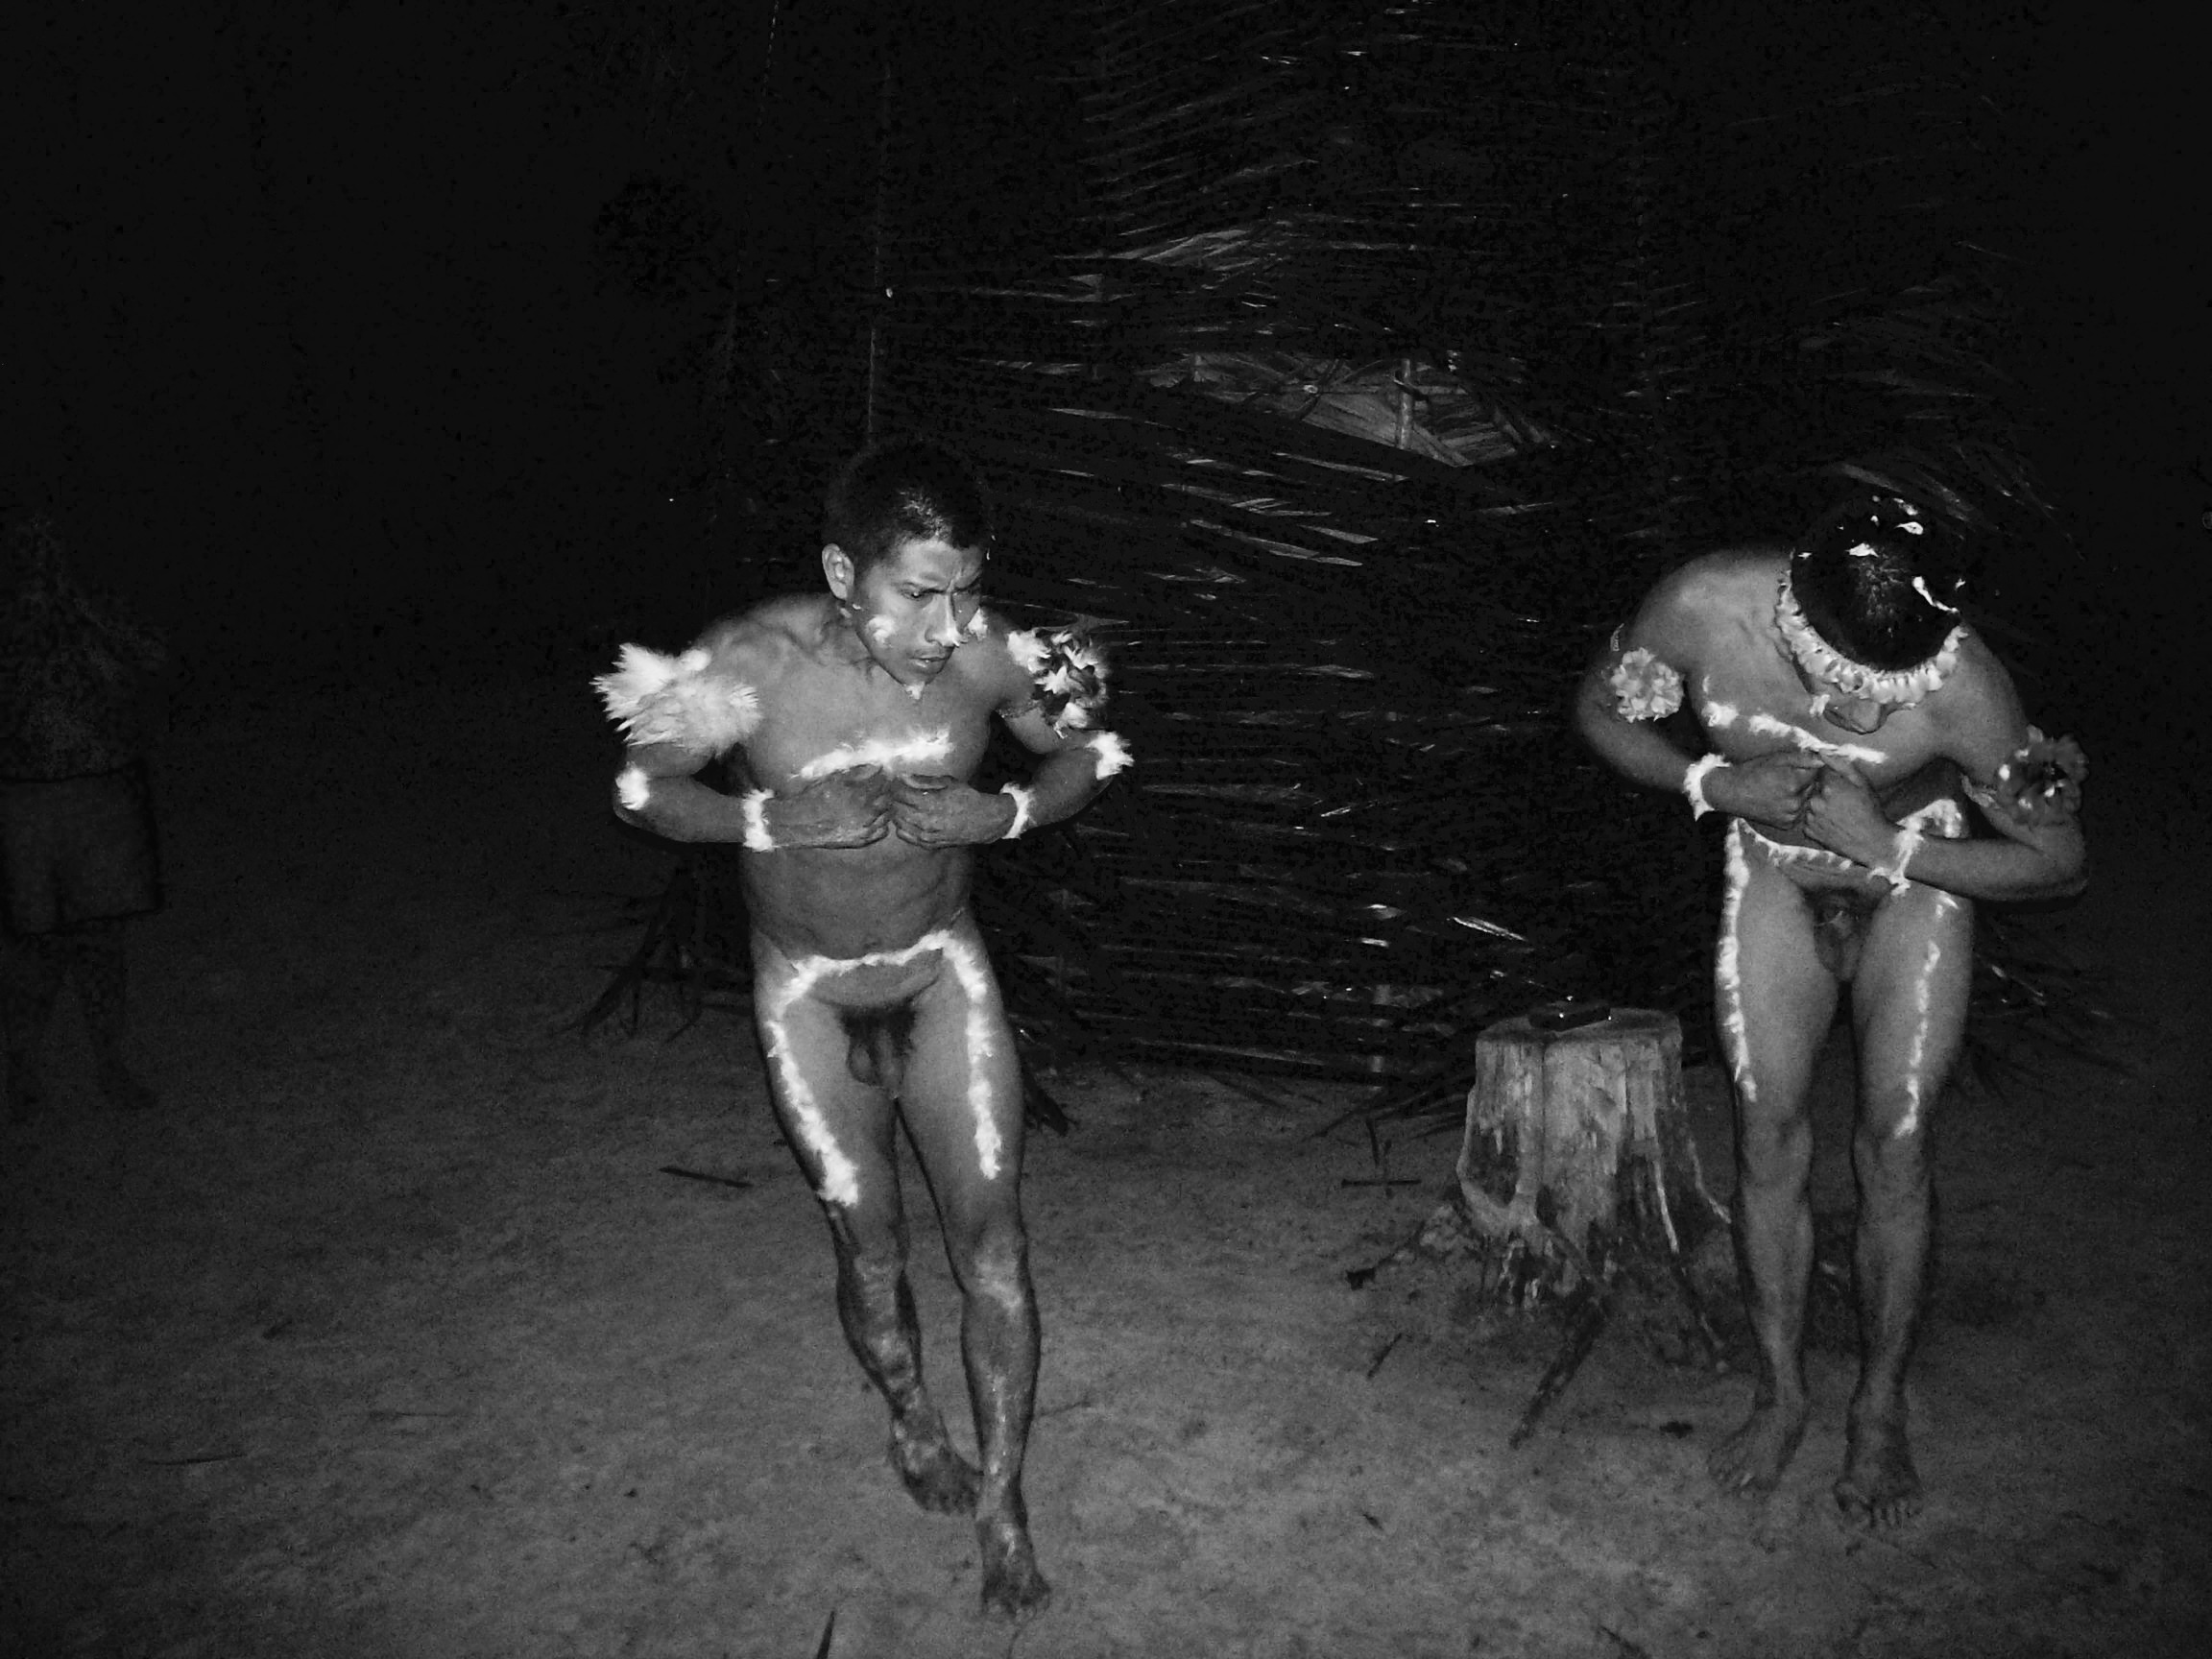
\includegraphics[width=\textwidth]{./imgs/100_1695}
\caption{Os homens trazem os karawara à noite. Ao fundo se vê a takaja. Juriti, 2009.}
\end{figure}

A construção da \emph{takaja} Guajá não obedece a nenhuma prescrição
ritual ou regra de conduta, diferente, por exemplo, da ``\emph{tokasa}''
dos Asurini Akuawá. Andrade observa que para os Asurini ``a colocação das
folhas é feita de tal forma que o construtor termina a tarefa dentro da
\emph{tokasa}. Ele só pode sair de dentro após cantar a \emph{música}
\emph{da} \emph{tokasa} (\ldots{}). Caso a canção não seja logo executada
(pelo construtor ou outra pessoa que a saiba), o construtor pode morrer''
(Andrade, 1992, p. 99--100). Se o evento noturno é de pouco
cerimonialismo e marcado por grande informalidade (como veremos), a
construção da \emph{takaja}, então, se parece com uma atividade
ordinária, quase sem importância. Eu mesmo fui instado diversas vezes
para entrar e conhecer a \emph{takaja} por dentro (sempre durante o dia,
pois à noite tudo é diferente). Ainda que seja construída de uma forma
um tanto deslustrada (sem prédica, cerimônia, ou um mínimo cuidado
ritual), a construção da \emph{takaja} é algo que produz grande alegria
a todos, principalmente às crianças que inserem o abrigo ritual em suas
brincadeiras diurnas, entrando e saindo livremente de lá; ou ainda às
mulheres, que fazem questão de varrer o entorno, antes e depois de ela
ser erguida, e assim passam varrendo durante todo o verão. A
\emph{takaja} na aldeia, nos meses de seca, é algo que os Guajá apreciam
bastante, até guardam certo orgulho por tê"-la ali. Porém é um orgulho
que não parece diretamente relacionado ao cerimonialismo ou qualquer
tipo de sermão, mas a algo de outra natureza --- que eu não saberia
precisar ---, como que relacionado à boa vida do verão e ao prazer que os
homens cultivam em ir ao \emph{iwa} e cantar com os \emph{karawara}. Na
aldeia juriti, a takaja fica exatamente no centro da aldeia, mas nem
sempre foi assim. Os Guajá se lembram que, quando viviam na mata,
construíam a tajaka sempre em um canto da aldeia, a caminho da floresta.
Assim ela é feita na aldeia \emph{Awa} (\versal{TI} Caru) na última sessão
residencial, já a caminho de uma capoeira. A \emph{takaja} não funciona
como uma ``casa cerimonial'' em um pátio central, que congregaria homens
e deuses; ela é um elemento bem mais discreto e minimalista, assim como
é todo o investimento ritual dos humanos (\emph{awa}).

Descrever a \emph{takaja} dos Guajá é quase que descrever um não ritual.
Algo como expor apenas ``negatividades'' em uma interminável lista de
``elementos rituais'' que não encontramos lá. Na composição desse ritual
--- que também podemos chamar de ``cantoria'' (\emph{janaha}), como fazem
os próprios Guajá ---, o ambiente da aldeia em nada se modifica durante as
noites em que ele ocorre: nada é levado ao pátio; nenhuma reza é
realizada; comidas não são preparadas cerimonialmente; e nem mesmo a
caça de animais específicos está prescrita, isto é, não há caças
rituais. Além disso, não há flautas, cigarros, mingaus, bebidas
fermentadas, danças com animais; nem distinção entre ``alimentos
cotidianos'' e ``alimentos rituais'' (como encontramos em diversos povos,
entre eles os Parakanã {[}Fausto, 2001, p. 422{]}), até porque não
existem alimentos no ritual. Observo que, se antes a ideia de \emph{awa
janaha} (``cantoria humana'') expressava o momento ritual da
\emph{takaja}, mais recentemente, sobretudo, os Guajá da \versal{TI} Caru --- onde
há um trabalho de parceria com o \versal{CIMI} --- têm também se referido a ela por
meio de ideias como ``ritual'' e ``cultura''; ou ao menos a estão,
assim, explicando para os interlocutores não indígenas, como a Frente de
Proteção da Funai. É interessante, pois a primeira tradução em português
que encontrei para a ideia de ``cantar na \emph{takaja}'', ainda na
aldeia Juriti, foi a de ``brincadeira'' ou simplesmente ``brincar''
(\emph{pirika}, na pronúncia Guajá). Todos os homens, inclusive os
velhos, vinham falar comigo sobre ``\emph{pirika}'' (que eu no início
entendia como ``brigar'') nos dias que cantariam na \emph{takaja}. Essa
tradução fora"-lhes fornecida pelas pessoas das Frentes de Atração e
funcionários do posto que se referiam ao ``\emph{karawara}'' (tal a
forma que os brancos denominam a \emph{takaja} guajá) pelo mesmo termo
que outras festas maranhenses, como o bumba"-meu"-boi, todas elas --- no
Maranhão e em boa parte do Brasil --- chamadas popularmente de
``brincadeira'' (``brincar o boi'', como se fala no Maranhão). Mais
recentemente, ao menos nas aldeias Awa e Tiracambu (na \versal{TI} Caru), a ideia
de ``brincadeira'' está cedendo lugar a ``ritual'' e ``cultura''.

À exceção da \emph{takaja}, a única preparação especial está no fato ---
desde alguns dias antes de sua montagem --- de que algumas pessoas se
mobilizam para capinar e limpar todo o mato acumulado durante o inverno
no centro da aldeia. A Terra é um local sujo (\emph{manahỹ}) para os
\emph{karawara}, eles não pisariam em Terra se o local não estivesse bem
limpo. Uma vez o pátio limpo, pode"-se começar a montagem da
\emph{takaja}, que é erguida em pouco tempo: cerca de 40 minutos. No
início da noite, os homens começam a entoar seus cantos de maneira muito
potente. E, aos poucos, começam a se adornar. Suas esposas os ajudam a
se paramentar. Quando um homem é solteiro (ou sua esposa ainda é
criança), recebe o auxílio de sua irmã, cunhada, ou até mesmo de outro
homem. A ornamentação consiste em braceletes com penas de tucano,
chamados \emph{jamakwa}, e um cocar formado com as mesmas penas, chamado
\emph{jakỹ ita}. No corpo --- coxas, virilha, torço, braços, rosto e em
volta dos pulsos, como um bracelete --- e nos cabelos são afixadas
penugens brancas da harpia, gaviões ou urubu"-rei. Estas são presas com
resina cheirosa de dois tipos de amescla (breu"-branco), chamadas
\emph{jawarako} (\emph{Trattinnickia burseraefolia}) e \emph{uhuka} (que
não identifiquei). Tais resinas, além de fixar as penas, exalam um odor
muito agradável, mentolado, que é o próprio cheiro dos \emph{karawara}.
Os braceletes de penugem branca podem ser feitos de duas formas: as
penugens são coladas diretamente no pulso com a resina; ou são amarradas
na fibra de tucum, como uma pulseira atada ao punho. Uma vez
paramentados, podem ir para o céu.

A noite já se instalou, e a partir de agora quanto menos luz perto da
\emph{takaja}, melhor. Enquanto se adornam, os homens cantam, e uma vez
prontos se dirigem ao abrigo cantando e dançando com passos específicos:
as duas mãos entrelaçadas sobre o peito e, sem mudar a postura das mãos,
levantam e abaixam o corpo como os movimentos de uma ave a ciscar o
chão. Esta é uma das danças (\emph{panỹ} ``dançar'') executadas pelos
\emph{karawara} no céu e imitadas pelos humanos na Terra. A única
luminosidade em volta da \emph{takaja} vem de uma casa em que um fogo
queima bem baixinho para espantar o frio. A escuridão é uma das marcas
desse momento ritual. Os \emph{karawara} só descem à Terra na escuridão,
pois, mesmo vindo caçar durante o dia, não gostam da luminosidade
terrena. É importante lembrar que toda cantoria na \emph{takaja} é
noturna, e podiamos pensar que, assim como para os \emph{xapiri} do
mundo Yanomami, nossa noite é o dia para os \emph{karawara} (Kopenawa e
Albert 2013, p.55). Os humanos, por isso também, nunca cantam ou dançam
cerimonialmente durante o dia; tampouco existem festas que durem dias
seguidos. Se a \emph{takaja} for feita durante noites seguidas (o que
varia muito), tudo é interrompido na madrugada. Nesse caso, no dia
seguinte todos voltam a suas atividades cotidianas, e à noite uma nova
sessão é iniciada.

A cantoria e a dança se iniciam enquanto, um de cada vez, os homens
adentram para cantar na \emph{takaja}. No início, o clima é de grande
informalidade. Enquanto algumas pessoas estão completamente envolvidas
na cantoria, outras vêm e vão ainda procurando uma refeição para fazer.
Pessoas que não estejam diretamente envolvidas conversam bem alto como
se nada de mais especial estivesse ocorrendo. As crianças correm em
volta da \emph{takaja}, fazendo algazarra, enquanto os adultos estão
compenetrados em cantar. No entanto, nenhum desses acontecimentos afeta
a dinâmica do evento. Lembro aqui que, no falar dos \emph{karawara},
cantar é -\emph{myry} e não ``\emph{jã}'' como na língua Guajá. E na
\emph{takaja}, ao menos nas canções, é observada a língua celeste, que
pode ser traduzida também como uma ``linguagem ritual''. Nesse caso, no
falar dos \emph{karawara}, fala"-se \emph{imyry ta iwapepe jaha} (``eu
vou cantar no céu'')\footnote{Sobre os \emph{karawara} falarem outro
  idioma, Calheiros também observa algo semelhante nos
  ``\emph{karuwara}'' Aikewara: ``(\ldots{}) eles (os \emph{karuwara}) não
  são ``aqueles que se foram'', eles não são seus mortos, seus
  ancestrais, eles são outros, são seus inimigos, falam, inclusive, uma
  outra língua, incompreensível aos ouvidos de um Aikewara médio, uma
  língua que somente os \emph{se'engara'e} (xamãs) dominam (Calheiros
  2014, p. 266).}.

Uma vez dentro, o homem inicia uma sucessão de cantos que são entoados
com toda força, quase sempre se iniciando com o \emph{Makaro janaha},
``canto do (\emph{karawara}) \emph{Makaró}'', que, como já mencionei, é
quase que uma epítome de um grande caçador de porcos e do que sejam os
próprios humanos hoje em dia. Do lado de fora da \emph{takaja}, homens,
mulheres e, por vezes, nos momentos iniciais da noite, crianças, seguem
cantando. É possível perceber o som da voz masculina no interior da
\emph{takaja} se deslocando de um lado para outro, já que o homem que se
encontra dentro está dançando em movimentos circulares. De repente
ouve"-se o barulho de um salto e um silêncio mortal no interior do
abrigo: o homem foi para o céu; ``\emph{oho iwa}'', alguém comenta.
Nessa hora, a esposa, irmã ou qualquer outra mulher ligada ao viajante
celeste inicia um canto frenético. É só a partir daí que podemos
enxergar a importância das mulheres durante a cantoria, pois sem elas
dificilmente os homens conseguiriam voltar para casa (\emph{iwy},
``voltar''). Após subir ao céu, um homem pode permanecer lá por um tempo
relativamente longo que, até onde presenciei, pode variar de 15 minutos
até algumas horas, embora a média talvez seja de meia hora, enquanto o
momento ritual em si pode durar desde duas até seis horas, ou mais.

Wirahoa me explicava que se as esposas não cantassem aqui na Terra, o
marido que estivesse no céu não conseguiria encontrar o caminho de volta
para casa, pois, devido à vastidão do lugar e aos diversos céus que ele
visita em sua viagem, seria muito fácil se perder por lá. O canto das
esposas é o único elo que permite a conexão do céu e da Terra. Enquanto
seus maridos estão na viagem celeste, as mulheres cantam daqui e são
ouvidas por seu duplo celeste (\emph{nima}). Os solidários duplos
celestes das esposas falam ao homem: ``volte para a Terra (\emph{ajwy}
\emph{wype}), volte para ouvir sua esposa cantar, ela está te chamando!''
Por isso, todo canto feminino durante as noites de \emph{takaja} é uma
espécie de chamamento para que o homem volte para casa. Para que não
morra no céu.

Em uma madrugada, já muito tarde, Muturuhũa havia restado sozinho na
\emph{takaja}. Todos já haviam cantado bastante e --- depois de muitas
idas e vindas ao céu --- foram dormir. Muturuhũa foi o último a entrar na
\emph{takaja} e, aparentemente, não havia ninguém para cantar para ele,
pois sua esposa Amỹ Pirawãja estava deitada na rede. Assim que o homem
entrou na \emph{takaja}, a mulher sequer abriu os olhos ou mudou de
posição, mas mesmo deitada em sua rede iniciou um canto baixo e
constante, o suficiente para que seu marido fizesse uma boa viagem. É
claro que outras e outros podem cantar (irmãs ou irmãos, cunhadas ou
filhas); nada o impede. Porém, é muito comum que a esposa cante para o
marido. Ela, portanto, é fundamental em todo o processo de ``ida para o
céu'' (\emph{oho} \emph{iwape}). Sem ela não há viagens celestes nem o
momento ritual na \emph{takaja}. A conjugalidade pontua todo esse
processo, pois são as esposas celestes que cantam, ``lá em cima''
(\emph{wate}), o canto das esposas terrenas. São elas que ouvem as
mulheres da Terra (que para elas são \emph{hapihiara}, seus ``duplos'') e
informam o caminho de volta aos Guajá que estão no céu e, sobretudo, que
é hora de voltar. Minha hipótese é que não podem existir viagens ao céu
(e portanto xamanismo) sem que os homens estabeleçam algum tipo de
relação conjugal com mulheres \emph{karawara}. Essas esposas celestes,
muitas vezes, descem à \emph{takaja} a fim de procurar por seus maridos
terrenos, como aconteceu certa vez em que Wirahoa estava ausente da
aldeia (talvez estivesse no caminho de volta de uma caçada). Sua esposa
Ajruhua foi chamada por outras pessoas para perto da \emph{takaja}, pois
a esposa celeste, \emph{iwa} \emph{nimirikaa} (assim me foi dito ``a
esposa'' e não ``uma esposa'') estava querendo ouvir"-lhe cantar. Mas, como
todos os \emph{karawara}, ela voltou rapidamente para o céu. Quando
conversei depois com Ajruhua sobre a situação, ela respondeu muito
tranquilamente: ``é a mulher do céu, ela veio procurar o marido dela, mas
ele tá caçando!'' O ``marido'' em questão era seu próprio marido.

Enquanto seus pares cantam em volta da \emph{takaja}, um homem, ao
adentrá"-la, permanece no interior ainda por alguns minutos, cantando e
dançando até que consegue subir. Assim como acontece nos sonhos
(\emph{imuhy}), o \emph{ipirera} (couro), o corpo da pessoa, permanece
no interior da \emph{takaja}, despossuído de seu \emph{hajtekera}
(princípio vital). É, portanto, o \emph{hajtekera} que se desprende do
\emph{ipirera}, do corpo, e viaja até o céu (\emph{iwa}). Chegando ao
\emph{iwa}, depois de muito subir, o homem encontra o primeiro patamar
onde só há daquela água quente, '\emph{ya} \emph{haku}, e que, à época
das chuvas, inunda a Terra na forma de grandes temporais. Durante o
verão, quando ocorrem os cantos da \emph{takaja}, o nível de água nesse
primeiro patamar é muito baixo, a lama toma o lugar das águas e o grande
lago de águas borbulhantes e vermelhas lá existente está praticamente
vazio --- esse patamar, também chamado \emph{iwa}, não tem nenhum nome em
especial. A única condição para se fazer a \emph{takaja} é que o período
das chuvas já tenha terminado.

Para chegar à aldeia dos mortos e dos \emph{karawara} é necessário
atravessar este céu intermediário. Uma vez neste primeiro patamar, o
viajante celeste não deve permanecer muito tempo, pois além das águas
borbulhantes (que já mataram muitas crianças \emph{karawara} que sem
querer caíram nesse lago) lá vivem jacarés (\emph{jakarea}) grandes e
famintos (que, segundo algumas versões, comeriam os humanos que lá
chegam). Por isso, deve"-se subir novamente e, agora sim, alcançar a
morada dos \emph{karawara}, também chamada \emph{karawa} \emph{ripa},
``aldeia dos \emph{karawara}'', local onde estão os \emph{harapihiara}
(parentes próximos, cognatos) e \emph{harapihianã} (parentes distantes,
não cognatos), pois os Guajá defendem fervorosamente uma semelhança
direta entre eles e os \emph{karawara}. A partir daí, os cosmonautas
podem acessar outros muitos patamares celestes, que são incontáveis.
Além disso, como escrevi no capítulo 1, o ``céu intermediário'' das águas
quentes não é justaposto aos outros \emph{iwa,} mas se encontra
deslocadamente abaixo. A terra dos \emph{karawara} estaria mais para
cima e para frente, bem distante da \emph{wy} (Terra). O céu que podemos
observar, estando na Terra, é somente este céu intermediário, a primeira
parada dos homens quando estão em trânsito.

Subir é perigoso, sempre. É uma atividade ultra especializada. Os
\emph{karawara} convidam insistentemente os homens para que subam ainda
mais, a outros céus, para que comam banquetes magníficos em outras
aldeias; para que adquiram outras esposas celestes; conheçam outros
seres; ouçam outros cantos e vejam outras danças. Os humanos, no
entanto, sabem que isso implicaria sua morte, já que, devido à
distância, não ouviriam mais suas esposas cantando e se perderiam para
sempre. Não se deve andar (\emph{wata}) muito no \emph{iwa}. O canto das
mulheres terrenas é ouvido como um canto de procura, e os homens falam
para os \emph{karawara}: ``estão ouvindo a minha esposa cantar na Terra?,
ouçam, ela está me procurando, por isso está cantando, tenho que
voltar''. Os \emph{parentes} celestes ainda perguntam sobre as mulheres
terrenas, pois nutrem grande interesse por elas. Os humanos devem
explicar que elas ficaram na Terra, pois não podem subir, mas os
\emph{karawara} insistem para que os humanos as levem até lá. Uma vez,
ao serem indagados por mim sobre a possibilidade de as mulheres irem ao
\emph{iwa}, foram taxativos dizendo que elas não podem ir, pois não
saberiam como chegar, além de serem cobiçadas pelos \emph{karawara}
celestes. Em outras palavras: elas morreriam. Estamos vendo então que,
por baixo de um verniz de bem"-aventurança e satisfação, há também morte
e disputa por mulheres, envolvidas na relação entre \emph{awa} (humanos)
e \emph{karawara}, cabendo aos humanos administrar esta tensa e delicada
relação. Quando as pessoas mencionam essa comunicação melódica entre
mulheres na terra e homens no espaço celeste, afirmam que o canto das
mulheres não são apenas um canto de referência para os homens ouvirem
desde o céu, mas se trata de um diálogo como certa Wama'axia (uma mulher
da aldeia Tiracambu) me revelou. Ouvindo uma gravação de aúdio de quando
seu pai Akamatỹa estava no céu e sua esposa, Pinawãxika, cantava na
terra, ela explicou que naquele canto a mulher falava ao homem ``volte
para casa'' ``você já comeu?'', e em paralelo o marido cantava ``eu já
comi guariba'' e ``agora eu cheguei aqui no chão'' (voltei do céu). Essa
comunicação entre esposas que cantam da terra e homens que as escutam do
céu é, além de poética, metafisicamente complexa, pois os homens podem,
só pelo fato de responderem à esposa, voltar à terra imediatamente.
Imagino que, se tirarmos por esse caso específico, a própria palavra de
uma mulher pode produzir a volta do marido. As evidências são sempre
baseadas em fragmentos como esse acima, pois assim também o é o estilo
vocal Guajá, cheio de cortes, repetições e paralelismos (com 2 pessoas
cantando em paralelo em ``diálogo'' ou não).

A visita dos humanos ao \emph{iwa}, durante a \emph{takaja}, é (lá nos
patamares superiores) marcada por canto (\emph{janaha}), dança
(\emph{panyha}) e comensalidade (\emph{i'uha}). É disso que tratam os
encontros celestes, uma vez que caçar (e comer) e cantar é o que marca
boa parte da vida humana. Os diversos \emph{karawara} entoam seus cantos
característicos e o fazem sempre de uma forma mais bela que os
visitantes humanos; e ainda pedem para que os humanos cantem. Os
\emph{karawara} ainda dançam com suas flechas energizadas nas costas,
coreografias repletas de brilho; são as mesmas flechas que utilizam para
caçar na Terra e que matam suas presas sem lhes causar ferimento. Os
raios do céu, principalmente aqueles que aparecem à noite, são o
resultado das flechas com energia (\emph{tata}) desses \emph{karawara},
e quando alguém olhar para o céu e notar os raios, certamente exclamará:
``\emph{karawara} \emph{panỹ!''}, os ``\emph{karawara} estão dançando!'' Por
isso, na Terra, outra forma de os homens dançarem fora da \emph{takaja}
é colocarem cera de maçaranduba ou jatobá na ponta de uma taquara (ou
outra madeira fina), acender e dançar com ela apoiada sobre os ombros,
tal como os \emph{karawara} com suas flechas, o que causa um efeito
visual fantástico. Há ainda dois \emph{karawara} chamados \emph{Japu}
\emph{Jara} (pássaro japu) e \emph{Japini'i Jara} (xexéu) que, por serem
construtores de tapiris no céu, lá dançam com palhas sobre as costas.
Por isso os homens, ao cantar seus temas na \emph{takaja}, dançam
segurando palhas secas nas costas, como esses \emph{karawara}.

Quanto à comensalidade, ela parece ser uma espécie de ``oferenda às
avessas'', diferente de outros povos Tupi que preparam rituais com
banquetes específicos para suas entidades sobrenaturais que aqui descem
para se alimentar (como já expus anteriormente). Entre os Guajá, são os
\emph{karawara} que lhes oferecem comida. Como já sugeri, há grande
fartura no \emph{iwa}, já que os caçadores magníficos que lá habitam
conseguem carnes com tanta facilidade que nem sequer as estocam. Além
disso, a farinha é branca e quase doce (\emph{hee'ẽ}) de tão gostosa, os
frutos são maiores e as quantidades de mel, descomunais. Desta forma os
\emph{karawara} disponibilizam toda essa fartura para os humanos que lá
conseguem chegar, quase que um oposto do que vemos em outras formas de
xamanismo, em que são os deuses que descem para comer. Os homens que
alcançam o céu são unânimes ao lembrar que os \emph{karawara} tentam
prendê"-los lá pela fartura e abundância das refeições.

Assim, uma vez no \emph{iwa}, um homem encontra seus parentes, canta e
come com eles, escutando seus conselhos, desde a escolha de um nome,
notícias sobre caçadas, sobre a cura de enfermos (quando existem), e até
mesmo bens são disponibilizadas pelos \emph{karawara}. Wirahoa confirmou
já ter trazido alguns cartuchos (de espingarda calibre 20) que ganhou de
presente dos \emph{karaia} celestes. Pessoalmente, tive o prazer de
presenciar a preparação dos caçadores para uma caçada de porcos, cujo
rastro da vara aparecera no dia seguinte a uma noite de cantoria na
\emph{takaja}. Wiraho me disse com tranquilidade que havia pedido para
seus \emph{parentes} mandarem os animais para que fossem caçados. Nunca
encontram \emph{Maira} no \emph{iwa} durante a época em que sobem, pois
o verão (\emph{kwarahy mehẽ}) é a época em que \emph{Maira} (além de
alguns \emph{karawara} que não saberia apontar) se ausenta para longe e
vai para a ``casa de seus sogros''. Durante as noites de \emph{takaja},
os Guajá só se encontram com os parentes mortos (tornados
\emph{karawara}, como veremos logo adiante), além dos \emph{tenetehara},
dos \emph{karaia} celestes e dos diversos \emph{jaras} que já elenquei.

\section{\emph{Aru karawara}, trazer os \emph{karawara}}\label{aru-karawara-trazer-os-karawara}

Uma das coisas mais impressionantes no momento ritual da \emph{takaja},
tanto quanto a subida dos homens ao céu, é a descida dos \emph{karawara}
para ali cantar e dançar. Uma vez que um homem vai para o céu, o
silêncio reina no interior da \emph{takaja}; só é ouvido o som da
cantoria externa, sobretudo das mulheres. Esse estado permanece por
longos minutos (10, 15 ou mais). Todavia, passado algum tempo as folhas
da \emph{takaja} tremulam de cima abaixo e ouve"-se o barulho de um pulo:
dois pés pisaram o chão simultaneamente, o que indica que algum
visitante celeste veio à Terra (\emph{wya}) cantar. Quando sobem, seu
\emph{ipirera} (corpo) fica no interior da \emph{takaja}, vazio,
utilizado como uma pele pelos \emph{karawara} (sejam, onça, gavião,
pássaros, marimbondos, \emph{karaia}, \emph{tenetehara} e a infinidade
de seres que vive no \emph{iwa} e desce para cantar). Para quem sobe ao
céu é dito que ``traz os \emph{karawara}'', \emph{ru} \emph{karawara}; uma
vez no \emph{iwa}, ele diz aos seres de lá: ``Desçam, vão ver seus
parentes na Terra!'' Alguns são bem"-vindos, outros (como as onças
celestes) devem ser espantados. Para isso, uma criança, se alguma ainda
estiver acordada, uma mulher ou um homem bate com vigor nas paredes de
folha da \emph{takaja}. Um pedaço de pau (\emph{wira}) é utilizado para
bater, visando a enviar o visitante indesejado de volta para o céu. A
\emph{takaja} é um local perigoso, pois é aberta a diversos tipos de
seres, inclusive a alguns que intentam levar esposas da Terra, ou mesmo
sair da \emph{takaja}. Por isso, os homens que os trazem devem se
entender bem com eles e, em alguns casos, as pessoas os devem espantar
de volta, batendo nas paredes. Durante a cantoria, não é permitida a
entrada de nenhuma mulher ou criança no abrigo.

A \emph{takaja} Guajá, tal como ocorre com outros povos, como os
Parakanã (Fausto 2001, p.281) e Asurini do Xingu (Müller 1990,
p.151--154), seria algo como um ``aprisionador ou receptáculo de
espíritos'' (Fausto 2001, p.281), tal uma transformação do maracá, como
pontua o autor:

\begin{quote}
\emph{A ideia de que os espíritos se manifestavam através dos maracás porque
estavam dentro dele é expressa por autores que consolidaram o material
quinhentista: `o maracá, instrumento sagrado dos tupinambás, possuía uma
função definida nos rituais, parecendo fora de dúvida que estava nele o
espírito envocado (Fernandes 1970: 75--76); `o maracá servia de
receptáculo ao espírito' (Metraux 1979: 60). O maracá seria, pois, uma
tokaja, que atrai e contém os espíritos, os quais só os pajés eram
capazes de ouvir (Fausto 2001, p.281)}.
\end{quote}

A \emph{takaja} aqui, tal a analogia de Fausto a partir do material
quinhentista, pode ser pensada como esse grande objeto atrator e
aprisionador e parece operar como um grande instrumento musical, uma
grande caixa de ressonância para os \emph{karawara} que descem à Terra
para cantar.

Cada \emph{karawara} detém especificidades em seus cantos, de modo que
todas as pessoas que estão do lado de fora da \emph{takaja} sabem
exatamente qual ser está em seu interior. E todos descem à
\emph{takaja}: onça (\emph{jawara}), papa"-mel (\emph{haira}), jiboia
(\emph{majhua}), jacaré (\emph{jakarea}), gavião (\emph{wirahoa}),
pererecas, poraquê (\emph{marakya}), dentre outros. Além desses, os
\emph{karaia} e \emph{kamara} celestes também descem. Os \emph{karawara}
que descem do céu, além de cantar, emitem os sons característicos de
seus duplos terrestres, sugerindo que, sim, os \emph{karawara} são
versões humanas e celestes (isto é, duplos) de animais terrenos. Os
Guajá dizem que quem emite os rugidos e cantos de animais são os filhos
dos \emph{karawara} que os acompanham à \emph{takaja}, pois esses, por
serem crianças, ainda não sabem cantar. Desta forma, é possível ouvir a
onça e seu rosnado; o som gutural de porcos; o canto do gavião; e até
mesmo um improvável morcego (\emph{arira}) que aqui veio cantar. Alguns
seres animais, como os \emph{Jakara} \emph{Jara} (que vivem no patamar
alagado) e \emph{Wri} \emph{Jara} (um capelão agressivo de cor
vermelha), também vêm para a \emph{takaja}.

À medida que os homens saem da \emph{takaja} para cantar do lado de
fora, quem está ali são os próprios \emph{karawara}, que param em frente
as mulheres e crianças, cantam"-lhes, sopram"-lhes e por meio das canções
contam suas epopeias, falam sobre a saudade de uma Terra e um tempo
distante ou cantam as maravilhas que há no céu. Nas noites de
\emph{takaja}, as aldeias ficam repletas de \emph{karawara}. Esses
\emph{karawara} se relacionam diretamente com aquele homem específico,
como parceiros ou mesmo ``espíritos auxiliares''. Cada homem se
relaciona com um conjunto de espíritos específicos no céu, e são eles,
da confiança dos humanos, que descem à Terra. Após algum tempo no
\emph{iwa}, é o momento de o homem retornar. A descida, como me foi
relatada por Hajmakoma'ã, é suave e pode ser comparada à queda de uma
``folha''. Esta seria mais uma razão para os meninos jovens não irem ao
\emph{iwa}: eles não saberiam como descer, poderiam cair na descida e
morrer. É muito comum, nas primeiras tentativas de ida para o céu,
jovens de 15 anos tentarem subir e, mesmo paramentados, se frustarem em
tentativas de alcançar o céu. São necessárias muitas sessões iniciais
até que os jovens aprendam. Houve noites em que os homens tiveram que
ser breves, com uma duração ritual muito curta (cerca de duas horas),
pois o \emph{iwa} naqueles dias estava insuportavelmente quente, e os
humanos não aguentaram permanecer por lá. Em todo caso, é esse \emph{iwa
rakuha}, ``calor do céu'', que os \emph{karawara} trazem na descida à
Terra, sopram nas esposas e crianças do seu parceiro e que tem funções
terapêuticas.

O processo de cura consiste basicamente em trazer o ``calor do céu''
(\emph{iwa} \emph{rakuha}), esse ar terapêutico que é soprado pelo
homem"-xamã em diversas partes do corpo da pessoa. Esse calor, tanto atua
de forma preventiva, fortalecendo o corpo, como pode curar um enfermo,
se administrado em doses mais intensas. O que os \emph{karawara} fazem
na Terra é (1º) ``cantar'' (\emph{jã}) e (2º) ``soprar'' (\emph{pyy});
hoje em dia, muitas pessoas da \versal{TI} Caru têm chamado isso de ``rezar'', em
português. A ideia do sopro é que as pessoas fiquem bem, sem doença:
\emph{a'e kĩja}: ``ficar assim todo tempo'', sem doença. Essa é uma das
funções do sopro, ``\emph{iku katy}'', ``ficar bem''. Os \emph{karawara}
entram no corpo do seu parceiro (``irmão''), \emph{hapija perera},
``pele do irmão'', como que se vestindo com sua pele (\emph{ipirera})
para atuar na Terra. Outra forma de mencionar essas curas é \emph{ru
iwa} \emph{janaha}, ``trazer a música do céu''. Os \emph{karawara} e a
cura estão diretamente relacionados. É pelo canto que os homens se
comunicam com os \emph{karawara} que lhes auxiliam nas curas. O canto é
quase um bem material, algo externo produzido pelos \emph{karawara} e
utilizado pelos humanos.

Quando os \emph{karawara} descem do céu vestindo a pele dos humanos e
saem da \emph{takaja} em direção a suas esposas e filhos para soprá"-los
(\emph{pyy}), sempre haverá uma mistura entre \emph{karawara} e humano ---
é como se o homem o trouxesse junto com ele. E só quem vê os
\emph{karawara} são os homens que cantam e curam. Em outra
interpretação, os \emph{karawara} ficariam dentro da \emph{takaja}, e
quem sai seria o próprio homem para soprar. Segundo me informou Wirahoa,
os \emph{karawara} ``falam'' com os Guajá de dentro da \emph{takaja}.
Ideias como \emph{xá} \emph{iwa} (``olhar o céu'') \emph{takaja janaha}
(``o cantar da \emph{takaja}''), \emph{ru karawara} (``trazer
\emph{karawara}'') e \emph{ru hakuha} (``trazer o calor'') são todas
sinônimos para ``curar''. Enquanto os \emph{karawara} estão em Terra eles
sopram os vivos e tiram as doenças. Trata"-se de um ``xamanismo padrão'',
acessível a todos os homens (quase como uma imposição de gênero), e está
longe de ser um conhecimento especializado. Se perguntarmos a qualquer
um, na aldeia Juriti, quem lá saberia ``tirar'' ou ``soprar'' doenças
(\emph{hahy}, ``dores''), todos os homens adultos serão apontados, pois
todos conseguem ir para o céu e trazer o ``calor'', o que não quer dizer
que todos tenham o mesmo nível de excelência. Por isso, Xiparamyxa'a, um
homem mais velho, é considerado o melhor curador da aldeia. Muitos
homens recorrem a ele quando eles mesmos não conseguem curar seus
parentes próximos. Lembro ainda que não encontrei um termo na língua
Guajá para o especialista em cura.

As doenças, como já vimos, têm causas variadas, e a terapêutica Guajá
mistura os cantos e os remédios tradicionais. Houve uma ocasião,
enquanto trabalhávamos na roça, em que encontramos um pequeno veado
foboca (\emph{arapaha'ia}), que logo fugiu. Na mesma tarde, o jovem
Juxa'a, que estava conosco na roça, caiu doente com muita febre e
calafrios. Sabemos que os veados são animais de criação dos \emph{ajỹ},
por isso lançou"-lhe \emph{ha'aera} (raiva). Naquela mesma noite, seu
padrasto teve que tirar"-lhe a doença (\emph{hahy}). Tratava"-se de um mês
de inverno, e nas chuvas os homens não sobem ao céu pela \emph{takaja},
trazem os \emph{karawara} para dentro de seus corpos com o canto, o
único agente concreto do xamanismo Guajá.

Os Guajá não utilizam tabaco nem as bebidas fortificantes que seriam
consumidas pelo curador. O máximo que utilizam são os remédios da
floresta como auxílio da cura, porém o básico é o canto (\emph{jã}) e o
sopro (\emph{pyy}): o canto, para trazer o \emph{karawara}, e o sopro,
para tirar a doença. Além da \emph{takaja}, há pelo menos uma forma de
trazer os \emph{karawara} à Terra. São esses cantos noturnos, em casa,
na rede, quando o homem abandona seu corpo e traz o \emph{karawara} para
curar quem quer que seja. Quando um homem canta, o \emph{karawara} se
instala em seu peito que lhe comunica os procedimentos. É isso que
orienta os homens nas curas, tal como espíritos auxiliares. E o homem
canta ainda mais alto. Essas curas são chamadas simplesmente de
\emph{karawara} ou \emph{ru} \emph{karawara}, ``trazer \emph{karawara}'',
tal qual a acepção comum de ``feitiço'' que vimos em outras paisagens. Os
\emph{karawara} Guajá se conectam parcialmente com essa ideia de feitiço
e contra"-feitiço, mas que não podem ser traduzidos literalmente assim,
pois, antes, são seres que dominam a cura, a qual também é chamada
``\emph{karawara}''. O agente terapêutico (chamemos assim) soprado pelos
homens, o calor do \emph{iwa}, serve para tirar o agente patogênico
(\emph{ha'aera}) do corpo das pessoas. Por isso, para os animais, o
\emph{ha'aera} é visto como \emph{karawara}. O ``\emph{ha'aera} é o
\emph{karawara} do capelão'', repetindo o que alguém me disse certa vez.

A cura feita sob orientação dos \emph{karawara} consiste em que o
homem"-xamã molhe com saliva seus dedos indicadores e imprima pequenos
pontos úmidos nos braços, troncos, pernas, ou outra parte que esteja
dolorida ou doente. Após essas marcas serem feitas, deve"-se soprar
bastante, além de cantar com intensidade. O sopro, tanto na
\emph{takaja} quanto durante a época das chuvas, nessas seções privadas,
é feito nos braços e na cabeça. Cada braço é soprado, ao fim de cada
sopro passa"-se a mão, e o processo termina com um sopro forte na cabeça;
repete"-se isso diversas vezes, interrompendo"-se apenas para cantar. Esse
é o procedimento básico para tirar o \emph{ha'aera} de alguém que foi
atacado por esses princípios mortais. A saliva é dita esfriar o corpo
(\emph{ipirera}) da pessoa que estiver com febre. Se o fígado (órgão
destacado como de grande importância vital) estiver ruim, por exemplo,
imprimem pontos de saliva na barriga e costas; o mesmo ocorre com o
coração, dores nas juntas, musculares, cabeça, ou qualquer outra parte
magoada. Eu não saberia explicar a função da saliva nesse processo, mas
ela parece oscilar entre um antitérmico, condutor do sopro e uma espécie
de abridor de poros por onde o sopro entraria. De forma análoga,
descrevendo uma sessão xamânica, Fausto destaca que na cura Parakanã,
aquele que controla e sonha com os xerimbabos oníricos, além da fumaça
do cigarro e do sopro, esfrega sua saliva no corpo do enfermo a fim de
lhe imprimir a devida cura (Fausto, 2001, p. 373).

\begin{center}
***
\end{center}

Para finalizar esse tópico, o rodízio de homens que entram na
\emph{takaja} segue uma ``ordem'' estabelecida de acordo com a situação.
Se participam cinco homens, o primeiro a entrar será o primeiro a
reentrar na \emph{takaja}, depois que todos seus companheiros já o
tiverem feito. À medida que um homem sai da \emph{takaja}, outro entra
imediatamente, ela não permanece vazia nem por um minuto. Depois de
outro período, entra um terceiro, e assim sucessivamente. A ordem
inicial parece aleatória, porém, quando o último homem a entrar sai da
\emph{takaja}, o que iniciou o processo retorna a ela, e a mesma ordem é
obedecida. Na aldeia Awá (\versal{TI} Caru) acontecia também de entrarem dois
homens ao mesmo tempo. Depois de duas ou três entradas na \emph{takaja}
(e algumas boas horas de cantoria), já é alta madrugada, o relógio marca
três horas da manhã, e à medida que os homens saem do abrigo ritual,
voltam para suas casas levando o calor do céu para soprar em seus filhos
e esposas. A ``brincadeira'' (para evocar uma tradução indígena) acaba
gradativamente. O silêncio vai nublando a aldeia. Em seu pátio central,
só restará uma mulher, solitária, cantando para que seu marido retorne
em segurança do \emph{iwa}, para, então, poderem dormir em paz naquela
noite.

\section{Ritornelo}\label{ritornelo}

``Depois que morre, vira \emph{karawara}!'', é o que muitos diziam quando
conversávamos sobre a morte. Ao falarem sobre a morte, empregam como
sinônimo o verbo ``subir'' (em português mesmo). Além disso, na língua
Guajá morrer (\emph{manũ}) é referido como \emph{oho iwape} (``ir para o
céu''), a mesma ideia utilizada para descrever o momento ritual da
\emph{takaja}; ou ainda \emph{ikwẽ iwape} (``permanecer no céu''). Além
dessas, outra forma pela qual se referem à morte (\emph{manũ}) é
\emph{karawara} \emph{pyhy}, literalmente, ``os \emph{karawara} pegaram''.
Os Guajá não gostam de conversar sobre a morte e sobre os detalhes da
nova vida que um dia todos experimentarão no \emph{iwa}. ``Eu não sei
não, Uirá!'', era o que me respondiam quando eu perguntava mais sobre os
\emph{karawara} (a quantidade de animais que esses seres caçavam; como
carregavam os animais para o céu; como tiravam embira para amarrá"-los;
como ajudavam nas curas; etc.); ou mesmo quando se tratava de discorrer
sobre a morte em geral.

Existe um \emph{karawara} chamado \emph{Kirimixixa'a} que é o
responsável por ressuscitar o morto quando este chega no \emph{iwa}
(cujo duplo terreno é um tipo de marimbondo que vive na beira de rios e
igarapés e, segundo os Guajá, ``gosta de cavucar a terra''). Lembremos
que, após a morte, é o \emph{hajtekera}, o ``princípio vital'', que vai
para o \emph{iwa}. Portanto, é essa parte da pessoa que renasce no
\emph{iwa}, em forma de \emph{karawara}. Quando um morto chega ao
\emph{iwa}, \emph{Kirimixixa'a}, que é uma espécie de xamã celeste,
habitante de um patamar distante, é avisado por seu filho. Então, ele
desce até os patamares inferiores, que é onde chegam os mortos. As
feridas do morto são limpas com aquela mesma água vermelha e quente
('\emph{y rakua}) que só existe no \emph{iwa} e que os humanos não podem
pisar, nem os \emph{karawara} podem beber. Trata"-se de uma água curativa
capaz de cicatrizar qualquer ferida e esquentar um \emph{hajtekera} que
jaz frio.

Deitado, desfalecido, em uma rede de fibras brancas, a pessoa é soprada
(\emph{pyy}) por \emph{Kirimixixa'a}. Este é o sopro que auxilia na cura
das feridas e no alívio das dores. Além do sopro e da água
ressuscitadora, esse \emph{karawara} lança"-lhe \emph{tata}
\emph{hatỹma'a} (``fogo"-energia saudável"-forte''), a mesma energia
brilhante produzida pelas flechas mágicas dos \emph{karawara} quando
dançam (que são vistas como raios) ou caçam (que matam a caça sem a
ferir), e ainda compõem os cartuchos dos \emph{karawara} que caçam com
espingarda. Uma energia brilhante (como o \emph{flash} de minha máquina
fotográfica) constituinte de vários fenômenos do \emph{iwa}. Após esses
cuidados, \emph{Kirimixixa'a} adorna o recém"-chegado tal como um
\emph{karawara}: se for um homem, com as respectivas penas e cocares;
caso seja uma mulher, com a saia de penas de tucano confeccionada por
sua esposa. Após adornado e curado, \emph{Kirimixixa'a} envolve o morto
na rede (\emph{ikaha}) em que está deitado --- tal como um casulo. Após
abrir a rede, o morto está ressuscitado como um \emph{karawara}.

Quando acordar no \emph{iwa}, o recém"-chegado tem vontade de voltar à
Terra para rever sua esposa e os filhos. Mas os \emph{karawara} não
deixam que isso ocorra. Em pouco tempo, o morto passa a guardar poucas
lembranças (\emph{imarakwaha}) de sua vida terrena, até esquecer
completamente que um dia foi humano. A vida como \emph{karawara}
facilmente suplanta a vida como \emph{awa}. Após a morte de
Pinawataxa'a, em 2009, seu irmão, Wirahoa, me disse que o encontrou no
\emph{iwa} na ocasião de uma \emph{takaja}, passados poucos meses após
sua morte. Nessa ocasião, Pinawataxa'a, o recém"-morto, se recordava
muito pouco de seu irmão que ia lhe visitar no céu. Wirahoa me explicou
que, por haver muita comida, mulheres e belezas no \emph{iwa}, é fácil
esquecerem a vida na Terra (\emph{wya}). É por esse mesmo motivo que os
humanos devem esquecer completamente o morto, tal como um processo de
duplo esquecimento: em que os mortos --- estando lá --- esquecem os vivos; e
os vivos --- estando aqui --- esquecem os mortos. Quanto à ``vida eterna''
(\emph{ikwẽ iwape}, ``permanecer no céu''), ouvi tanto que os
\emph{karawara} nunca envelhecem quanto que têm o dom do
rejuvenescimento eterno e são tornados jovens a cada vez que envelhecem,
pelo mesmo processo energético de \emph{Kirimixixa'a}.

Se morrer é subir, como me relataram inúmeras vezes, o momento ritual na
\emph{takaja}, também dito subir, ou \emph{oho iwape} (``ir para o céu''),
é uma pequena experiência de morte. Os homens que vão para o \emph{iwa}
durante essa cerimônia chegam vestidos como mortos"-\emph{karawara}, com
vestes idênticas às que utilizarão um dia, após lá renascerem como
\emph{karawara}. Os homens, tal como xamãs (embora essa função entre os
vivos não seja explícita), experimentam em vida --- com suas vestes,
canções e viagens ao céu --- as sensações que são vivenciadas plenamente
após a morte. Uma vida cheia de dança, canto e abundância.

Os \emph{karawara} se realizam enquanto ação pois existem como
entidades, e vice"-versa. Pensá"-los, porém, em termos identitários e
afirmarmos algo do tipo ``Os \emph{karawara} são desta ou daquela forma!''
não é o que sugiro aqui. Como vimos, eles são seres do tipo entidades
celestes, destino dos vivos, ao mesmo tempo que agem como agentes
noogênicos, do tipo substâncias extra naturais que realizam curas e
trazem saúde. Assim, os \emph{karawara} também parecem recolocar em
outros termos a relação \emph{riku} que --- se pelo entendimento da
conjugalidade e da propriedade (como no caso das flechas) é traduzida
por ``criar'' --- a relação dos \emph{karawara} com seus \emph{nima}
(``versões'', ``duplos'') terrestres não sugere ``domínio'', nem ``controle'' ou
mesmo ``criação''; mas, sim, ``estar associado a''. A relação \emph{riku},
por isso, pode ser pensada como aquela que relaciona e associa seres,
não somente logicamente, mas consubstancialmente, e que, ora é uma
relação de ``criação'', ora de ``associação'', isto é, de ``estar com''. O
\emph{riku} é um processo de cognação entre diferentes seres do mundo:
maridos e esposas; pais e filhos; mulheres e animais de criação;
caçadores e suas flechas; humanos e duplos celestes; \emph{karawara} e
duplos terrenos; \emph{ajỹ} e animais; nomes e pessoas; animais
\emph{jara} e seus \emph{nima} (como a relação entre um veado e uma
paca); e tantas outras relações que vimos aqui. E essa ``teoria da
relacionalidade generalizada'' (para recolocarmos os termos de Viveiros
de Castro), cujos polos são denominados \emph{jara} e \emph{nima}, nem
sempre implicará controle ou domínio, como comprova o exemplo dos
\emph{karawara}.

A caça, como um ponto importante na vida dos Guajá, articula muitas
relações, como vimos, porém o objetivo deste livro, mais do que tirar
qualquer conclusão generalista, é apresentar os dados de pesquisa e pôr
em relação diferentes aspectos da vida dos Guajá. Um mundo onde haja
caça abundante é fundamental, tanto para os Guajá, quanto para os
\emph{karawara}, caçadores que vêm caçar na Terra. Nas aldeias Guajá,
nos dias de hoje, sem dúvida, o que mais preocupa as pessoas é a
depredação ambiental que acarretará, todos afirmam, o fim da floresta e,
consequentemente, o fim da caça, da comida e, portanto, da vida. Como
parece ter ficado claro durante nosso percurso até aqui, o cenário onde
esse drama se desenrola, é uma das regiões mais desmatadas da Amazônia
(e talvez do planeta). Os Awá estão vivendo um momento crítico de sua
história. A desintrusão da \versal{TI} Awá em 2013/2014 revelou uma terra
devastada; na \versal{TI} Caru temos o mesmo quadro, porém este é agravado pelo
impacto da Estrada de Ferro Carajás (\versal{EFC}) em que duas aldeias estão
quase à margem da ferrovia, separadas apenas pelo rio, e cuja duplicação
será feita em breve. Os Guajá sempre foram muito generosos comigo, e
penso que diversas vezes me pouparam do grande descontentamento e
desilusão que sentem pelo mundo dos \emph{karaia} --- o meu mundo --- que em
menos de duas décadas transformou radical e perversamente sua forma de
vida. Os fatos que mais lhes causam tristeza são a derrubada das
florestas para a abertura de roças e a exploração ilegal de madeira, tal
como ocorre hoje, principalmente na área indígena Awá. Isto, no entanto,
não implica somente a morte da vida da floresta e o fim da vida de
caçador, mas interfere na ecologia dos \emph{karawara} pois, como vimos,
eles também precisam das matas para caçar.

É quase inevitável que hoje em dia um etnógrafo que trabalhe, seja na
Amazônia ou em qualquer outro contexto etnográfico onde existam abusos e
ataques a direitos básicos da vida das pessoas, destruição ambiental e
nenhuma salvaguarda a esses direitos, não seja sensibilizado por esses
problemas e arremate suas reflexões teóricas apontando para um futuro
desanimador às pessoas que tanto lhe ensinaram. É difícil escrever sobre
tais temas, quanto mais quando vimos a força e a vitalidade desse
coletivo humano que, sem dúvida, foram as pessoas mais especiais e
encantadoras que conheci em toda minha vida. Ainda assim, os Guajá, eles
mesmos, me atentaram para algo que vários povos ameríndios nos vêm
alertando há tantas décadas (e até mesmo séculos), isto é, o mal que o
``homem branco'' tem causado à Terra, sem ao menos tentar compreender
quais serão as consequências de suas atitudes. A ``versão Guajá'' para
essa ``queda do céu'' diz respeito à bem"-aventurança dos \emph{karawara}.
Explicando melhor, os \emph{karawara} estão vivos ajudando os humanos,
porque os humanos estão se relacionando com os \emph{karawara}, e mais,
com a floresta; mantendo a caça abundante sem destruir o ambiente. A
possibilidade de vida na Terra é a mesma que propicia a vida no céu,
pois sem a caça, o mel e a água terrena os \emph{karawara} morrem. O
equilíbrio ecológico e cósmico é dado nessa relação; afinal, como vimos,
é um \emph{karawara}, \emph{Japu} \emph{Jara}, que controla as
distâncias entre os diversos \emph{iwa} e a Terra, as mantém em uma boa
distância e controla os níveis do universo. O fim da vida celeste devido
à penúria alimentar é o fim da vida no cosmos. Os Guajá nunca defenderam
diretamente uma teoria fatalista oriunda do desmatamento, mas sugeriram,
em diversos momentos, o descontentamento dos \emph{karawara} para com o
fim da floresta; e isso acarreta apreensão e tristeza aos humanos. Os
\emph{karawara} são os mais interessados em que as florestas fiquem em
pé, pois seu mundo está em uma relação de continuidade com o nosso. Os
próprios \emph{karawara} conhecem bem a Terra (\emph{wya}) pois aqui já
viveram antes da grande separação e, como vimos, nunca deixaram de
``estar junto'' (\emph{riku}) a nós.
